\documentclass[a4paper, 12pt]{book}
%\usepackage[T1]{fontenc}


\usepackage[a4paper, left=2.5cm, right=2.5cm, top=3cm, bottom=3cm]{geometry}
\usepackage{times}
%\usepackage[latin1]{inputenc}
\usepackage[spanish]{babel} %comentar linea si tu memoria es en ingles.
\selectlanguage{spanish}
\usepackage[utf8]{inputenc}
\usepackage{url}
%\usepackage[dvipdfm]{graphicx}
\usepackage{graphicx}
\usepackage{float} %% H para posicionar figuras
\usepackage[nottoc, notlot, notlof, notindex]{tocbibind} %% Opciones de indice.
\usepackage{latexsym} %% Logo de LaTeX
\usepackage{multirow} %% Para las tablas
\usepackage{pdfpages}
\usepackage{listings} %% para el codigo

\title{Memoria del Proyecto}
\author{Nombre del autor}

\renewcommand{\baselinestretch}{1.5} %%Interlineado

\begin{document}

\renewcommand{\refname}{Bibliografía}  %%Renombrado
\renewcommand{\appendixname}{Apéndice}

%%%%%%%%%%%%%%%%%%%%%%%%%%%%%%%%%%%%%%%%%%%%%%%%%%%%%%%%%%%%%%%%%%
% PORTADA

\begin{titlepage}
\begin{center}
\begin{tabular}[c]{c c}


\includegraphics[scale=0.25]{img/logo_vect.png}&
\begin{tabular}[b]{l}
\Huge
\textsf{UNIVERSIDAD}  \\
\Huge
\textsf{REY JUAN CARLOS} \\
\end{tabular}
\\
\end{tabular}

\vspace{3cm}

\large
GRADO EN INGENIER\'IA DE SISTEMAS AUDIOVISUALES Y MULTIMEDIA

\vspace{0.4CM}

\large
Curso Académico 2019/2020

\vspace{0.8cm}
Trabajo Fin de Grado

\vspace{2.5cm}

\large
IMPLEMENTACI\'ON DE UN PLUGIN DE VISUALIZACI\'ON EN REALIDAD VIRTUAL EN KIBANA
\vspace{4cm}

\large
Autor: Andrea Villaverde Hern\'andez

Tutor: Dr. Jes\'us Mar\'ia Gonzalez Barahona
\end{center}
\end{titlepage}

\newpage
\mbox{}
\thispagestyle{empty} % para que no se enumere la página

%%%%%%%%%%%%%%%%%%%%%%%%%%%%%%%%%%%%%%%%%%%%%%%%%%%%%%%%%%%%%%%%%%
% FIRMAS

\clearpage
\pagenumbering{gobble}
\chapter*{}

\vspace{-4cm}
\begin{center}
\large
\textbf{Trabajo Fin de Grado}

\vspace{1cm}
\large
IMPLEMENTACI\'ON DE UN PLUGIN DE VISUALIZACI\'ON EN REALIDAD VIRTUAL EN KIBANA

\vspace{1cm}
\large
\textbf{Autor :} Andrea Villaverde Hern\'andez \\
\textbf{Tutor :} Dr. Jes\'us Mar\'a Gonzalez Barahona

\end{center}

\vspace{1cm}
La defensa del presente Proyecto Fin de Grado se realiz\'o el d\'ia \qquad$\;\,$ de \qquad\qquad\qquad\qquad \newline de 2020, siendo calificada por el siguiente tribunal:

\vspace{0.5cm}
\textbf{Presidente:}

\vspace{1.2cm}
\textbf{Secretario:}

\vspace{1.2cm}
\textbf{Vocal:}

\vspace{1.2cm}
y habiendo obtenido la siguiente calificaci\'on:

\vspace{1cm}
\textbf{Calificaci\'on:}


\vspace{1cm}
\begin{flushright}
Fuenlabrada, a \qquad$\;\,$ de \qquad\qquad\qquad\qquad de 2020
\end{flushright}

%%%%%%%%%%%%%%%%%%%%%%%%%%%%%%%%%%%%%%%%%%%%%%%%%%%%%%%%%%%%%%%%%
% DEDICATORIA

\chapter*{}
\pagenumbering{Roman} % para comenzar la numeracion de paginas en números romanos.
\begin{flushright}
\textit{Dedicado a \\ 
todos aqu\'ellos que \\
nunca se rindieron.}
\end{flushright}

%%%%%%%%%%%%%%%%%%%%%%%%%%%%%%%%%%%%%%%%%%%%%%%%%%%%%%%%%%%%%%%%
% AGRADECIMIENTOS

\chapter*{Agradecimientos}
\markboth{AGRADECIMIENTOS}{AGRADECIMIENTOS} %Encabezado

Gracias a...

\textit{<<If you can dream it, you can do it.>> - Walter Elias Disney}

%%%%%%%%%%%%%%%%%%%%%%%%%%%%%%%%%%%%%%%%%%%%%%%%%%%%%%%%%%%%%%%%
% RESUMEN

\chapter*{Resumen}
\markboth{RESUMEN}{RESUMEN} %Encabezado

Este proyecto...

%%%%%%%%%%%%%%%%%%%%%%%%%%%%%%%%%%%%%%%%%%%%%%%%%%%%%%%%%%%%%%%%%
% RESUMEN EN INGLÉS

\chapter*{Summary}
\markboth{SUMMARY}{SUMMARy} %Encabezado

This...

%%%%%%%%%%%%%%%%%%%%%%%%%%%%%%%%%%%%%%%%%%%%%%%%%%%%%%%%%%%%%%%%%
% ÍNDICES %
%%%%%%%%%%%%%%%%%%%%%%%%%%%%%%%%%%%%%%%%%%%%%%%%%%%%%%%%%%%%%%%%%

% Lo índices se generan automáticamente
% Solo hay que comentar/descomentar la instrucción de LaTeX.

%%%% Índice de contenidos
\tableofcontents
%%%% Índice de figuras
\cleardoublepage
\listoffigures % lista de figuras




%%%%%%%%%%%%%%%%%%%%%%%%%%%%%%%%%%%%%%%%%%%%%%%%%%%%%%%%%%%%%%%%%
% INTRODUCCION %
%%%%%%%%%%%%%%%%%%%%%%%%%%%%%%%%%%%%%%%%%%%%%%%%%%%%%%%%%%%%%%%%%

\cleardoublepage
\chapter{Introducci\'on}
\label{sec:intro} %etiqueta para referenciar luego ~\ref{sec:intro}
\pagenumbering{arabic} %para empezar enumeracion con numeros

% hablar sobre los objetivos del proyecto

\section{El problema}
\label{sec:ElProblema}

%%%%%%%%%%%%%%%%%%%%%%%%%%%%%%%%%%%%%%%%%%%%%%%%%%%%%%%%%%%%%%%%%
% CONTEXTO Y TECNOLOGIAS USADAS %
%%%%%%%%%%%%%%%%%%%%%%%%%%%%%%%%%%%%%%%%%%%%%%%%%%%%%%%%%%%%%%%%%

\cleardoublepage
\chapter{Contexto y tecnolog\'ias utilizadas}
\label{sec:tecno} %etiqueta para referenciar luego 

% motivaciones y hablar sobre las herramientas

%%%%%%%%%%%%%%%
%HTML5
%%%%%%%%%%%%%%%

\section{HTML5}
\label{sec:html5}
\subsection{Definici\'on}

Es la quinta versión principal de HTML, un lenguaje de etiquetas (también llamado lenguaje de marcado) para la elaboración de páginas web. Las siglas vienen de HyperText Markup Language y la versión definitiva se publicó en octubre de 2014. Cada etiqueta es un elemento que puede tener atributos y contenido. Estas etiquetas pueden ser de apertura ej: <body>, o cierre </body>. El estándar está a cargo del consorcio W3C (World Wide Web Consortium) o WWW. Todos los navegadores actuales han adpotado este lenguaje para la visualización de páginas web. En HTML5 existen la variante “clásica” de sintaxis para HTML (text/html) y la sintaxis XHTML (application/xhtml+xml), que se han desarrollado en paralelo.
\subsection{En este proyecto}

%%%%%%%%%%%%%%%
%CSS
%%%%%%%%%%%%%%%

\section{CSS}
\label{sec:css}
\subsection{Definici\'on}

Sus siglas vienen de “Cascading Style Sheets” (hojas de estilo en cascada). Es un lenguaje utilizado para definir la presentación visual de los elementos en una página web. CSS nos permite por tanto modificar la apariencia por defecto de las etiquetas HTML. También permite crear identificadores, clases y selectores que recojan un conjunto de reglas, luego podremos aplicar dicha clase al elemento (o elementos) que queramos. El estándar CSS también es mantenido por el consorcio W3C y es compatible con toos los navegadores web modernos.

\subsection{En este proyecto}

%%%%%%%%%%%%%%%
%JAVASCRIPT
%%%%%%%%%%%%%%%

\section{JavaScript}
\label{sec:js}
\subsection{Definici\'on}
Es un lenguaje de programación orientado a objetos, ligero e interpretado que proviene del estándar ECMAScript.  El tipo de las variables está ligado a su valor. La sintaxis es similar a C aunque adopta nombres y convenciones de Java (aunque con semánticas y propósitos diferentes). Se utiliza principalmente en desarrollo web y se ejecuta en el navegador del lado del cliente. Permite la realización de páginas web dinámicas y mejorar la interactividad de la experiencia del usuario. Hoy en día es muy habitual su uso para enviar y recibir información entre el servidor y el cliente de forma asíncrona utilizando la tecnología AJAX. Todos los navegadores modernos tienen un intérprete de JS.
\subsection{En este proyecto}

%%%%%%%%%%%%%%%%
%AFRAME
%%%%%%%%%%%%%%%

\section{A-Frame}
\label{sec:aframe}
\subsection{Definici\'on}
A-frame es un framework web que permite la creaci\'on de experiencias VR (Realidad Virtual). Desarrollado por Mozilla pensado para implementar contenido VR a nuestra web de manera sencilla, sin la necesidad de instalar nada. Se trata de un proyecto de C\'odigo Abierto, por lo que ha sido muy bien recibido en las comunidades VR.

A primera vista, A-frame parece de f\'acil manejo; pues permite la creaci\'on de escenarios 3D utilizando simple etiquetas HTML. Pero no todo esto se queda aqu\'i, pues es un poderoso framework de entity-component que viene dado por su fichero three.js.

A-Frame soporta dispositivos de VR como Vive, Rift, Daydream, Gear VR o Cardboard.
Adem\'as, gracias a dispositivos de tracking y controladores de posici\'on, permite sumergirse en experiencias VR en escenarios a 360\textsuperscript{\underline{o}}.
\subsubsection{Caracter\'isticas}
\begin{itemize}
\item \underline{Crea VR de forma sencilla}: simplemente utilizando las etiquetas <<script>> y <<a-scene>> podr\'as crear un escenario 3D con toda la configuraci\'on para VR, de forma predeterminada, sin la necesidad de instalar nada.
\item \underline{Declaraciones en HTML}: al estar basado en HTML es muy f\'acil de usar ya seas desarrollador web, amante del VR, artista, dise~nador, educador o ni~no.
\item \underline{VR Multiplataforma}: permite usar los diferentes dispositivos con sus respectivos controladores. En caso de no disponer de ninguno, tambi\'en se puede usar en port\'atiles, tablets o tel\'efonos  m\'oviles.
\item \underline{Arquitectura Entity-Component}: A-frame es un poderoso framework donde se provee de una poderosa estructura entity-component. Al tratarse de HTML, los desarrolladores tienen acceso ilimitado a javascript, DOM API, three.js, WebVR y WebGL.
\item \underline{Rendimiento}: A-Frame est\'a optimizado desde cero para WebVR. Como A-Frame usa el DOM, sus elementos no tocan el motor del navegador. Los objetos 3D se actualizan en la memoria con una sola llamada ``requestAnimationFrame".
\item \underline{Tool Agnostic}: como la web se crea en HTML, A-frame es compatible con la mayor\'ia de las bibliotecas y herramientas web tales como React, Preact, Vue.js, d3,js, Ember.js y jQuery.
\item \underline{Inspector Visual}: A-frame proporciona un visor 3D incorporado. En la que permite abrir la escena 3D y modificar algunos de sus elementos.
\item \underline{Registro}: al igual que Unity Assets Store, a-Frame recopila componentes para que los desarrolladores puedan publicar y buscarlos de forma sencilla.
\item \underline{Componentes}: con a-Frame se puede correr geometr\'ias, luces, materiales, animaciones, modelos, sombras, audios, texto, etc (adem\'as de los controladores para los dispositivos). Adem\'as de, gracias a su comunidad, sistemas de part\'iculas, f\'isicas, multijugador, aguas, monta~nas, reconocimiento de voz y un gran etc\'etera.
\end{itemize}
\subsection{THREE.JS}
Es una biblioteca escrita en Javascript que permite la creaci\'on y visualizaci\'on de objetos 3D en entornos web. Es muy convenientes pues permite utilizarse en conjunto con Canvas (HTML5) SVG y WebGL. Por lo que podemos decir que es compatible con cualquier navegador que soporte WebGL.

Adem\'as, permite importar modelos 3D, en formato JSON,  creados en Maya, Blender o Max3D.

\subsection{En este proyecto}
A-Frame supone una parte importante de este proyecto, pues el objetivo de este proyecto es crear un plugin que permita dar una experiencia VR a la hora de representar la visualizaci\'on de los datos mostrados en Kibana. 


%%%%%%%%%%%%%%%%%%%
% ELASTICSEARCH
%%%%%%%%%%%%%%%%%%%

\section{ELK}
\label{sec:elastic}
\subsection{Definici\'on}
Es un conjunto de herramientas de gran potencial que ayuda con la administraci\'on de registros, permitiendo monitorizar, consolidar y analizar logs (no siempre son logs) generados en distintos servidores.
 
Estas herramientas son: Elasticsearch, Logstash y Kibana. Las tres se complementan entre s\'i pero, se pueden utilizar de forma independiente.

\subsection{Elasticsearch}
Se trata de un motor de busqueda y analisis fácilmente escalable. Permite almacenar, buscar y analizar grandes vol\'umenes de datos casi en tiempo real. Se puede acceder de forma sencilla gracias a su elaborada API.

Est\'a escrito en Java, de c\'odigo abierto y generalmente utilizado con fines empresariales o de investigaci\'on.
\subsubsection{Caracter\'sticas}
\begin{itemize}
\item \underline{Documentos}: est\'a orientado a documentos que se insertan en formato JSON, son esquemas sin indexar. Lo que permite una b\'usqueda mucho mas r\'apida.
\item \underline{API}: cuenta con una potente API muy f\'acil de usar. \'Esta permite hacer peticiones de tipo HTTP.
\item \underline{Rapidez}: Gracias a su distribuci\'on de escalado din\'amico; elasticsearch encuentra r\'apidamente cualquier consulta que se le haga, incluso cuando tenemos grandes cantidades de datos. Ya sean b\'usquedas simples, como complejas.
\item \underline{Gran componente}: Elasticsearch junto con Kibana y Logstash forman un conjunto de herramientas perfecta para la recopilaci\'on, an\'alisis y visualizaci\'on de datos.
\item \underline{En tiempo real}: Las actualizaciones de los \'indices de elasticsearch se realizan de manera tan r\'apida que pr\'acticamente se puede consultar en tiempo real.
\end{itemize}
\subsubsection{En este proyecto}
Para este proyecto, no es una parte importante; pues solo la utilizaremos para indexar los datos de prueba que vamos a visualizar posteriormente en Kibana.


\subsection{Logstash}
Es la herramienta encargada de recolectar los logs de una aplicaci\'on, parsearlos; traducirlos y pasarlos a formato JSON para luego poder almacenarla en elasticsearch. 

Esta parte no la utilizaremos en este proyecto en ningún momento.

%%%%%%%%%%%%%%%%%%%%
% KIBANA
%%%%%%%%%%%%%%%%%%%%

\section{Kibana}
\label{sec:kibana}
\subsection{Definici\'on}
Es una plataforma que permite visualizar los datos almacenados en elasticsearch, para su posterior monitorizaci\'on y an\'alisis de estos desde el propio navegador web.

Al tratarse de c\'odigo abierto, la propia empresa invita a que desarrolladores puedan contribuir con su mejor\'ia o a la creaci\'on, como en nuestro caso, de plugins para personalizarlos al gusto del usuario. 
\subsubsection{Caracter\'isticas}
\begin{itemize}
\item \underline{Visualizaciones}: podemos encontrar representaciones con histogramas, gr\'aficas de tiempo, roscos o tablas que nos permite visualizar e interactuar con los datos almacenados en elasticsearch.
\item \underline{Datos en tiempo real}: la buena conectividad entre ellos, permite visualizar y buscar la informaci\'on unos pocos segundos despu\'es de ser introducida en elasticsearch.
\item \underline{Dashboards}: que recogen las visualizaciones en paneles para poder tener una vista global y as\'i poder entender mejor grandes cantidades de datos.
\item \underline{Geolocalizaci\'on}: en caso de tener datos de ubicaciones; \'esta te muestras las distintas coordenadas en mapas.
\item \underline{Extras}: tambi\'en incluyen extras como timeseries, graphs o machine learning.
\end{itemize}
\subsection{En este proyecto}
Esta es la base de dicho proyecto, pues lo que queremos es crear un plugin que permita modificar los distintos tipos de visualizaciones en formato 3D, aportando esa experiencia en VR que tanto queremos conseguir.


%%%%%%%%%%%%%%%%%%%
% NODEJS
%%%%%%%%%%%%%%%%%%%

\section{NodeJS y NPM}
\label{sec:nodejs}
\subsection{Definici\'on}
También llamado “node package manager”. Es un gestor de paquetes para node.js. Nos permite instalar y desinstalar dependencias y aplicaciones que se encuentran en el repositorio desde la línea de comandos. Está escrito en javascript y viene incluído por defecto en todas las versiones de node.js desde la 0.6.3.
\subsection{En este proyecto}


%%%%%%%%%%%%%%%
%BABIAXR
%%%%%%%%%%%%%%%

\section{BabiaXR}
\label{sec:babiaxr}
\subsection{Definici\'on}
\subsection{En este proyecto}

%%%%%%%%%%%%%%%%%%%%%%%%%%%%%%%%%%%%%%%%%%%%%%%%%%%%%%%%%%%%%%%%
% DESARROLLO %
%%%%%%%%%%%%%%%%%%%%%%%%%%%%%%%%%%%%%%%%%%%%%%%%%%%%%%%%%%%%%%%%

\cleardoublepage
\chapter{Desarrollo}
\label{sec:desarrollo} 

%%%%%%%%%%%%%%%%%%%
% METODOLOGIA SCRUM
%%%%%%%%%%%%%%%%%%%

\section{Metodolog\'ia SCRUM}
\label{sec:scrum}

%%%%%%%%%%%
% SPRINT 0
%%%%%%%%%%%

\section{Sprint 0: Investigación y Estudio Priliminar }
\label{sec:sprint0}

Antes de comenzar con el desarrollo, debemos estudiar un poco el funcionamiento de las herramientas con las que vamos a trabajar. Por eso, empezaremos con este sprint, que llamaremos sprint 0 porque uno será un sprint en sí. 

Primero será establecer las herramientas que necesitaremos conocer para llevar a cabo el desarrollo. Como nuestro objetivo es crear un plugin para visualizar gráfica es VR para Kibana, lo ideal sería que conociéramos un poco el funcionamiento de ésta. 

Luego crearemos un entorno de desarrollo para Kibana y documentarse cómo se crean plugins para Kibana.

Por último, jugaremos un poco con la biblioteca Babiaxr para conocer su funcionamiento.

En resumen:
\begin{enumerate}
    \item Testearemos el cliente de Kibana.
    \item Crearemos un entorno de desarrollo.
    \item Testearemos la biblioteca Babiaxr.
\end{enumerate}


%TESTEANDO CLIENTE KIBANA
\subsection{Testeando Cliente de Kibana}

Como se ha mencionado antes, lo primero que haremos será testear el cliente de Kibana. Lo que haremos será instalar un elasticsearch, que usaremos para que nos proporcione los datos; y un cliente de Kibana para que exploremos su funcionamiento.

Estas dos herramientas se pueden conseguir de forma gratuita en la web oficial de Elastic. Descargamos las últimas versiones oficiales (versión 7.6) y las instalamos en el propio ordenador. Un dato a tener en cuenta es que ambos deben ser de la misma versión, sino no funcionará (o no funcionará correctamente). Para una primera vez, lo mejor es no tocar la configuración de ninguno de los dos programas.

Anteriormente se mencionó que kibana era una manera de monitorizar los datos recopilados en elasticsearch, pero aunque no tengamos ninguna base de datos en elasticsearch, Kibana nos permitirá descargar unas bases de datos de prueba para que podamos utilizarlo en nuestro testeo. Para esta ocasión utilizaremos la base de datos de eCommerce.

Lo primero que nos encontramos es la pestaña “Discover” que nos muestra una lista de todos los items que hay en la base de datos (en este caso, las ventas que se han realizado). A la izquierda, tenemos un editor que nos permite filtrar los campos que queremos que aparezca en el listado. Además, en la parte de arriba, justo encima de la tabla de datos, hay una gráfica que nos muestra una visualización gráfica de los datos que hemos filtrado, para esta ocasión el número de ventas que se realizan a lo largo del día.

\begin{figure}[H]
  \centering
  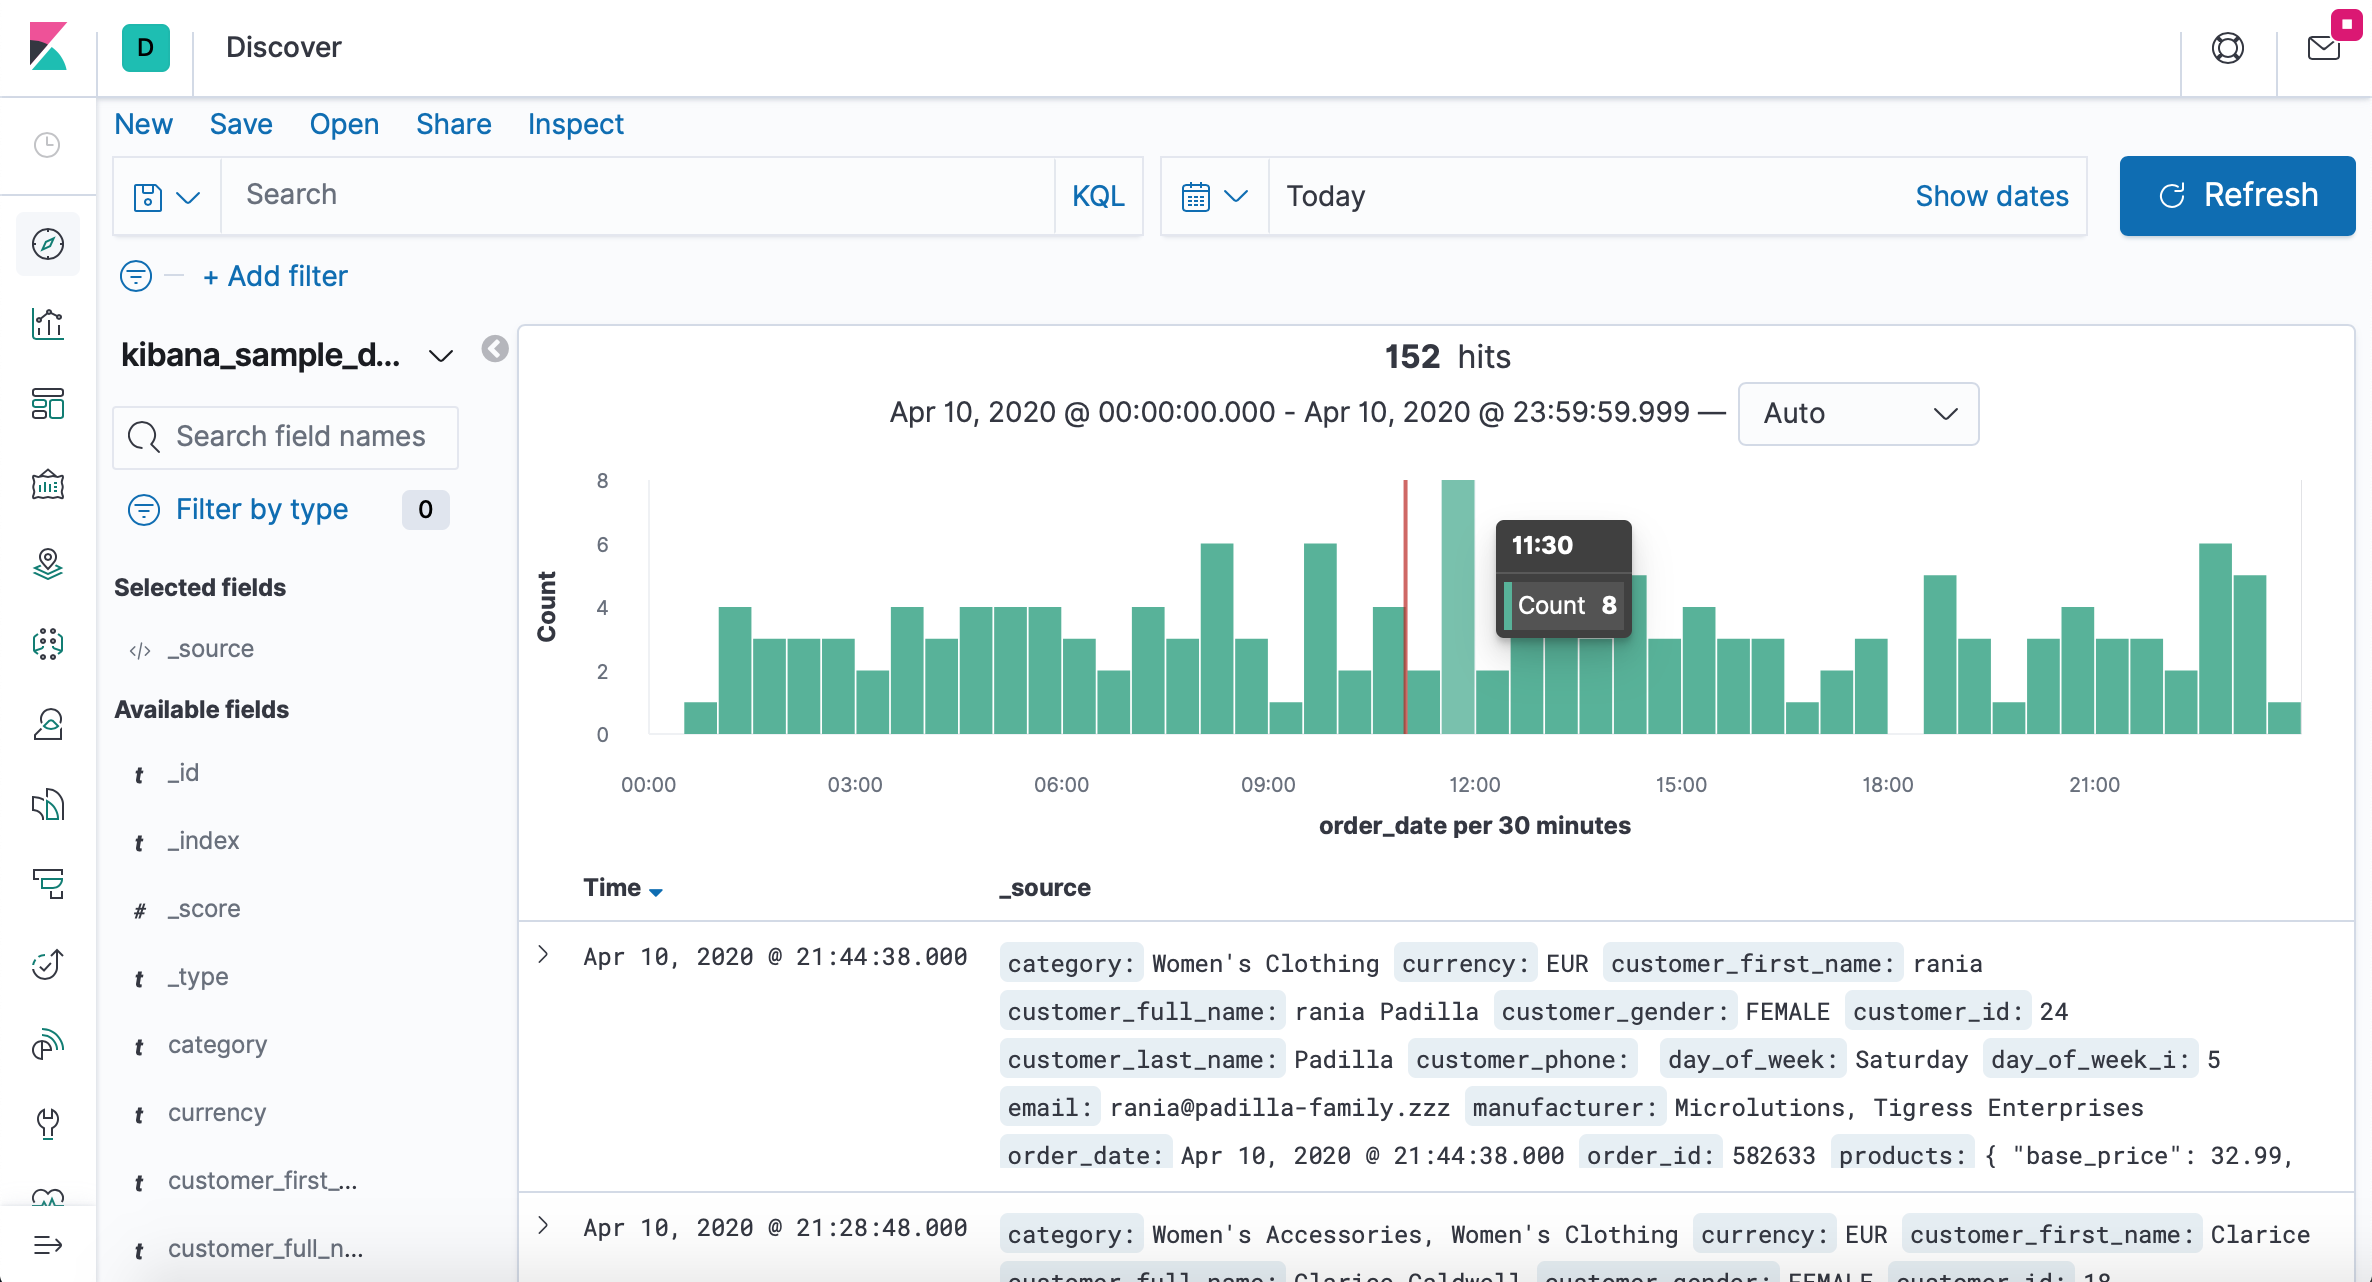
\includegraphics[width=12cm, keepaspectratio]{img/development/Discover-kibana.png}
  \caption{Pestaña Discover del cliente de Kibana}
  \label{fig:kibanadiscover}
\end{figure}

Una vez que ya hemos comprendido, viéndolo en la pestaña de “Discover”, con que clase de datos trabajamos; pasaremos a ver cómo se crean las visualizaciones. Para ello, iremos a la pestaña “Visualization” y lo primero con lo que nos encontramos es con que, al habernos descargado datos de prueba, ya vienen unas predeterminadas. Antes de ponernos a probar a crear una, lo mejor será coger una de estas predeterminada para entender su funcionamiento.

Esta visualización nos muestra una gráfica tipo Pie que viene configurada para que nos muestre el número de ventas en base al género del cliente, ya sea hombre (MALE) o mujer (FEMALE). A mano izquierda vemos que existe también un editor que nos permite configurar la gráfica. Existen dos pestañas dentro de la misma:

\begin{itemize}
    \item \underline{Data:} donde configuraremos qué datos queremos que nos muestre, separados entre metrics y buckets (que explicamos más adelante).
    \item \underline{Options:} como su propio nombre indica, configuraciones opcionales. Por ejemplo, en este caso te permite indicarle donde se desea colocar la leyenda, o si queremos que la gráfica sea rellena o no.
\end{itemize}

\begin{figure}[H]
  \centering
  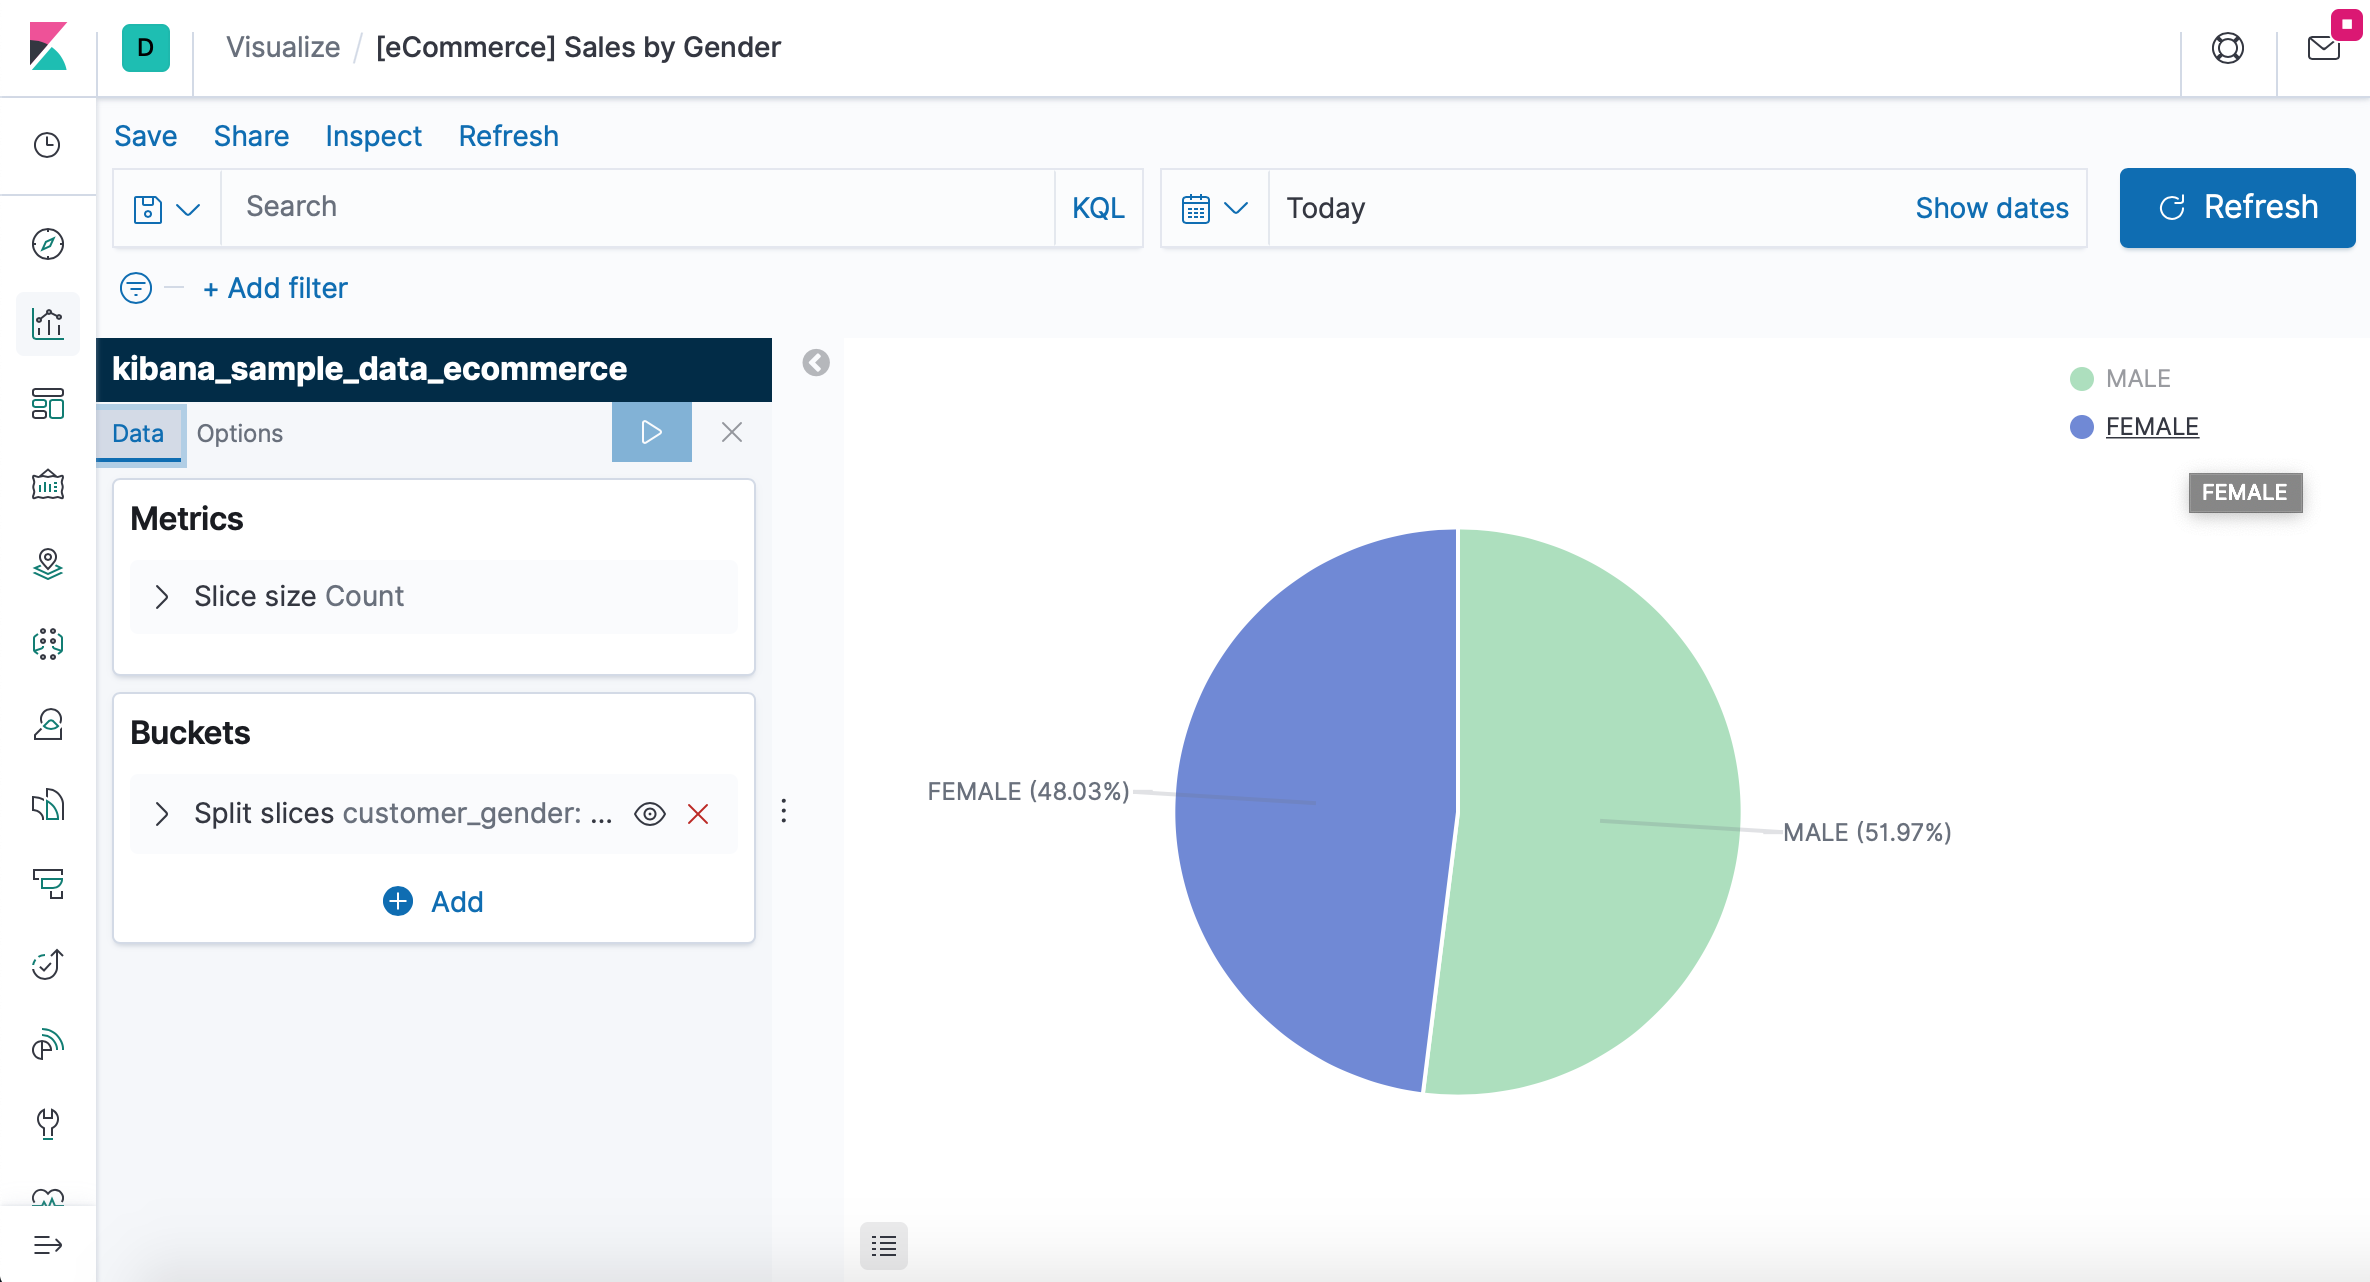
\includegraphics[width=12cm, keepaspectratio]{img/development/Kibana-visualization-pie.png}
  \caption{Visualizacion Pie en el cliente de Kibana}
  \label{fig:kibanapie}
\end{figure}

Ahora que ya entendemos un poco el funcionamiento de las visualizaciones, pasaremos a crear una propia; pero que sea diferente de la anterior. Por ejemplo, nos interesa ver desde qué países se han realizado las ventas. Elegimos “Create Visualization” y seleccionamos, para este caso, la visualización tipo Table. 

Como no nos queremos complicar mucho, lo único que haremos será pedirle que nos muestre la cantidad de ventas que se han realizado en base a los países. Para ello, vamos en la pestaña “Data” y en metrics le indicamos “Count” que nos mostrará la cantidad de ventas. Y luego “Buckets” que nos los clasifique por país. Para ello, se ha de seleccionar en “Aggregations” la opción de “Terms” y luego en “Field” le indicamos que queremos que sea por nombre de país “geoip.region\_name”. Además, nos permite que lo podamos ordenar de mayor a menor o viceversa; o que solo nos muestre, por ejemplo, los 5 primeros. O incluso, darle una etiqueta a los datos que estamos mostrando.

\begin{figure}[H]
  \centering
  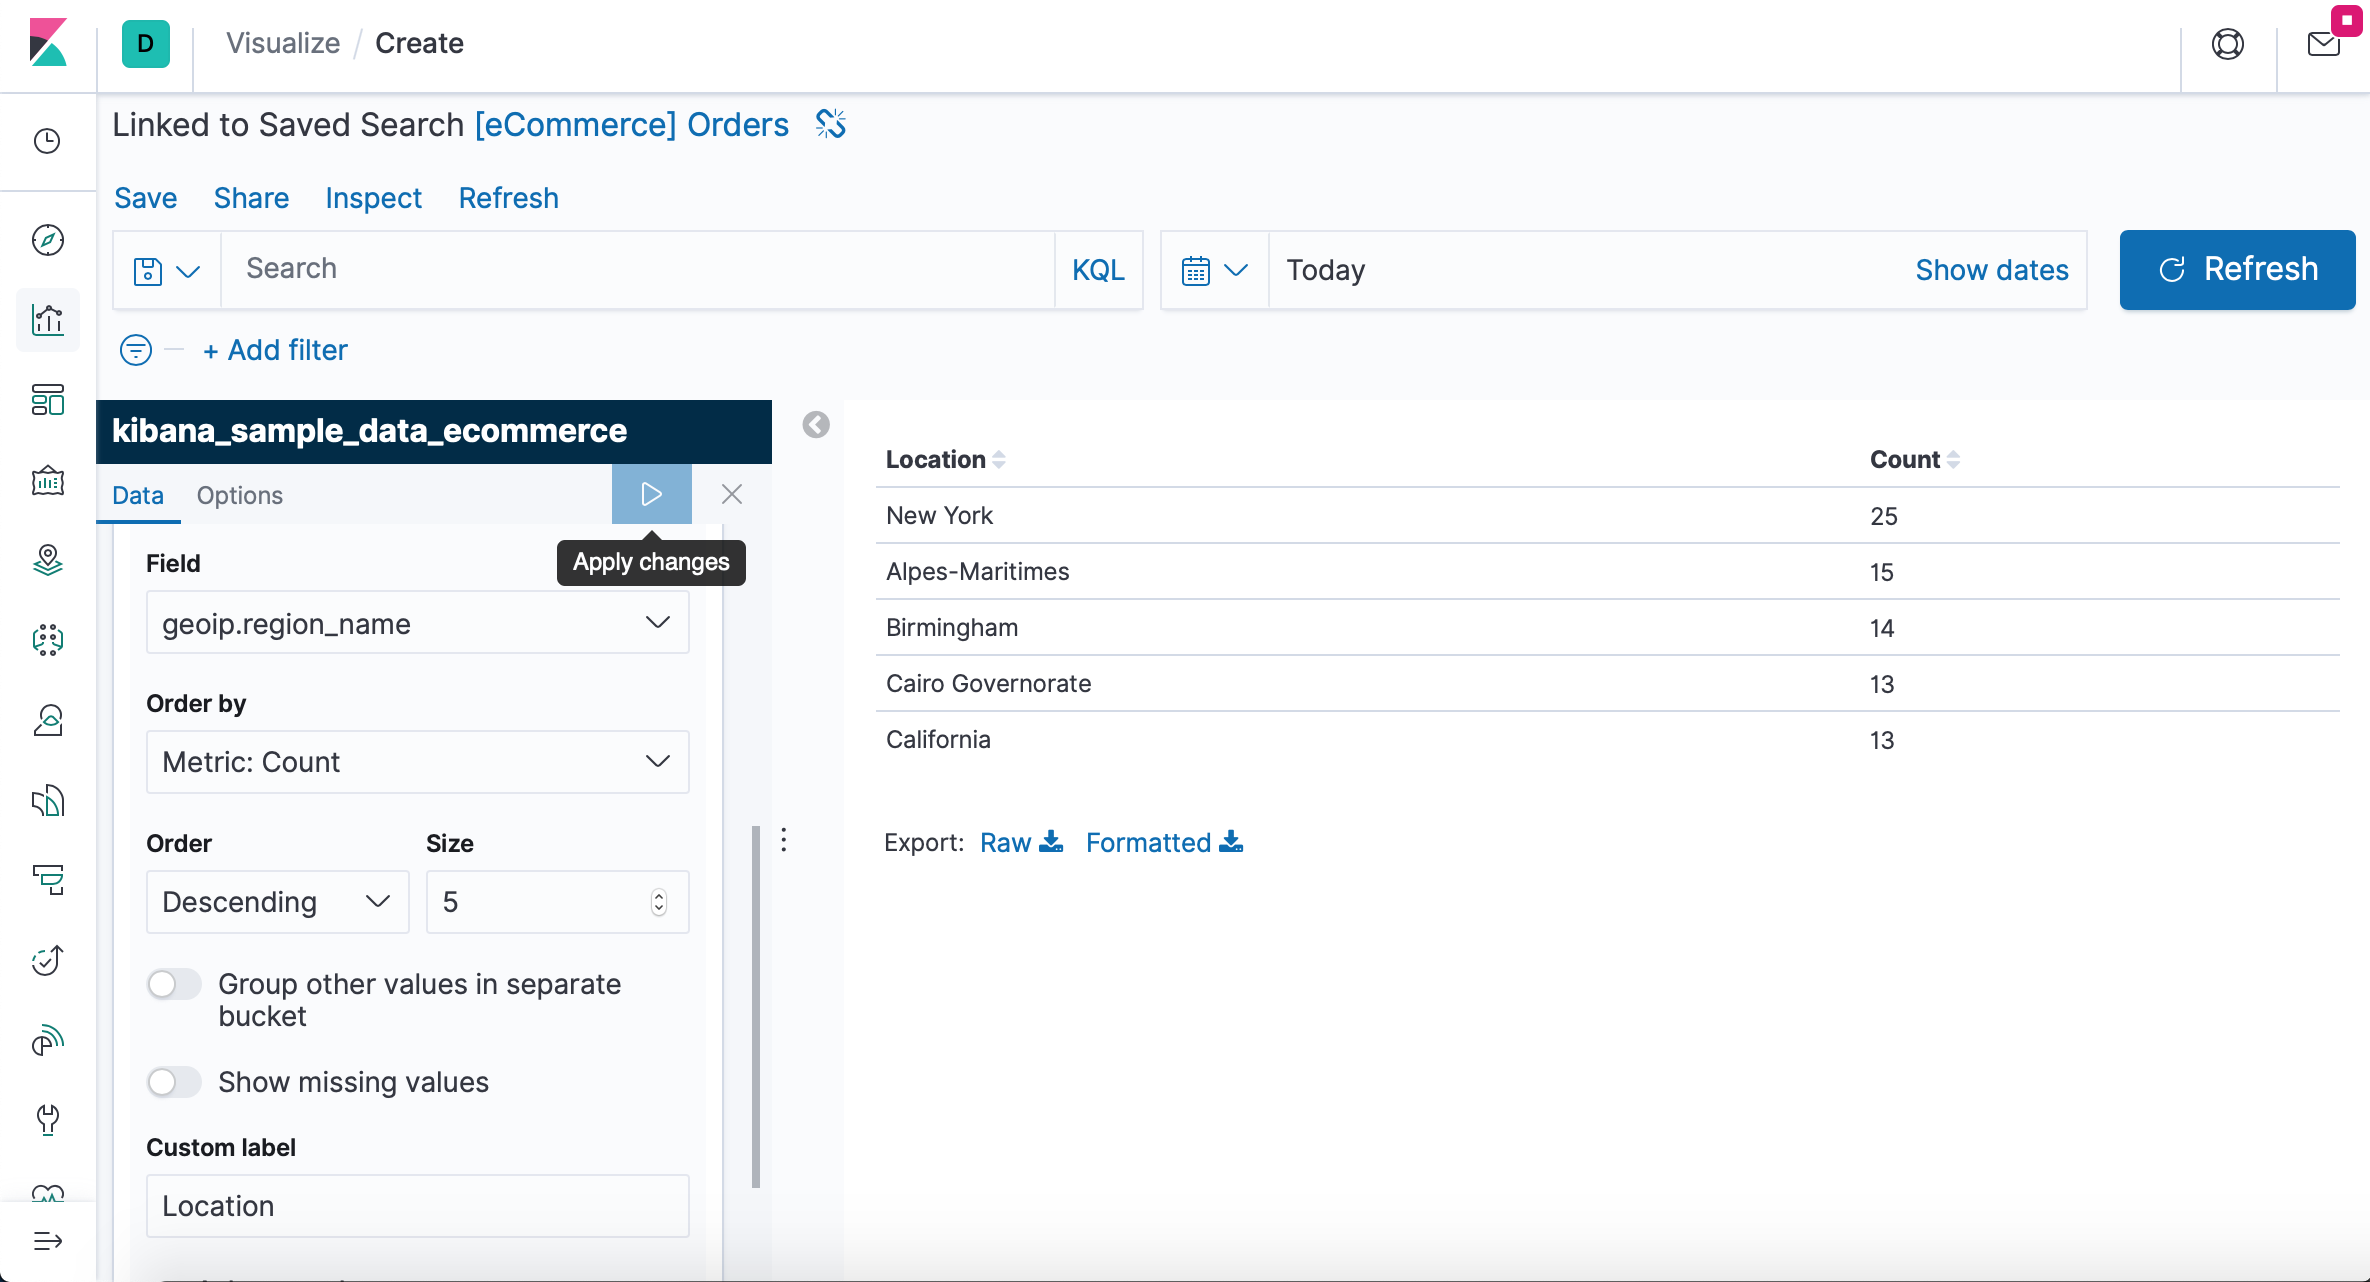
\includegraphics[width=12cm, keepaspectratio]{img/development/kibana-table-editor.png}
  \caption{Creación de Vizualización Table en el cliente de Kibana}
  \label{fig:kibanatable}
\end{figure}

Una vez seleccionado cómo queremos nuestra visualización, solo tenemos que darle a “Apply changes” y se actualizará al instante. Y una vez que tengamos la visualización que queremos, simplemente la guardamos dándole a “Save”.

Después de haber probado alguna visualización y haber creado una propia, nos interesa conocer otra sección interesante y es la que encontramos en la pestaña “Dashboard”. En esta, nos encontramos con que ya existe una predeterminada así que, aunque podemos crear una nueva, la editaremos.

Para entenderlo bien, la dashboard nos muestra en una misma página todas las visualizaciones que tenemos creadas y que queremos que sean mostradas. Lo que nos permite en edición es añadir o eliminar visualizaciones, colocarlas en un sitio u otro; o incluso darles el tamaño que nos interese.

\begin{figure}[H]
  \centering
  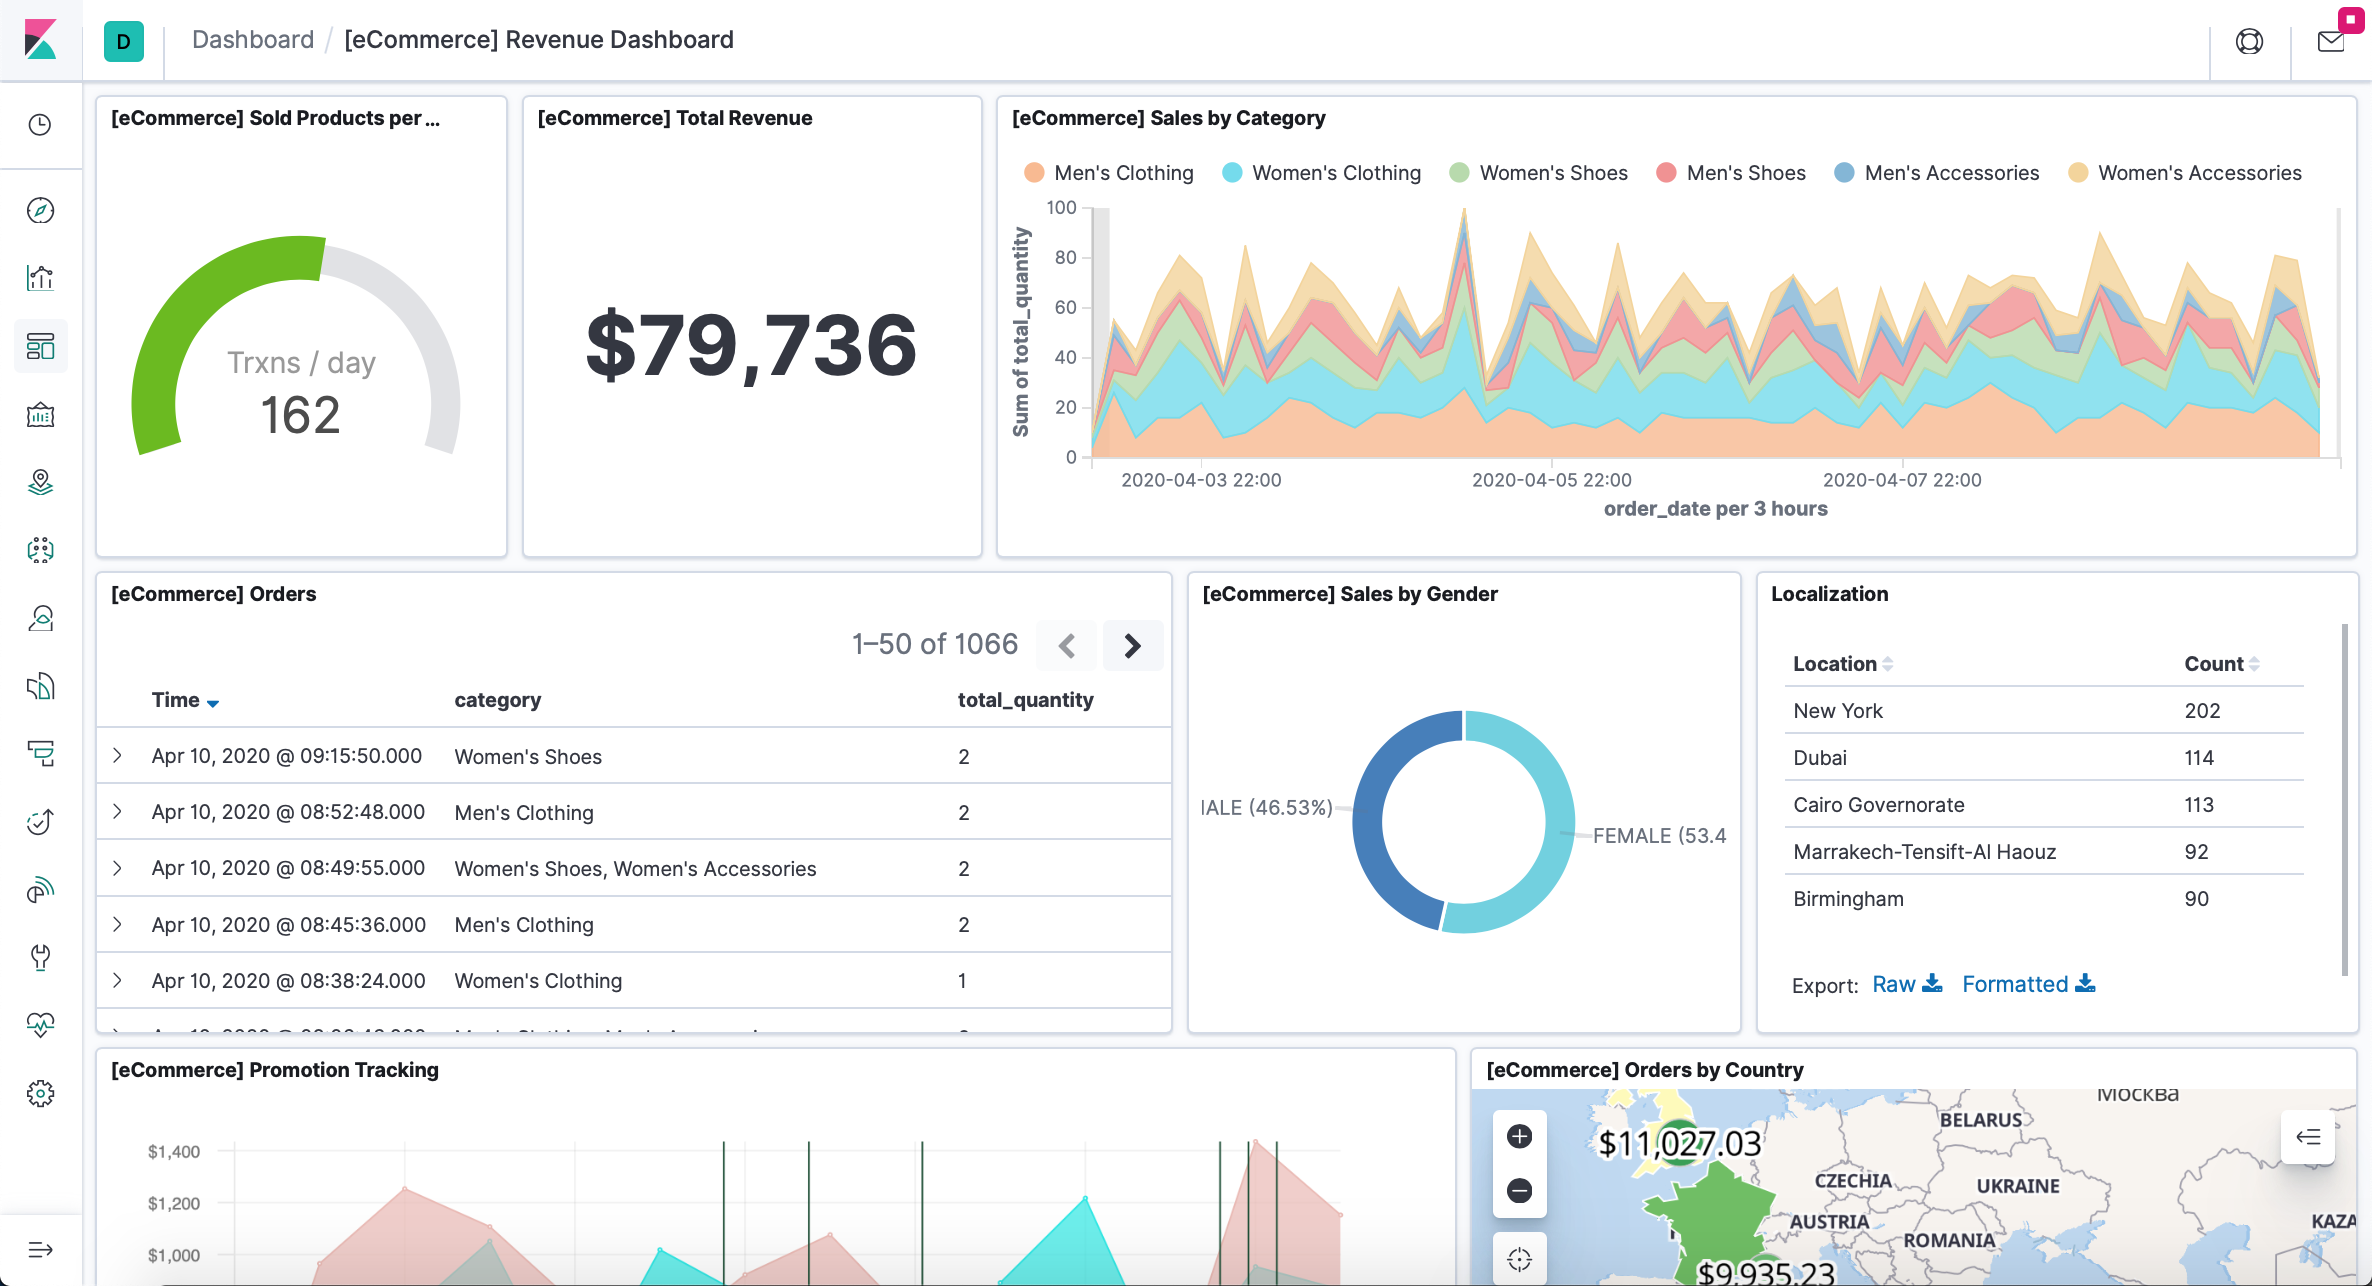
\includegraphics[width=12cm, keepaspectratio]{img/development/kibana-dashboard.png}
  \caption{Dashboard en el cliente de Kibana}
  \label{fig:kibanadashboard}
\end{figure}


%CREANDO ENTORNO DE DESARROLLO
\subsection{Creando el Entorno de Desarrollo}

Ahora que ya entendemos un poco el funcionamiento del cliente de Kibana, pasaremos a crearnos el entorno de desarrollo que utilizaremos para crear nuestro plugin. Este nos permitirá ver en tiempo real los cambios que realicemos.

Siguiendo las indicaciones que podemos encontrar en la sección correspondiente para contribuir en el proyecto (“CONTRIBUTING.md”), dentro del repositorio de kibana.

Una vez tengamos creado nuestro entorno de desarrollo, pasaremos a documentarnos cómo se crean plugin para Kibana. Para ello, elastic no proporciona artículos en su blog de como crear unos plugins básicos. Aunque está un poco obsoleta la documentación, únicamente nos quedaremos con la parte de cómo es la estructura de ficheros.

Por el momento no vamos a detallar el contenido de los ficheros (lo explicaremos más adelante), simplemente nos enfocaremos en qué función tiene cada uno.

Lo primero que haremos será crear un directorio con en nombre de nuestro plugin en “KIBANA\_HOME/plugins”. Dentro de esta habrá dos ficheros:

\begin{itemize}
    \item \underline{package.json:} un simple fichero para npm donde le indicamos el nombre de nuestro plugin, version, autor, etc. Y sobretodo, las dependencias que necesitamos que nos instale para poder utilizarlas en nuestro proyecto.
    \item \underline{index.js:} este es el módulo principal. En él registramos nuestro plugin indicando el tipo de plugin (dentro de kibana) que es, visualización en este caso; y hacemos referencia al fichero principal.
\end{itemize}

A esto le sigue crear un nuevo directorio con el nombre “public/” que contendrá todos los ficheros de nuestro plugin (controllers, configurations, templates, etc). Antes hemos dicho que desde “index.js” hacíamos referencia a el fichero principal de nuestro plugin, pues es aquí donde lo crearemos.

\begin{itemize}
    \item \underline{public/plugin-name.js:} para el caso de las visualizaciones es donde registramos las diferentes visualizaciones, puede ser una o varias, que vamos a añadir en kibana a través de nuestro plugin.
\end{itemize}

Todos los ficheros anteriormente mencionados son los principales para el funcionamiento de esto; pero a mayores se le pueden añadir más ficheros. Algunos ejemplos opcionales:

\begin{itemize}
    \item \underline{public/plugin-name-controller.js:} como su propio nombre indica, sería el controlador de nuestro plugin. En el contiene toda la parte lógica de nuestra visualización.
    \item \underline{public/plugin-name.html:} template del plugin.
    \item \underline{public/plugin-name.less:} hoja de estilo del plugin.
    \item \underline{public/options-template.html:} template para la pestaña “options” del editor.
\end{itemize}

De forma más visual, podemos decir que la estructura de ficheros para crear un plugin para kibana es la siguiente:


\begin{lstlisting}[frame=single]
KIBANA_HOME/plugins/
|___plugin-name/
    |___package.json
    |___index.js
    |___public/
        |___plugin-name.js
        |___plugin-name-controller.js
        |___plugin-name.html
        |___plugin-name.less
        |___options-template.html

\end{lstlisting}



%TESTEANDO BIBLIOTECA PARA LAS VISUALIZACIONES
\subsection{Testeando Biblioteca para las Visualizacione}

Al igual que necesitamos conocer el funcionamiento de kibana, también necesitamos tener unos conceptos básicos sobre los componente visuales que vamos a incorporar para nuestras visualizaciones para kibana.

La opcion de usar Babiaxr ha sido muy acertada, ya que permite crear gráficas, a partir de datos proporcionados, dentro de un escenario webVR. Así que antes de nada, analizaremos lo que nos ofrece y cómo se crean.

Dentro del repositorio de babiaxr podemos ver los distintos tipos de componentes que tienen creados. Dichas componentes han sido creadas a partir del framework a-frame (ver ...).

Lo primero que haremos será probar los diferentes componentes que tienen: “geopiechart”, “geosimplebarchar”, “geo3dbarchart” y “geobubblechart”. Todas ellas se pueden probar desde su web.

\begin{figure}[H]
  \centering
  \minipage{0.32\textwidth}
  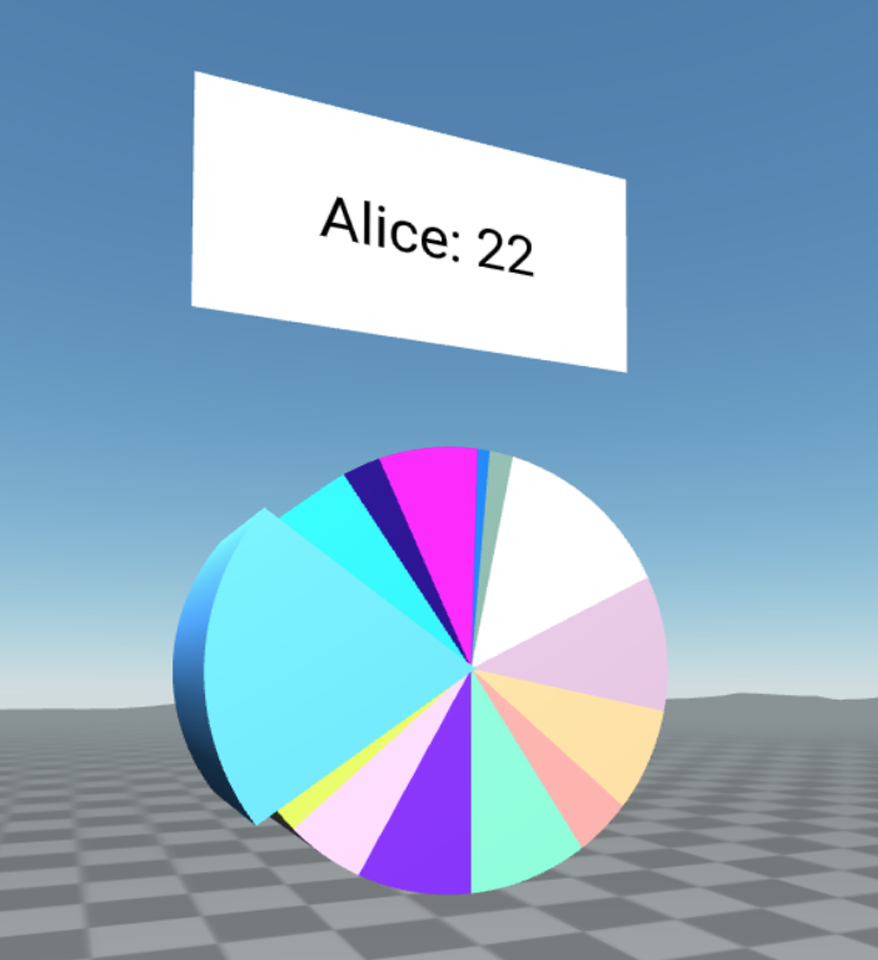
\includegraphics[width=5cm, keepaspectratio]{img/development/babiaxr-pie.png}
  \caption{Geopiechart}
  \label{fig:babiaxrgeopiechart}
  \endminipage\hfill
  \minipage{0.32\textwidth}
  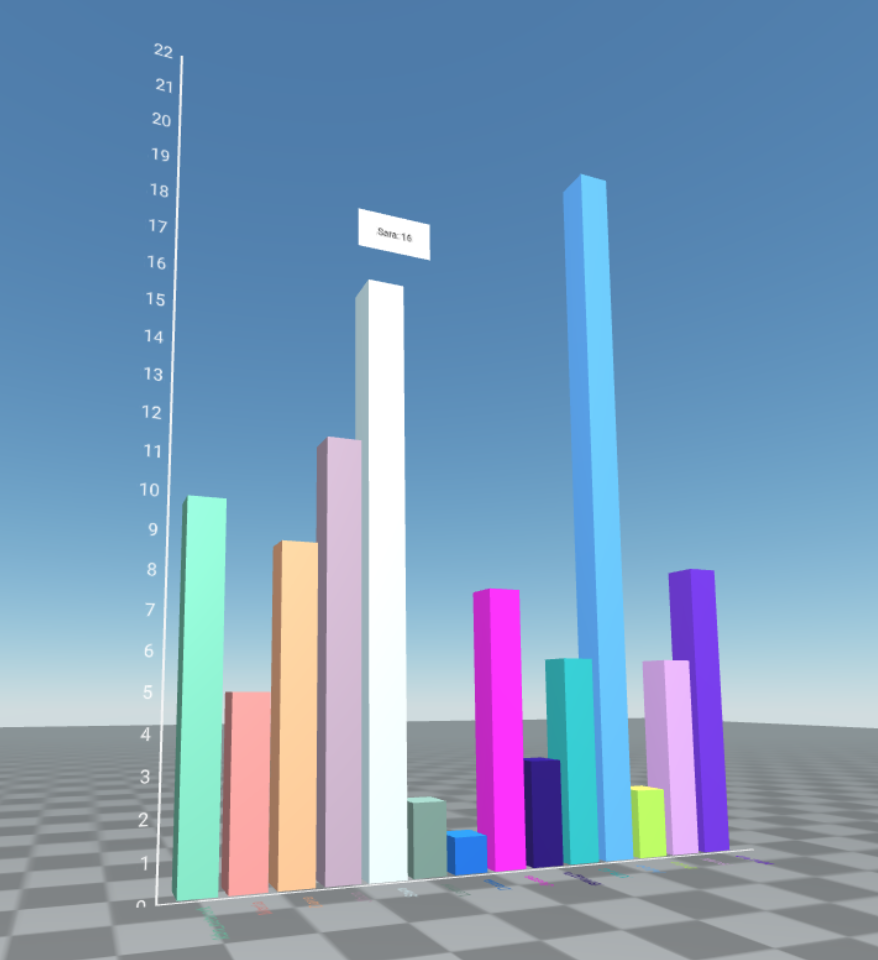
\includegraphics[width=5cm, keepaspectratio]{img/development/babiaxr-simplebar.png}
  \caption{Geosimplebarchart}
  \label{fig:babiaxrgeosimplebarchart}
  \endminipage\hfill
  \minipage{0.32\textwidth}
  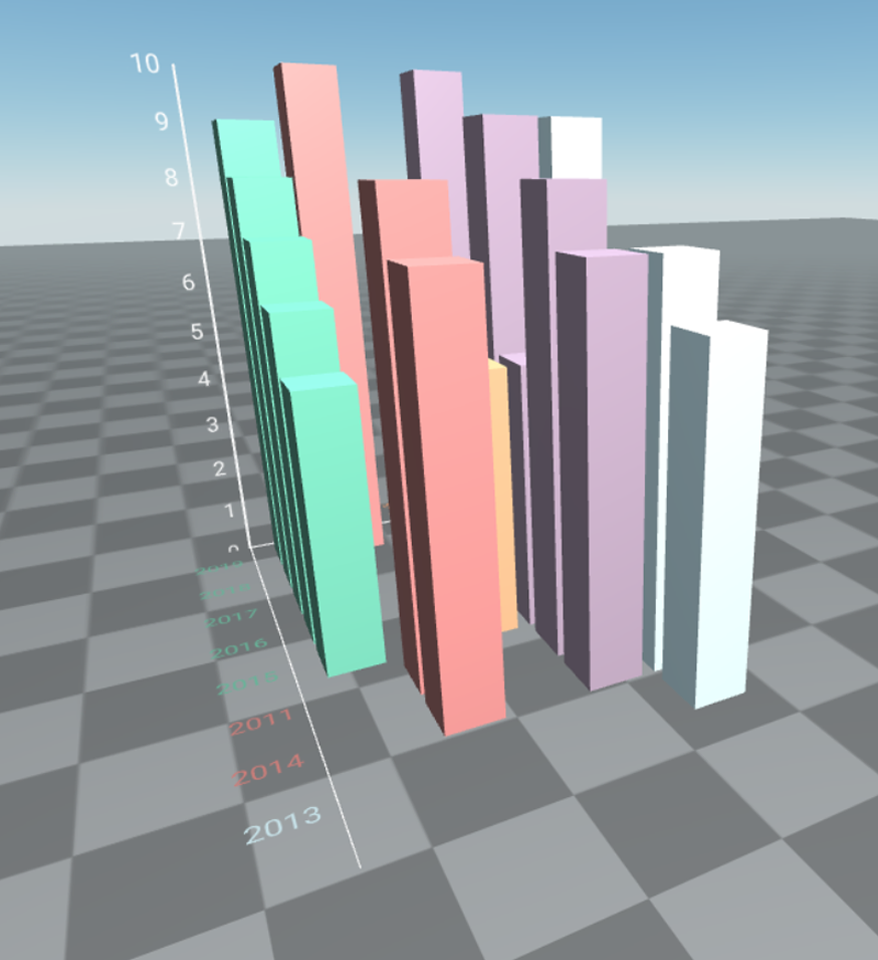
\includegraphics[width=5cm, keepaspectratio]{img/development/babiaxr-3dbar.png}
  \caption{Geo3dbarchart}
  \label{fig:babiaxrgeo3dbarchart}
  \endminipage\hfill
\end{figure}

\begin{figure}[H]
  \centering
  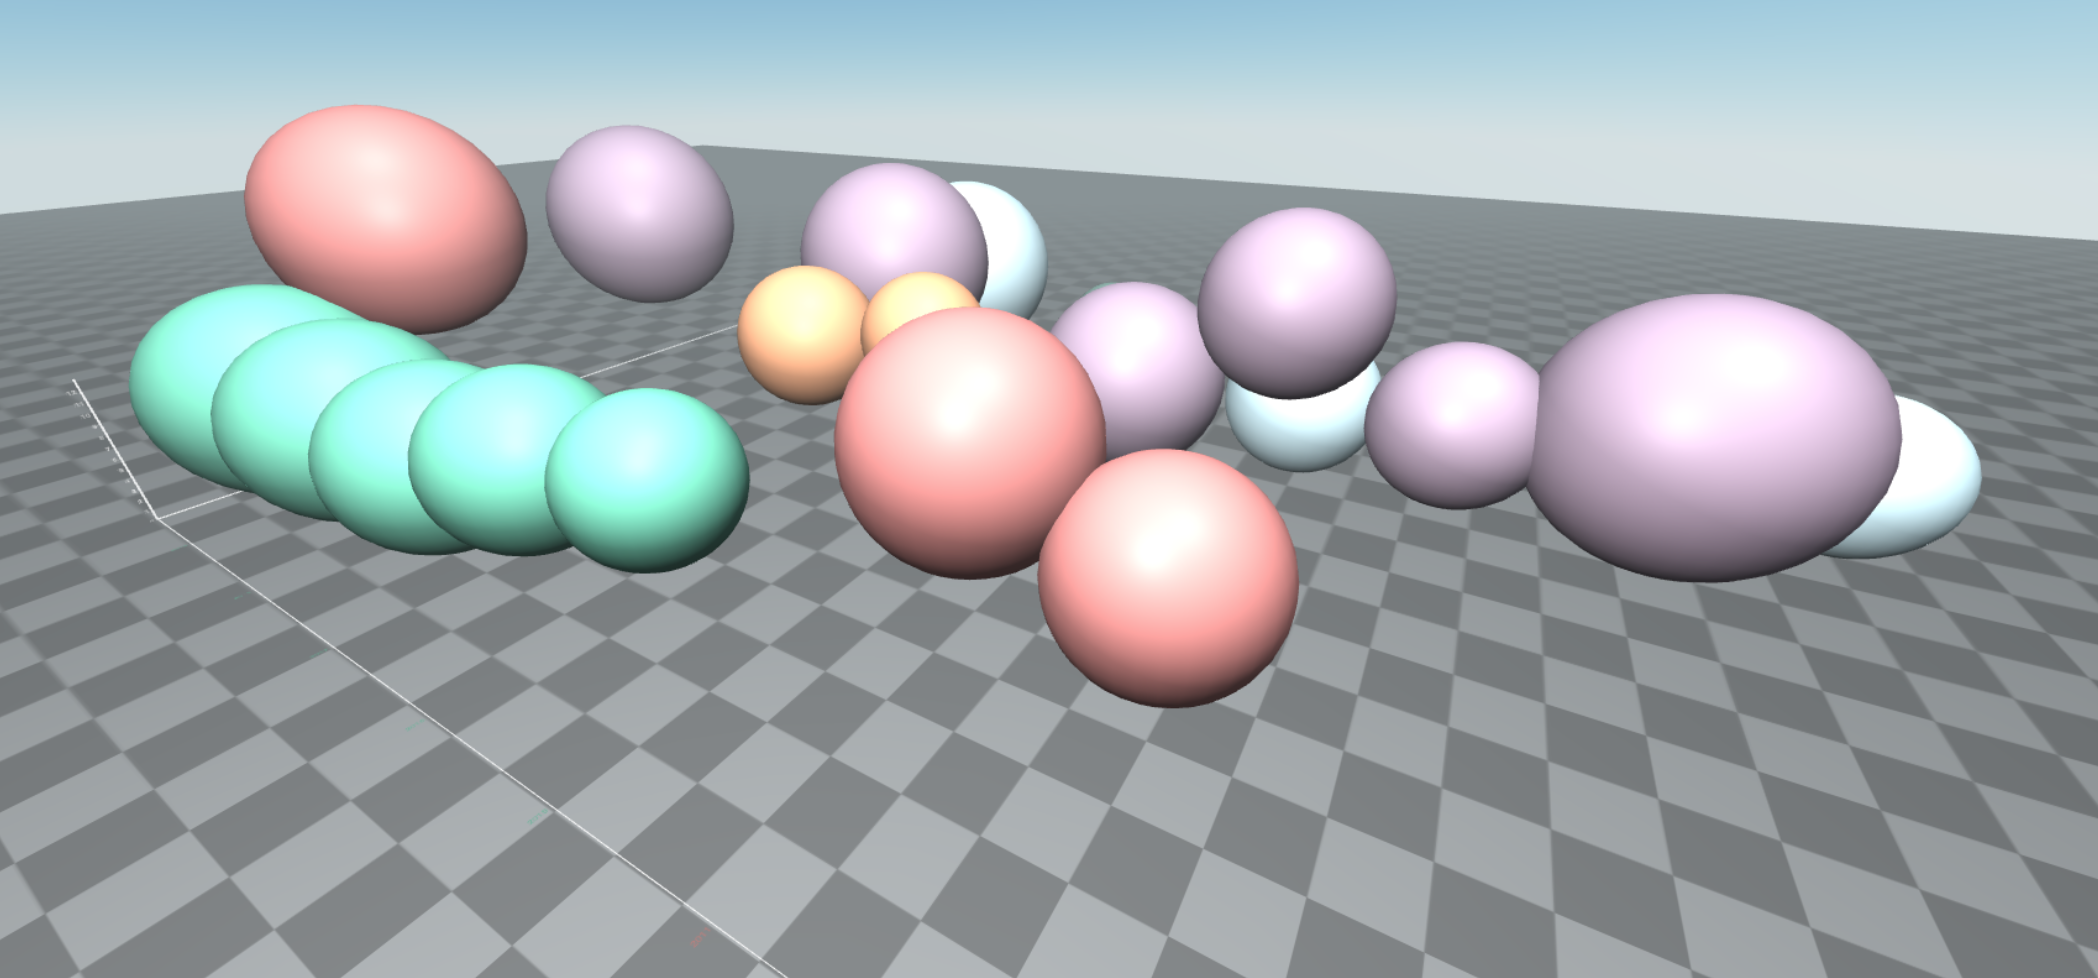
\includegraphics[width=10cm, keepaspectratio]{img/development/babiaxr-bubble.png}
  \caption{Geobubblechart}
  \label{fig:babiaxrgeobubblechart}
\end{figure}


Una vez que hemos visto lo que hace, probaremos a crear nuestro propio escenario con la componente “geopiechart” con datos que le daremos de forma manual. Para ello, nos apoyaremos en la documentación que nos facilita su autor.

\begin{lstlisting}[frame=single]
<a-entity geopiechart='legend: true;
    data: [{"key":"Andrea","size":9},{"key":"URJC","size":8},
    {"key":"ETSIT","size":7},{"key":"kibana","size":6},
    {"key":"elasticsearch","size":5},{"key":"Jesus","size":8},
    {"key":"David","size":7}]'
position="-3 5 15" rotation="90 0 0"></a-entity>

\end{lstlisting}

Obteniendo como resultado:

\begin{figure}[H]
  \centering
  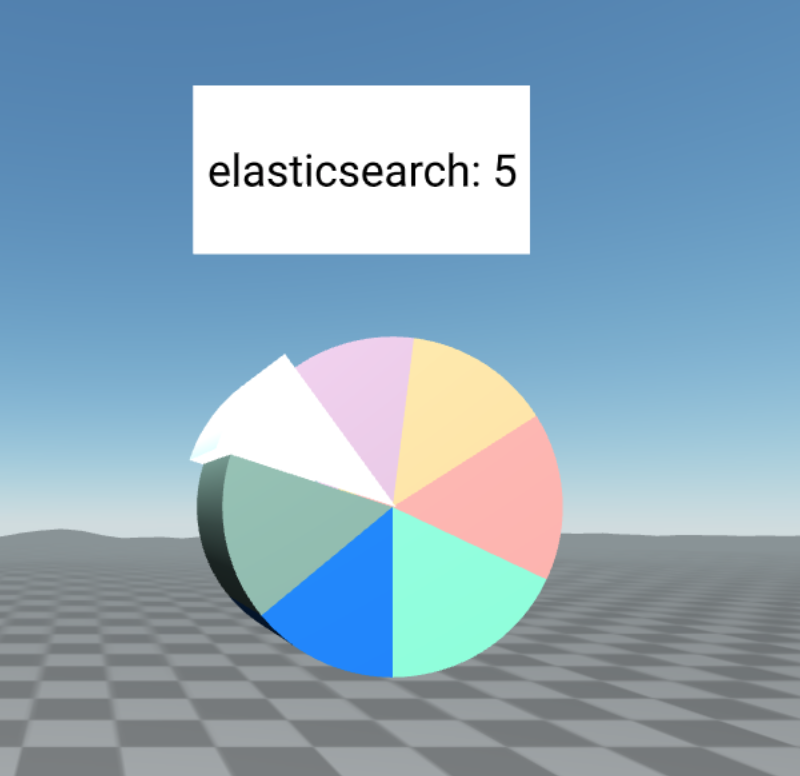
\includegraphics[width=6cm, keepaspectratio]{img/development/prueba-babiaxr.png}
  \caption{Pie Chart de Prueba}
  \label{fig:pruebababiaxr}
\end{figure}

Con todo esto, ya podemos proceder a crear nuestro primer plugin.


%%%%%%%%%%%
% SPRINT 1
%%%%%%%%%%%

\section{Sprint 1: Primeros Plugins de Visualización }
\label{sec:sprint1}

Ahora que conocemos las herramientas con las que trabajamos, es hora de ponernos a crear nuestro primer plugin. Esta parte es vital para el aprendizaje, así que iremos paso a paso.

Lo primero que haremos será crear un plugin simple, sin usar datos, que nos muestre un “Hola Mundo” como visualización. Esto nos ayudará a conocer más en profundidad el funcionamiento  de la estructura anteriormente explicada.

Una vez que hayamos conseguido crear este primer plugin, intentaremos implementar una figura creada con a-frame. Esto nos ayudará a entender cómo podemos añadir componentes a-frame a nuestras visualizaciones.

También intentaremos crear un componente sencillo de a-frame y lo implementaremos. Esto nos ayudará a entender cómo se han creado los componentes de babiaxr.

En resumen:
\begin{enumerate}
    \item Crearemos un plugin de visualización sin datos.
    \item Implementaremos A-frame sin usar datos.
    \item Crearemos un componente A-Frame y lo implementaremos.
\end{enumerate}

\subsection{Plugin Simple sin Datos}
Anteriormente (ver Capítulo) explicamos cómo era la estructura base para crear plugins para Kibana. Iremos parte por parte hasta conseguir tener una visualización que simplemente nos muestre un “Hola Mundo”.

A este primer plugin lo llamaremos “hello-world-vis” y comenzaremos a programar los primeros archivos que nos permitirá registrar el plugin e instalar las dependencias npm que necesitamos.

\begin{lstlisting}[frame=single]
{
  "name": "hello-world-vis",
  "version": "0.0.1",
  "kibana": {
    "version": "kibana"
  }
}
\end{lstlisting}

Parámetros utilizados:
\begin{itemize}
    \item \underline{name}: nombre del plugin.
    \item \underline{version}: versión de nuestro plugin.
    \item \underline{kibana}: versión de kibana.
\end{itemize}

Como solo es una versión de prueba, únicamente indicaremos el nombre del plugin, la versión y para que version de kibana es. Esta última se debe indicar bien, sino no funcionará. Por eso, como estamos desarrollando para la version 7.6, esto tiene que venir reflejado en nuestro “package.json”. En esta ocasión, al ser un simple hola-mundo no necesitaremos instalar ninguna dependencia.

Ahora procederemos a registrar nuestro plugin en “index.js”:

\begin{lstlisting}[frame=single]
export default function (kibana) {
  return new kibana.Plugin({
    uiExports: {
      visTypes: [
        'plugins/hello-world-vis/hello-world-vis'
      ]
    }
  });
}
\end{lstlisting}

Parámetros utilizados:
\begin{itemize}
    \item \underline{uiExports}: indica que el tipo de modulo vamos a exportar. Dentro de esta existen varios tipos: (hacks, visTypes, fieldformats, etc).
    \item \underline{vis\_Types}: indicamos que el módulo que vamos a exportar se trata de un plugin de visualización.
\end{itemize}

Una vez dentro de “vis\_Types” indicaremos el directorio donde se encuentra el archivo principal de nuestro plugin “public/hello-world-vis.js”. Ahora pasaremos a crearlo. Al igual que para los plugins, las visualizaciones también deben registrarse. 

Lo primero que haremos será importar el paquete dentro de kibana que nos permitirá registrar nuestra visualización. Debido a la migración que se está realizando en kibana, la documentación que facilitaban y cualquier otro tutorial estaban obsoletos. Por lo que se tuvo que realizar una extensa búsqueda entre el repositorio de kibana en github y sus issues para ver cómo era la nueva forma de registrar las visualización. 

Al final, la mejor forma de averiguarlo fue inspeccionar dentro del código de kibana y ver cómo registraban las visualizaciones que vienen de forma predeterminada en el cliente de kibana. Esta se encuentra en el fichero “kibana/src/legacy/core\_plugins/kbn\_vislib\_vis\_types/public/ kbn\_vislib\_vis\_types.js”, y la usaremos de base para la forma de registrar nuestras futuras visualizaciones.

Con esto, ya podemos importar el paquete que nos permitirá registrar la visualización:

\begin{lstlisting}[frame=single]
import { setup as visualizations } from '../../../src/legacy/
core_plugins/visualizations/public/np_ready/public/legacy';
\end{lstlisting}

Ahora pasaremos a definir nuestra visualización:
\begin{lstlisting}[frame=single]
// define the new visualization
const helloWordDefinition = {
    name: 'hello_world_vis',
    title: 'Hello World',
    icon: 'visBarVertical',
    description: 'Hola mundo',
    visualization: hello_world_Controller,
    editor: 'default',
}
\end{lstlisting}

Parámetros utilizados:
\begin{itemize}
    \item \underline{name}: nombre de nuestra visualización.
    \item \underline{title}: título que aparecerá en el menú para elegir nueva visualización.
    \item \underline{icon}: icono que aparecerá en dicho menú.
    \item \underline{description}:  descripción que aparecerá en dicho menú.
    \item \underline{visualization}: indicaremos el controlador que usaremos en la visualización, éste lo crearemos a continuación para exportarlo.
    \item \underline{editor}: añade el editor, pero como por ahora no nos interesa, lo dejaremos en ‘default’.
\end{itemize}

Y por último, registramos la visualización:

\begin{lstlisting}[frame=single]
//Register the provider with the visType Register
visualizations.types.createBaseVisualization
(helloWordDefinition);
\end{lstlisting}

Ya tenemos registrada nuestra primera visualización. Lo que le sigue es crear el controlador donde estará toda la parte lógica de nuestro plugin, pero antes de comenzar con ella vamos a crear un pequeño template “public/index.html”, con el contenido de la visualización, que no es más que un “Hola Mundo”.

\begin{lstlisting}[frame=single]
<div class='Hello world'>
    <p>!`Hola Mundo!</p>
</div>
\end{lstlisting}

Listo esto, comenzamos a crear nuestro controlador “public/hello-world-controller.js”. Lo primero que haremos será importar nuestro template.

\begin{lstlisting}[frame=single]
import template from './index.html'
\end{lstlisting}

Este controlador es una clase con su correspondiente constructor; pero también necesitará las funciones de “render()” y “destroy()” para funcionar. Comenzamos creando el constructor:

\begin{lstlisting}[frame=single]
// define class
class VisController {
   constructor(el, vis) {
      console.log('Creating...');
      this.el = el;
      this.vis = vis;

      this.container = document.createElement('div');
      this.container.className = 'myvis-container-div';
      this.el.appendChild(this.container);
   }
\end{lstlisting}

Lo único que hacemos es coger las variables el y vis y crear un container:

\begin{itemize}
    \item \underline{el}: contenido de la visualización.
    \item \underline{vis}: contiene los parámetros que se crean al registrar la visualización.
    \item \underline{container}: en este contenedor añadiremos todo lo que queremos que muestre la visualización.
\end{itemize}

A continuación crearemos la función “destroy()” que destruirá la visualización cada vez que salimos de la visualización o cada vez que actualizamos los datos que se van a mostrar en la visualización.

\begin{lstlisting}[frame=single]
destroy() {
  this.el.innerHTML = '';
  console.log('Destroying...');
}
\end{lstlisting}

Y por último, creamos la función “render()”.

\begin{lstlisting}[frame=single]
render(visData, status) {
  if (visData) {
    this.container.innerHTML = template;
  }
};
\end{lstlisting}

Como Kibana es un cliente que permite monitorizar los datos almacenados en elasticsearch, al crear un visualización se espera que kibana realice una petición a elasticsearch con los datos que quiere mostrar; y éste los devuelva. Estos datos vienen en dentro de la variable “visData”,; por tanto actualizaremos nuestra visualización cada vez que recibamos datos, aunque en esta ocasión los datos estarán en blanco. 
Lo único que haremos es meter el template que anteriormente hemos creado en el container de la visualización.

El siguiente paso es exportar el controlador:

\begin{lstlisting}[frame=single]
export { VisController };
\end{lstlisting}

E importarlo en “public/hello-world-vis.js”:

\begin{lstlisting}[frame=single]
import { VisController } from './hello-world-controller.js';
\end{lstlisting}

Como resultado nos encontramos con que dentro de crear nueva visualización aparece nuestra visualización con su nombre, icono y descripción.

\begin{figure}[H]
  \centering
  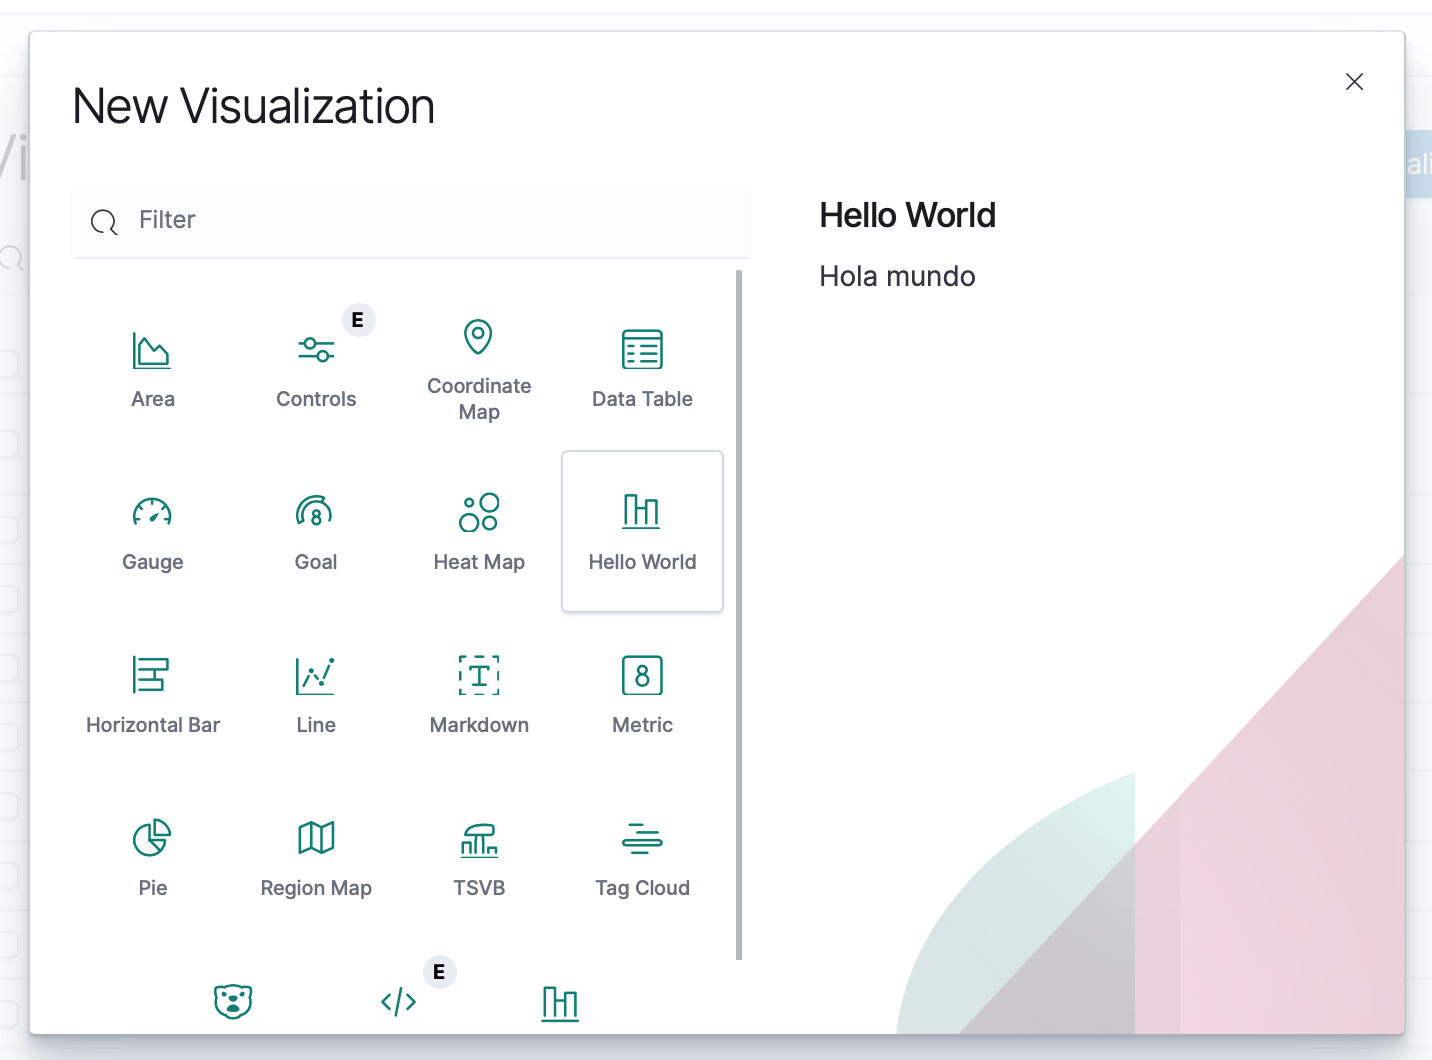
\includegraphics[width=10cm, keepaspectratio]{img/development/menu-visualizaciones.png}
  \caption{Menú con la nueva visualización}
  \label{fig:menuvisualization}
\end{figure}

Y obteniendo como resultado nuestra visualización “Hola Mundo!”.

\begin{figure}[H]
  \centering
  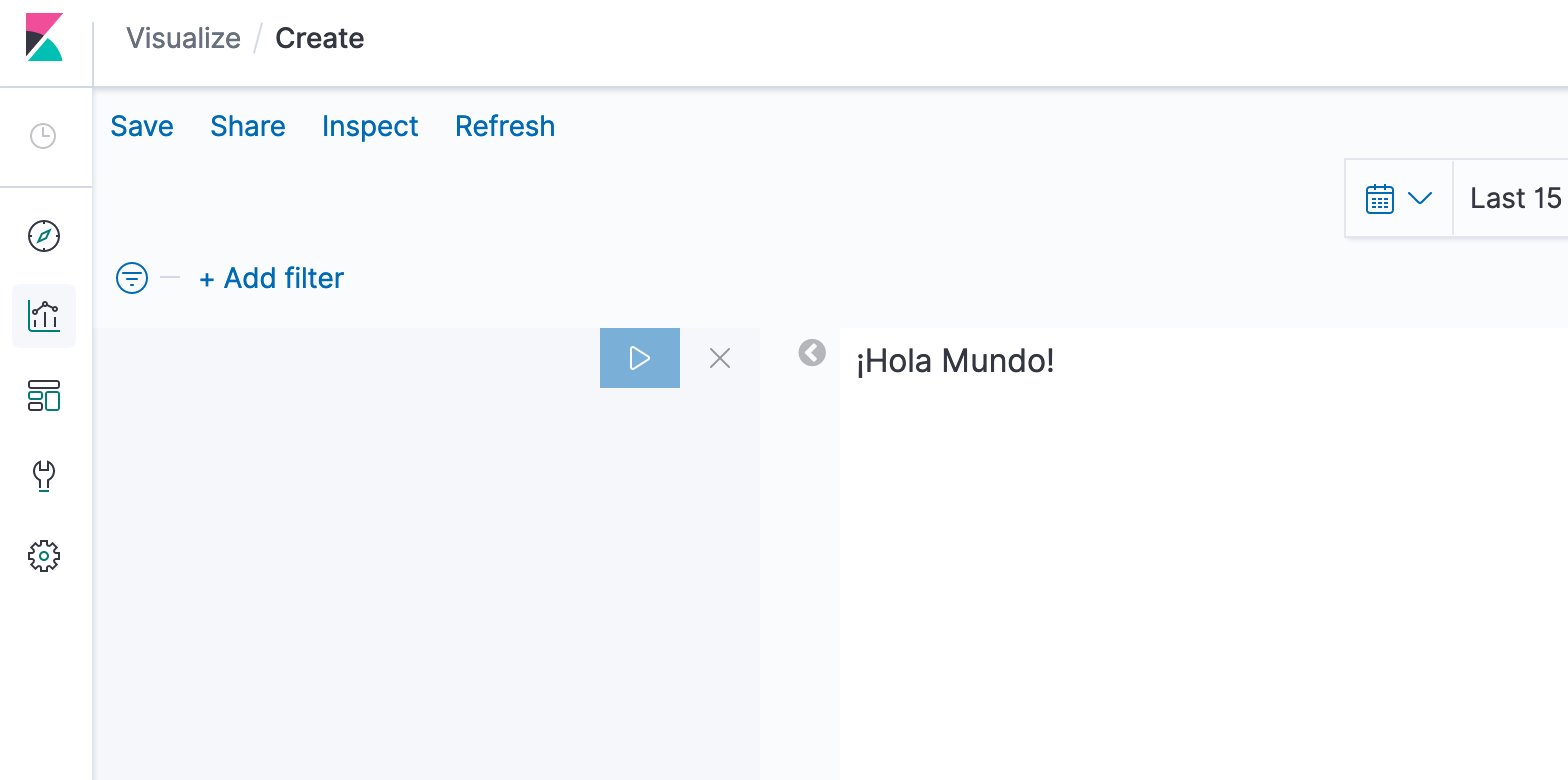
\includegraphics[width=10cm, keepaspectratio]{img/development/resultado-hola-mundo.png}
  \caption{Resultado Visualización "Hola Mundo"}
  \label{fig:resultadoholamundo}
\end{figure}

\subsection{Implementación de A-Frame sin Datos}

Una vez aprendidas las bases de cómo se crea un plugin de visualización para Kibana, el siguiente paso será conseguir integrar algún componente de la biblioteca de a-frame para comprobar si estas dos tecnologías son compatibles entre sí.

En esta situación crearemos una visualización, tomando como base el plugin “hello-world-vis” que creamos anteriormente; y le intentaremos añadir un componente primitivo de la biblioteca de a-frame (por ejemplo, un cubo).

Para esto, necesitaremos tener instalado previamente el módulo npm de a-frame. Esto se consigue añadiendo las dependencias en “package.json”.

\begin{lstlisting}[frame=single]
"dependencies": {
"aframe": "^0.9.2"
}
\end{lstlisting}

Y  para instalarlo usaremos el comando “npm install” dentro del directorio que contiene nuestro “package.json”.

Una vez que hemos descargado e instalado el módulo de a-frame, lo declaramos en el controlador de la visualización “hello-world-controller.js” para que podamos usarlo en el template.

\begin{lstlisting}[frame=single]
//import aframe
const aframe = require('aframe');
\end{lstlisting}

Y modificamos el HTML del template “index.html” para que dibuje un cubo con a-frame. Para ello, debemos conocer al menos estas dos etiquetas: 

\begin{itemize}
    \item \underline{a-scene}: permite manejar elementos creados con THREE.js y WebVR. Todos estos elementos deben estar contenido en esta etiqueta, sino no funcionará. Salvo que se le declare, creará por defecto la cámara y las luces.
    \item \underline{a-box}: crea un componente cubo en 3D según los atributos que le indiquemos.
\end{itemize}

\begin{lstlisting}[frame=single]
<a-scene>
  <a-box position="-1 0.5 -3" rotation="0 45 0"
  color="#4CC3D9"></a-box>
</a-scene>
\end{lstlisting}

Obteniendo como resultando la siguiente visualización:

\begin{figure}[H]
  \centering
  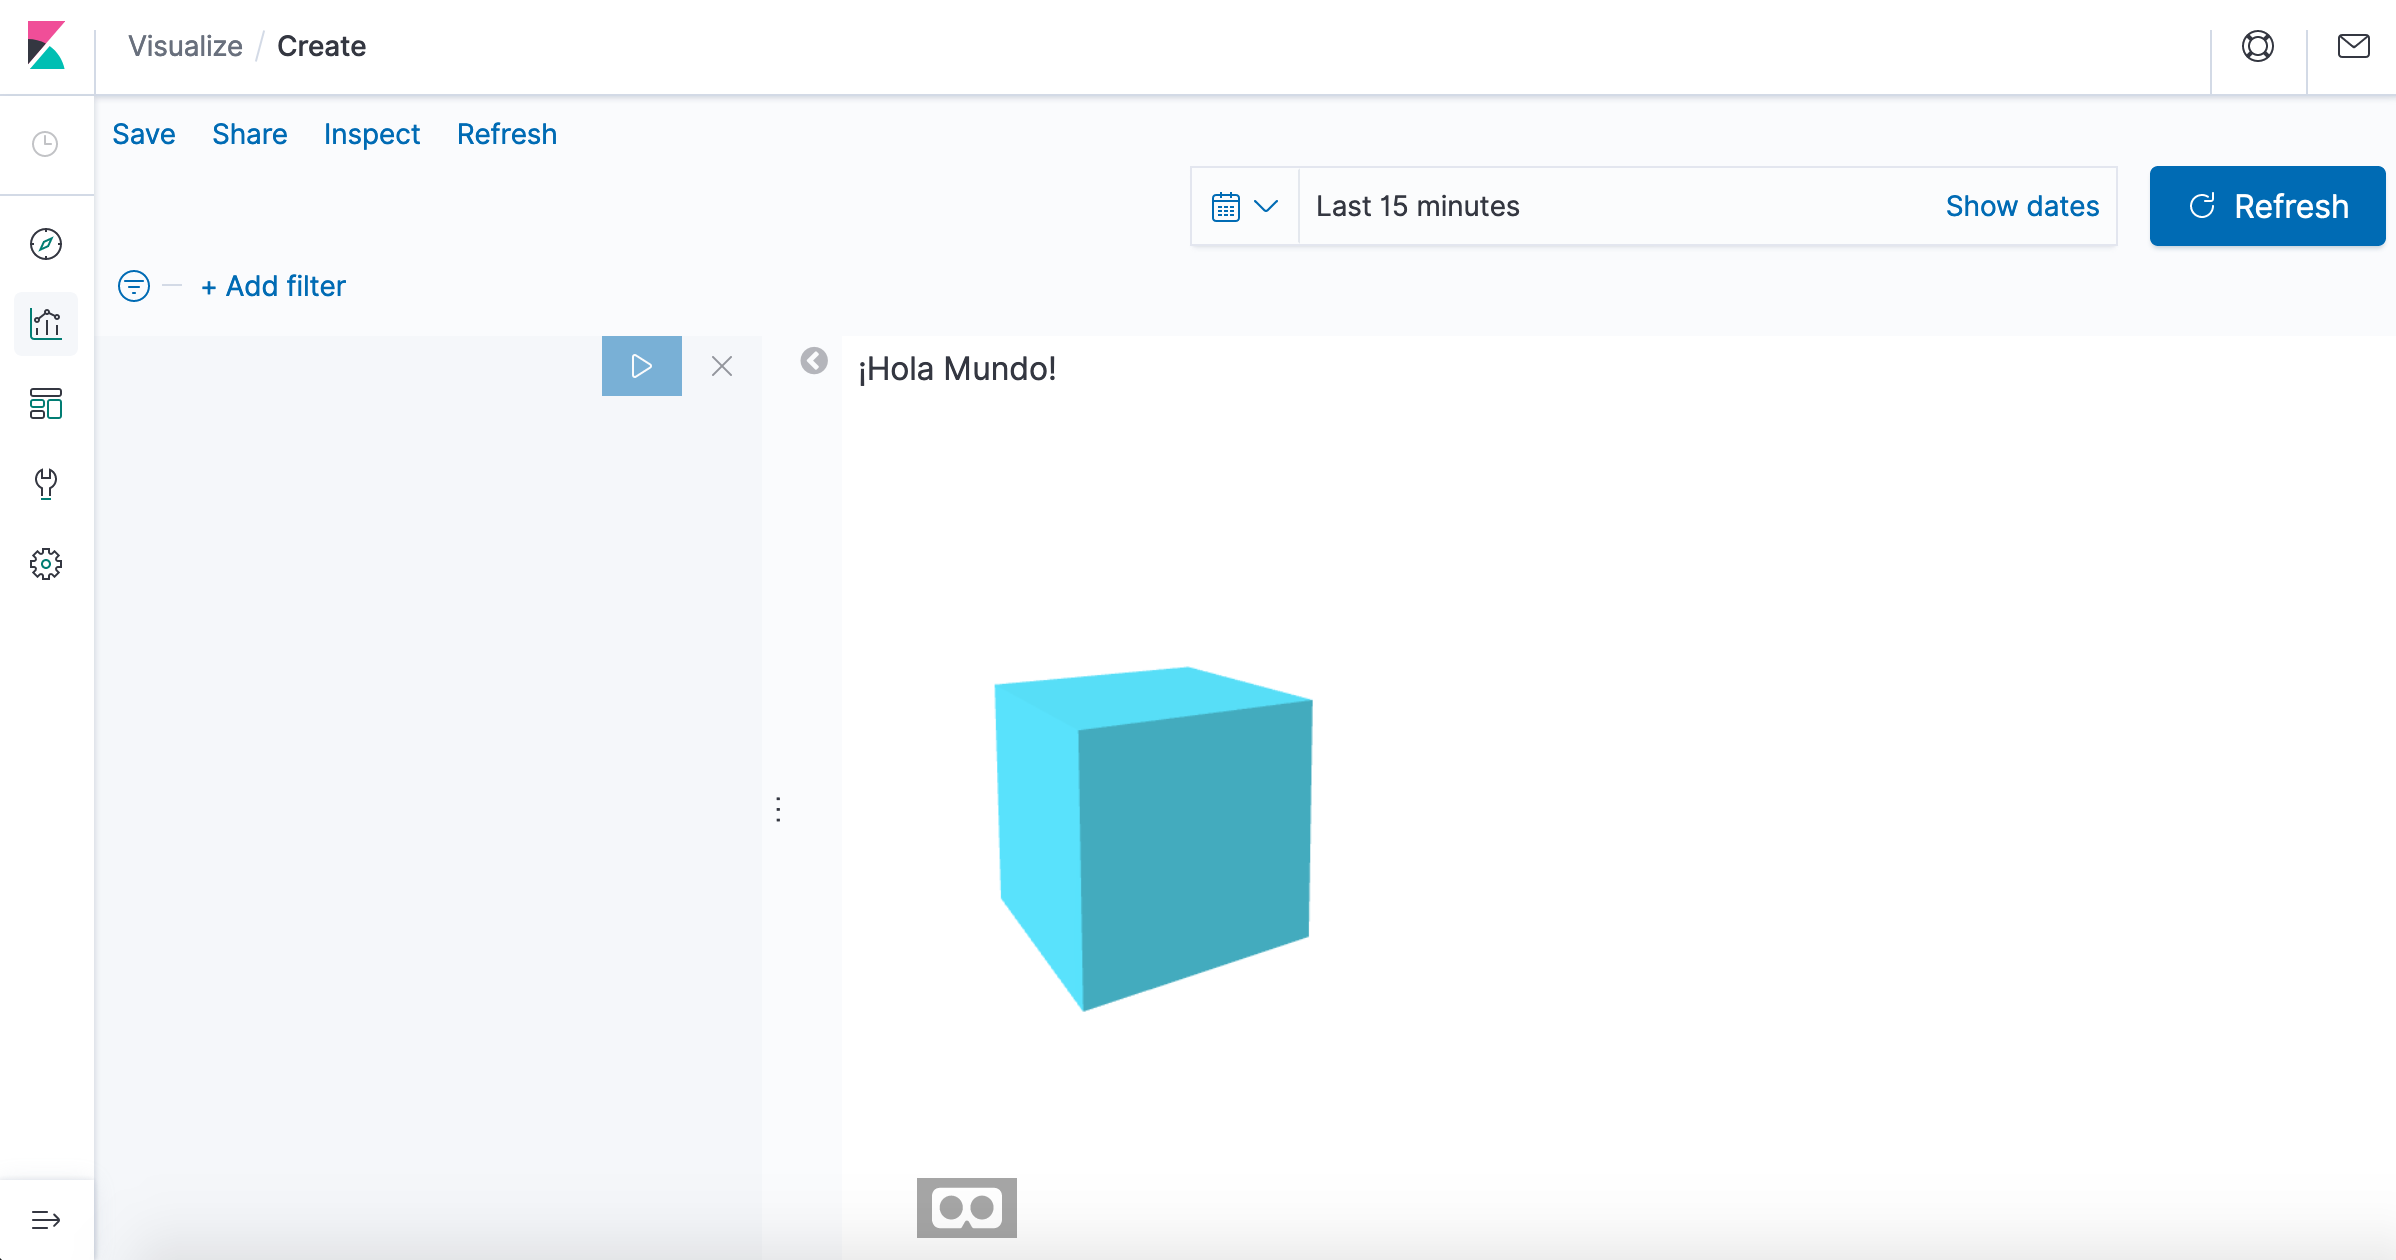
\includegraphics[width=10cm, keepaspectratio]{img/development/resultado-aframe-box.png}
  \caption{Resultado Visualización de cubo con A-frame son Datos}
  \label{fig:resultadoaframesindatos}
\end{figure}

Con esto podemos asegurar que Kibana soporta visualizaciones creadas con la biblioteca a-frame.

\subsection{Creación de Componente A-Frame}

Ahora ya sabemos que kibana nos permite usar a-frame en sus visualizaciones, pero vamos a estudiarlo más en profundidad. Como se explicó anteriormente (ver cap), BabiaXR es una biblioteca de componente creadas con a-frame; por lo que en esta ocasión se creará un componente a-frame para entender mejor el funcionamiento interno de babiaXr.

Ya que hemos creado un cubo como componente primitivo, esta vez lo sustituiremos por otro cubo; pero creado por este método tomando como referencia el ejemplo que nos facilita la documentación de a-frame. 

El primer paso es crear un fichero que se llamará “box.js” y registrar el componente de la siguiente esquema:

\begin{lstlisting}[frame=single]
// Registro de la componente
AFRAME.registerComponent('box', {
  schema: {
    width: {type: 'number', default: 1},
    height: {type: 'number', default: 1},
    depth: {type: 'number', default: 1},
    color: {type: 'color', default: '#AAA'}
  },
\end{lstlisting}

Los parámetros que le indicamos en el constructor son las propiedades que, más adelante, indicaremos dentro de las etiquetas del HTML.

Estas componentes funcionan como clases y deben contener ciertas funciones para que se puedan renderizar: init(), update(), destroy()

Comenzaremos creando la función “init()”

\begin{lstlisting}[frame=single]
 //Funcion inicial
  init: function () {
    var data = this.data;
    var el = this.el;

    // Crea la figura
    this.geometry = new THREE.BoxBufferGeometry(data.width, 
    data.height, data.depth);

    // Se le da un material
    this.material = new THREE.MeshStandardMaterial({
    color: data.color});

    // Creamos la mesh
    this.mesh = new THREE.Mesh(this.geometry, this.material);

    // Creamos el objeto 3D
    el.setObject3D('mesh', this.mesh);
  },
...
});
\end{lstlisting}

Esta función inicializa la geometría, material y malla del componente a partir de los parámetros que recibe cuando se declaran en el HTML. Para luego renderizar la figura inicializada.

La función “update()” se ejecutará cuando algún dato cambia. En este caso no lo vamos a necesitar pero como más adelante vamos a extraer datos de elasticsearch para modificar el componente, lo creamos.

\begin{lstlisting}[frame=single]
 // En caso de que los datos cambien, actualizamos la figura
  update: function (oldData) {
    var data = this.data;
    var el = this.el;

    // If `oldData` is empty, then this means we're in the 
    initialization process.
    // No need to update.
    if (Object.keys(oldData).length === 0) { return; }

    // Geometry-related properties changed. Update the geometry
    if (data.width !== oldData.width ||
        data.height !== oldData.height ||
        data.depth !== oldData.depth) {
      el.getObject3D('mesh').geometry = new 
      THREE.BoxBufferGeometry(data.width, data.height,
      data.depth);
    }

    // Material-related properties changed. Update the material
    if (data.color !== oldData.color) {
      el.getObject3D('mesh').material.color = new THREE.Color(
      data.color);
    }
  },
\end{lstlisting}

Esta función lo que hará será modificar nuestro cubo con los nuevos valores recibidos.

Y por último, creamos la función “destroy()” que borrará la figura al cerrar la visualización.

\begin{lstlisting}[frame=single]
// Borramos la figura
remove: function () {
this.el.removeObject3D('mesh');
}
\end{lstlisting}

Ahora que ya tenemos creada una componente propia, lo que sigue es declararla en nuestro controlador.

\begin{lstlisting}[frame=single]
import './box.js'
\end{lstlisting}

Y modificar el template para que nos dibuje un cubo creado con nuestra componente; y le añadiremos también una esfera con la etiqueta <a-sphere> para ver que se pueden mezclar componentes primitivas de a-frame con componente creadas por otros usuarios. 

Para insertar estas componentes, que no vienen de forma pre-determinadas por a-frame, usaremos la etiqueta <a-entity> seguido del atributo con el nombre de la componente tal y como se ha registrado. En nuestro caso <a-entity box></a-entity>.

\begin{lstlisting}[frame=single]
<a-scene embeded>
    <!-- Figura cubo por componente aframe  -->
    <a-entity box="width: 0.5; height: 0.25; depth: 1; 
        color: #4CC3D9" position="-1 0.5 -3" 
        rotation="0 45 0"></a-entity>
    <!-- Figura esfera basica de aframe -->
    <a-sphere position="0 1.25 -5" radius="1.25" 
        color="#EF2D5E" shadow></a-sphere>
</a-scene>
\end{lstlisting}

Una de las complicaciones que no se mencionaron anteriormente fue que la escena se salía de la visualización de kibana. Añadiendo el atributo embedded a la escena corregimos este error; pero para asegurarnos haremos una pequeña hoja de estilos para que el <div> de nuestra visualización no se salga, la cual llamaremos “hello-world.less”.

\begin{lstlisting}[frame=single]
.myvis-container-div {
  width: 100%;
}
\end{lstlisting}

Y la importamos en el controlador de la visualización.

\begin{lstlisting}[frame=single]
import style from './aframe.less';
\end{lstlisting}

Obteniendo como resultado la siguiente visualización:

\begin{figure}[H]
  \centering
  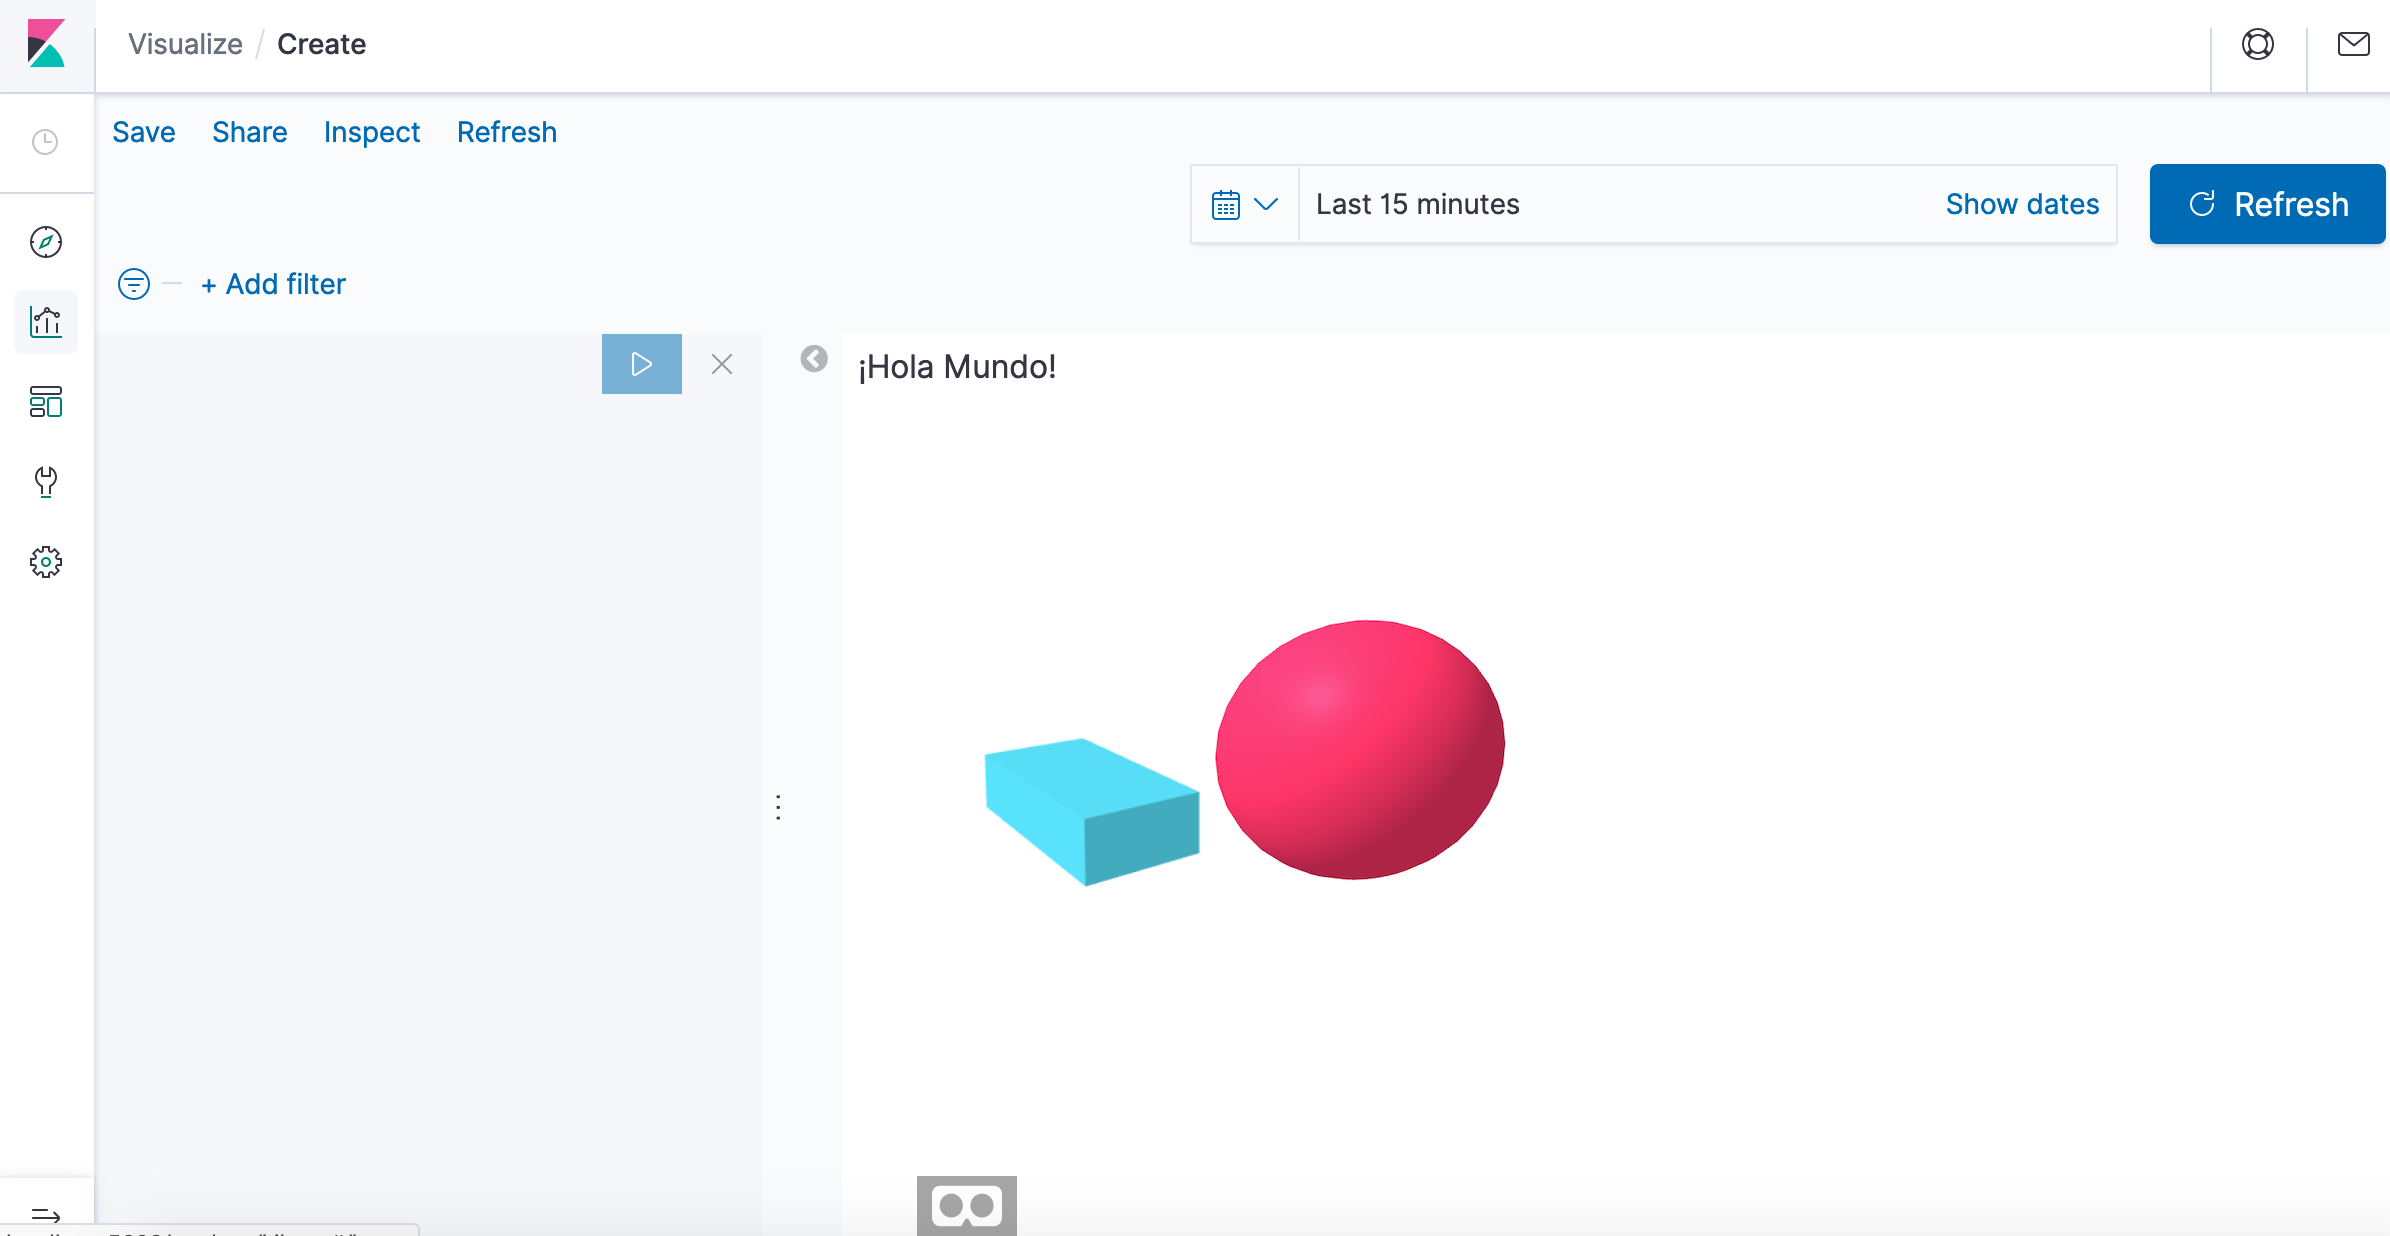
\includegraphics[width=10cm, keepaspectratio]{img/development/resultado-componente-box.png}
  \caption{Resultado Visualización de componente cubo con Esfera de A-frame sin Datos}
  \label{fig:resultadocomponente}
\end{figure}




%%%%%%%%%%%
% SPRINT 2
%%%%%%%%%%%

\section{Sprint 2: Visualización con datos Elasticseach }
\label{sec:sprint2}

Hasta este punto hemos aprendido a crear un plugin simple para kibana e integrarlo con aframe. El siguiente paso será aprender a sacar datos de elasticsearch y poder dibujar un figura de aframe, en este caso un cubo, con las dimensiones que le obtenemos de dichos datos. Para ello, seguiremos los siguiente pasos:
\begin{enumerate}
    \item Añadir Editor y Schemas.
    \item Construir Visualización que muestre datos.
    \item Integración de Aframe con datos.
\end{enumerate}

\subsection{Editor y Schemas}

Antes de ponernos a crear una nueva visualización donde nos muestre datos de elasticsearch, necesitamos un editor que nos permita seleccionar los datos que queremos mostrar. 

Comenzaremos creando el diseño de nuestro editor. Kibana nos permite seleccionar dos tipo de datos: metrics y buckets.
\begin{itemize}
    \item \underline{metrics:}hace referencia a datos que se pueden calcular, por ejemplo, media, máximo, sumatorio, etc.
    \item \underline{buckets:}refiere a un conjunto de datos que no se pueden calcular, por ejemplo, fechas, sucursales, tipos, etc.
\end{itemize}

Como el objetivo final de este sprint es crear una visualización que nos muestre un cubo, determinamos que necesitaremos 3 datos metrics que serán los datos que usaremos para crear las dimensiones del cubo que dibujaremos más adelante.

Estos datos vienen estructurados dentro de Schemas que el propio Kibana permite declarar a la hora de crear la visualización para luego registrarla. Para ello, añadiremos las siguiente líneas en “kbn\_aframe.js”:

Antes de nada, importamos los correspondientes paquetes que nos permite declarar los schemas e indicar el tipo de dato que vamos a usar, en este caso metrics.

\begin{lstlisting}[frame=single]
import { Schemas } from 'ui/vis/editors/default/schemas';
import { AggGroupNames } from 'ui/vis/editors/default';
\end{lstlisting}

Una vez importado, añadiremos nuevos parámetros dentro de la función createBaseVisualization():

\begin{lstlisting}[frame=single]
schemas: new Schemas([
        {
          group: AggGroupNames.Metrics,
          name: 'x-axis',
          title: 'X-axis',
          min: 1,
          max: 1,
          aggFilter: ['count', 'avg', 'sum', 'min', 'max', 
          'cardinality', 'std_dev']
        },
        {
          group: AggGroupNames.Metrics,
          name: 'y-axis',
          title: 'Y-axis',
          min: 1,
          max: 1,
          aggFilter: ['count', 'avg', 'sum', 'min', 'max', 
          'cardinality', 'std_dev']
        },
        {
          group: AggGroupNames.Metrics,
          name: 'z-axis',
          title: 'Z-axis',
          min: 1,
          max: 1,
          aggFilter: ['count', 'avg', 'sum', 'min', 'max', 
          'cardinality', 'std_dev']
        }
      ]),
\end{lstlisting}

Parámetros utilizados:
\begin{itemize}
    \item \underline{group:} indica el tipo de dato: metric o bucket.
    \item \underline{name:} nombre que recibirá el dato.
    \item \underline{title:} el título que mostrará en el editor.
    \item \underline{min:} indica el mínimo de datos que tenemos usar.
    \item \underline{max:} indica el máximo de datos que podemos usar.
    \item \underline{aggFilter:} aquí podemos indicarle qué tipos de dato, en este caso tipos de métricas, queremos usar.
\end{itemize}

Al instante de añadir esto, obtenemos como resultado un editor como el que vemos a continuación:

\begin{figure}[H]
  \centering
  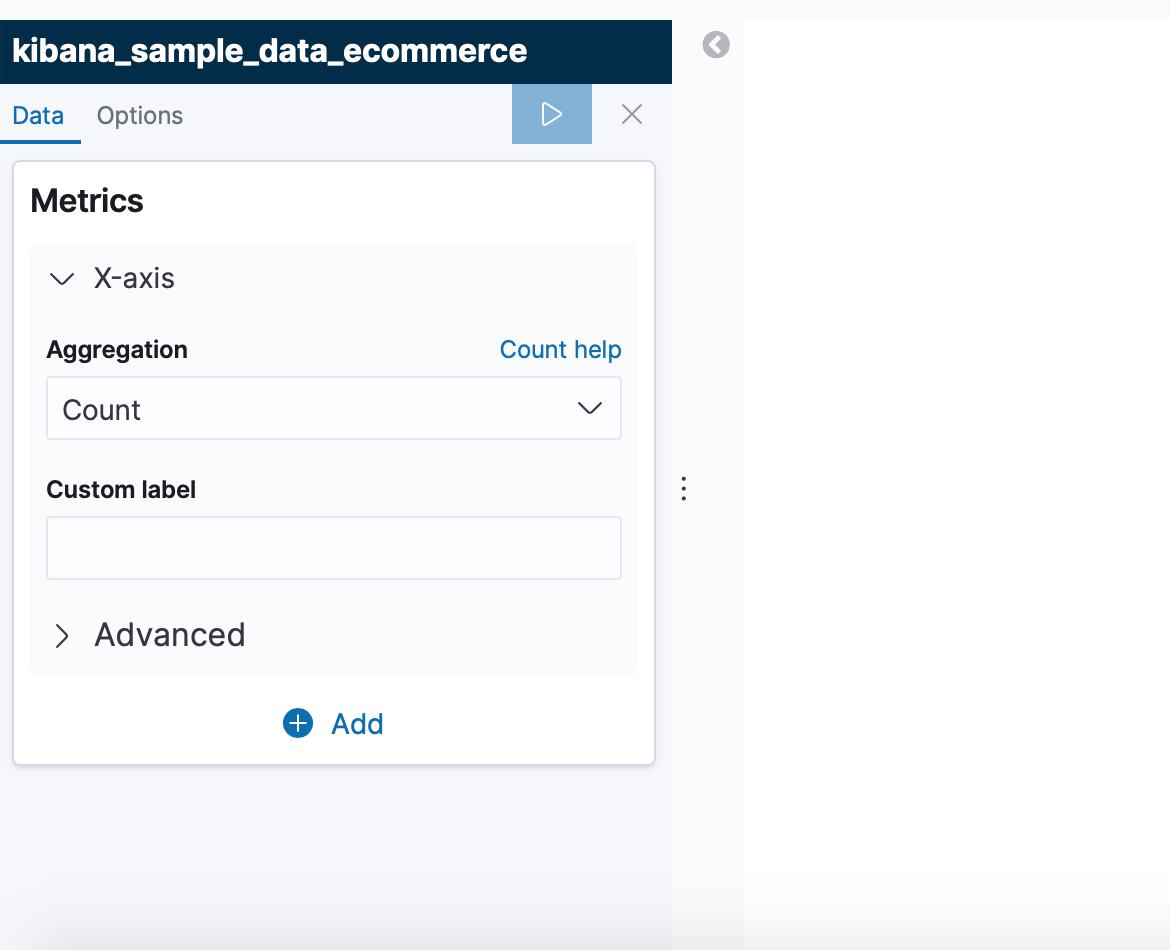
\includegraphics[width=10cm, keepaspectratio]{img/development/editor-resultado.png}
  \caption{Resultado del Editor}
  \label{fig:editor}
\end{figure}

\subsection{Plugin Simple con datos}
Ahora que ya podemos elegir los datos en el editor de Kibana, el siguiente paso es conseguir que la visualización muestre dichos datos de forma sencilla.

Para esto debemos haber aprendido, como se vió en el sprint anterior, el funcionamiento de creación y renderizado para entender dónde Kibana recibe los datos de elasticsearch. Así que lo primero que tenemos que hacer es encontrar dónde recibimos los datos que pedimos con el editor.

Si revisamos el esquema del proceso de creación de una visualización (ver capitulo), podemos suponer que los datos que recibimos vendrán en la variable visData. Lo comprobaremos de la siguiente forma:

\begin{lstlisting}[frame=single]
  render(visData, status) {
      if (visData) {
        console.log(visData);
      }
\end{lstlisting}

Con esto podremos ver que datos recibimos en la consola del navegador.

\begin{figure}[H]
  \centering
  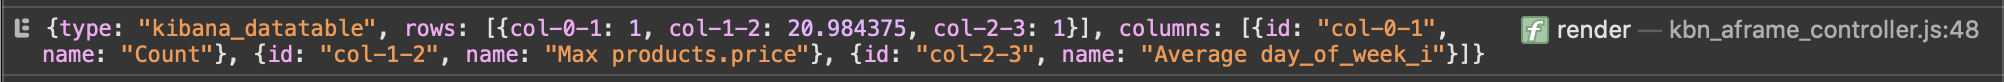
\includegraphics[width=16cm, keepaspectratio]{img/development/captura-visData.png}
  \caption{Captura de visData en la consola}
  \label{fig:visData}
\end{figure}
Esto nos sirve para analizar en cómo es el formato de los datos recibidos de elasticsearch, para luego extraer los datos que nos interesa mostrar. 

En primer lugar, vemos que se divide en 3 registros: 
\begin{itemize}
    \item \underline{type:} tipo del archivo. En este caso, kibana\_datatable.
    \item \underline{rows:} contiene únicamente los datos obtenidos en formato registro en la que la clave con la forma col-X-X que indica la posición; y el valor con el dato obtenido.
    \item \underline{columns:} contiene las etiquetas que hacen referencia a los datos obtenidos. Vienen en forma de array de registros, donde el id indica la posición del dato; y el name indica el nombre del valor. 
\end{itemize}
Analizando todo esto sacaremos los datos, con sus nombres, para guardarlo en la variable metrics.

\begin{lstlisting}[frame=single]
     const table = visData;
     const metrics = [];

      //get metrics
      table.columns.forEach((column, i) => {
        var value;
        const name = column.name;
        const id = column.id;
        table.rows.forEach(row => {
          if (row[id]){
            value = Math.round(row[id]*100)/100;
          }
        });

       metrics.push({
          name: name,
          value: value
        });
      });
\end{lstlisting}
Tras esto, lo añadimos a la visualización, de forma simple, de la siguiente forma:
\begin{lstlisting}[frame=single]
      //render metric in vis
      metrics.forEach((metric, i) => {
        const metricDiv = document.createElement('div');
        metricDiv.className = 'myvis-metric-div';
        metricDiv.innerHTML = `<b>${metric.name}:</b> 
        ${metric.value}`;
        metricDiv.setAttribute('style', `font-size: 
        ${this.vis.params.fontSize}pt`);
        this.container.appendChild(metricDiv);
      });
\end{lstlisting}
Como resultado obtenemos las figuras, que agregamos anteriormente en el capítulo anterior, seguido de los 3 valores que pedimos desde el editor.
\begin{figure}[H]
  \centering
  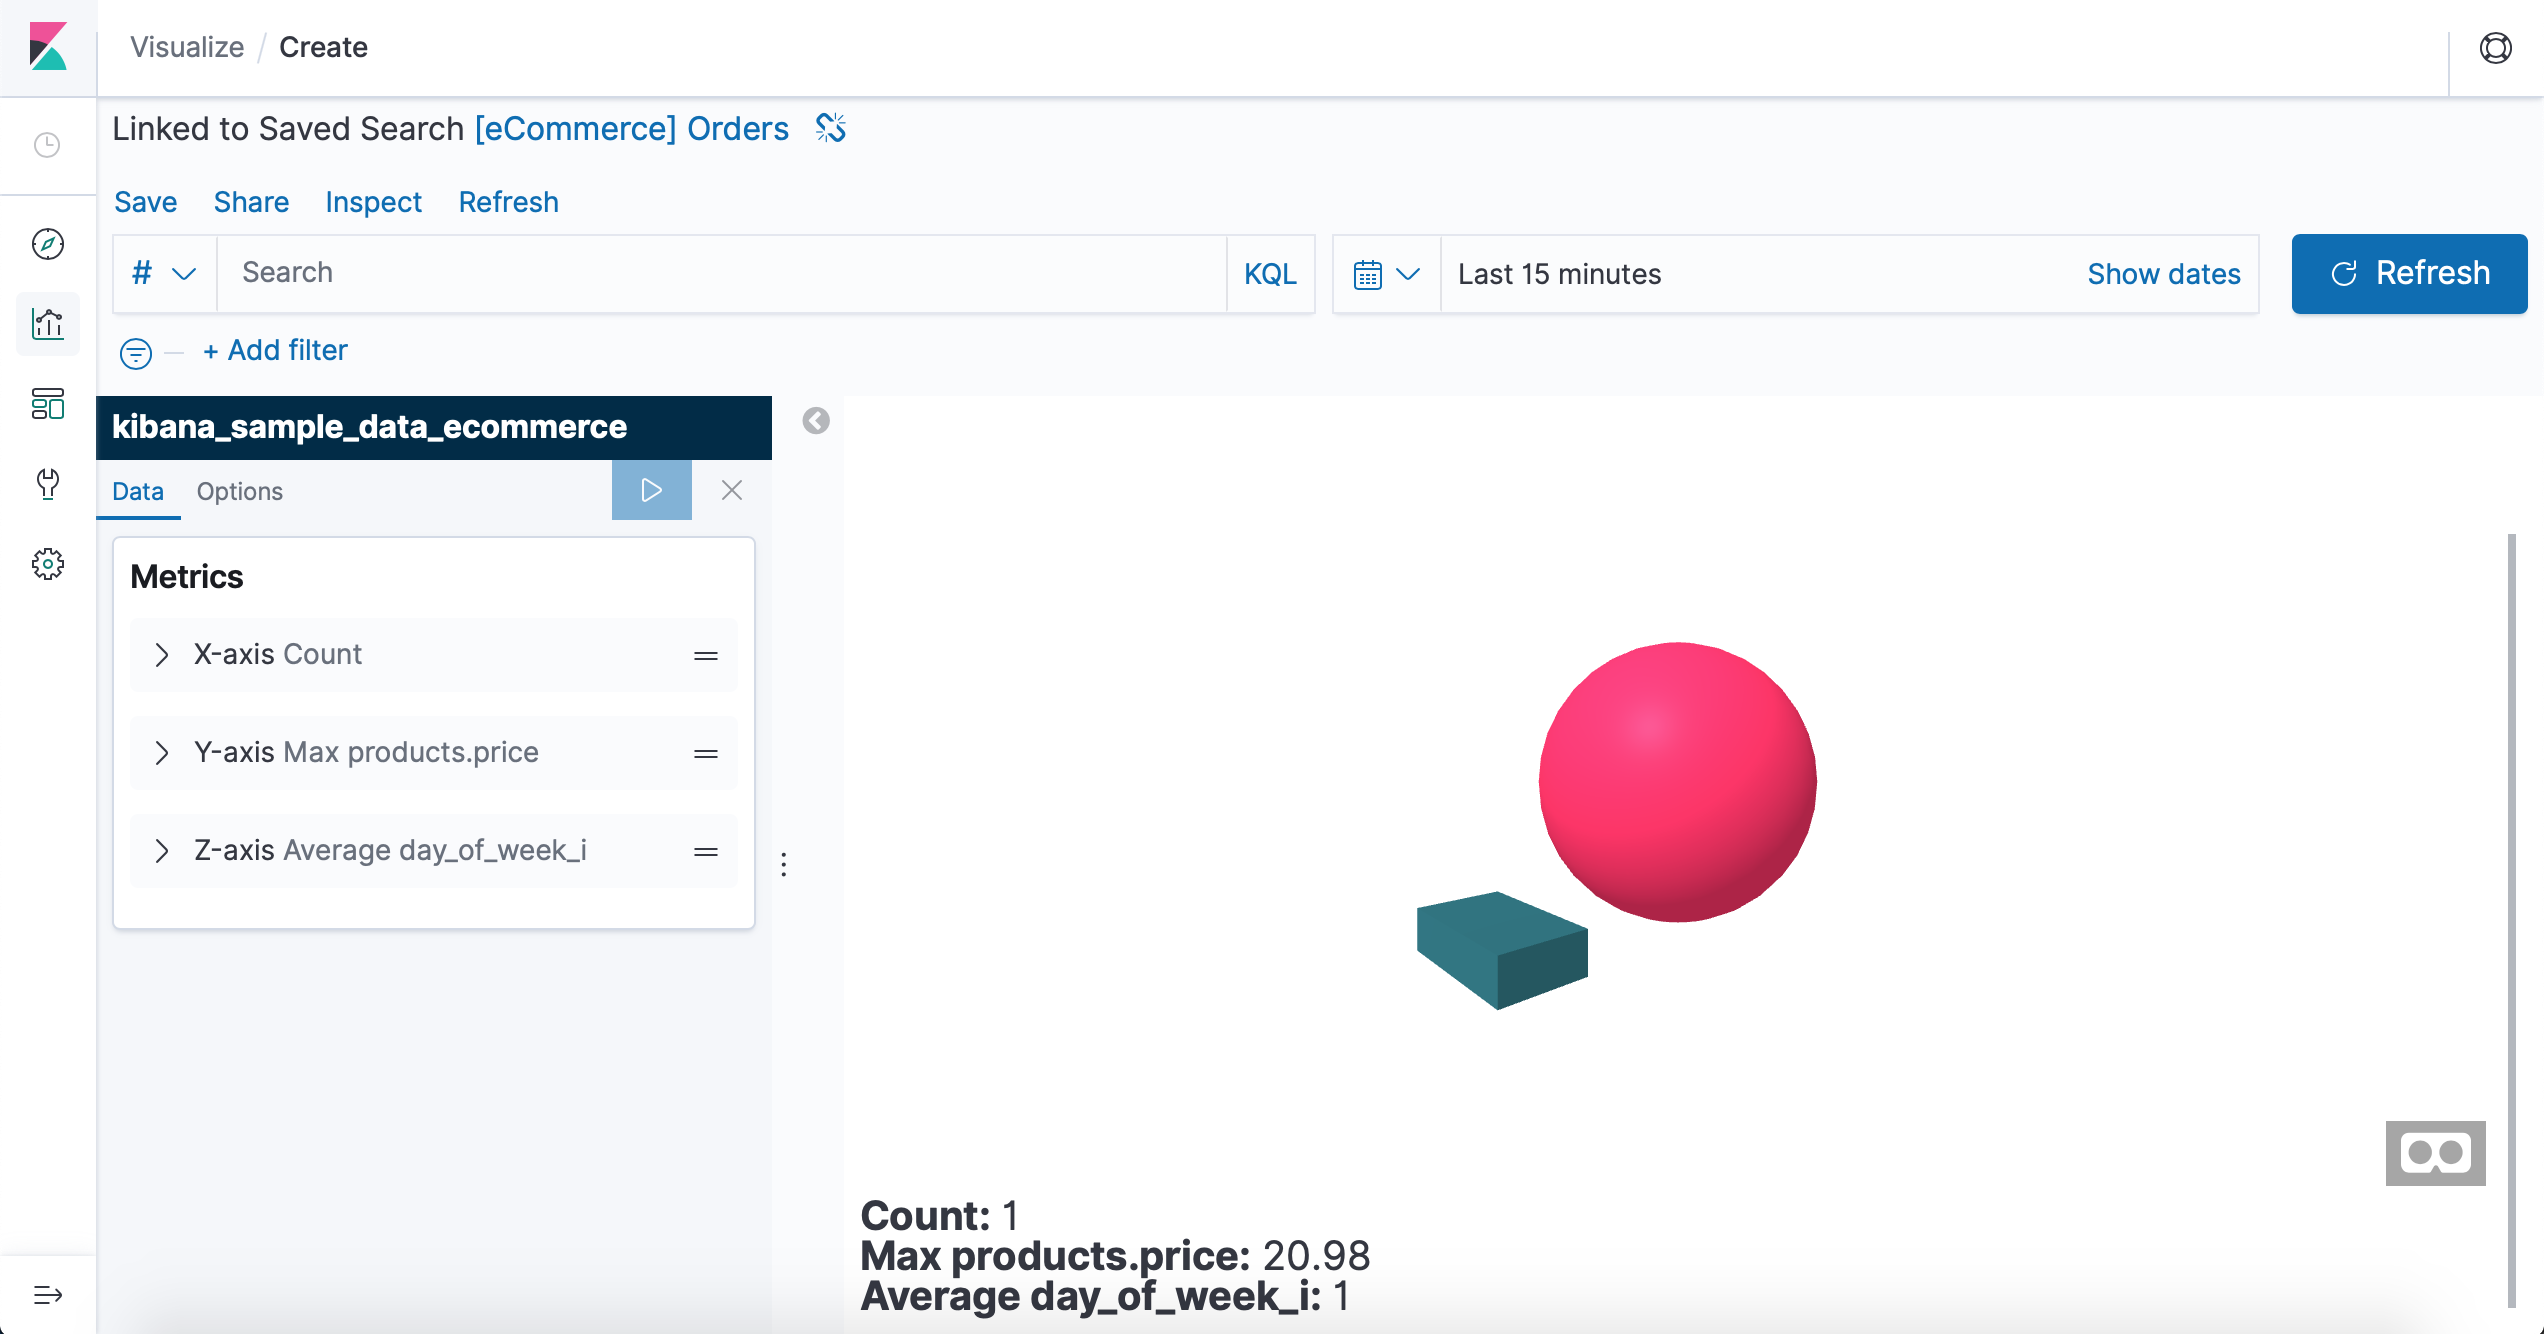
\includegraphics[width=16cm, keepaspectratio]{img/development/resultado-simple-data.png}
  \caption{Resultado Visualización con datos}
  \label{fig:simplewithdata}
\end{figure}


\subsection{Integración de A-frame con datos}
Ahora que ya hemos aprendido a obtener los datos que pedimos a elasticsearch para incluirlos en nuestra visualización, el siguiente paso es saber añadir estos datos para poder crear las figuras en base a estos datos.

Únicamente nos centraremos en crear el cubo tomando como valores las 3 métricas que pedimos desde el editor. Para ello, tenemos dos opciones:
\begin{enumerate}
    \item Insertar los datos al html usando angularJS.
    \item Crear la figura directamente desde el controller usando a-frame con javascript.
\end{enumerate}
Analizando un poco como kibana crea sus visualizaciones predeterminadas, creo que la mejor opción es la segunda y así nos ahorramos tener que usar más bibliotecas.

Por eso, eliminaremos el archivo “index.html”, eliminamos la línea donde importamos dicho archivo y cambiamos la siguiente línea de render():

\begin{lstlisting}[frame=single]
    this.container.innerHTML = '';
\end{lstlisting}

Ahora crearemos el escenario justo de donde añadimos las métricas obtenidas de elasticsearch.

\begin{lstlisting}[frame=single]
     //Creando escenario
      var escena = document.createElement('a-scene');
      escena.setAttribute('embedded', true);
\end{lstlisting}

El siguiente paso será añadir las figuras. Empezaremos por dibujar una esfera usando las primitivas que tiene a-frame. Usaremos los mismos valores que teníamos en “index.html” pero variando algún dato al gusto. Por el momento solo le añadimos los datos de forma manual porque lo único que queremos es probar cómo podemos crear una figura de esta forma.

Lo creamos de la siguiente forma:

\begin{lstlisting}[frame=single]
     // entity primitive
      var entidad = document.createElement('a-entity');
      entidad.setAttribute('geometry', {
        primitive: 'sphere',
        radius: 1.25
      });
      entidad.setAttribute('position', {
        x: -2.5,
        y: 1,
        z: -5
      });
      entidad.setAttribute('material',{
        color: '#EF2D5E'
      });
      entidad.setAttribute('shadow', true);

      escena.appendChild(entidad);
\end{lstlisting}

Esta última línea, añade la figura en el escenario anteriormente creado.

Ahora que está creado todo la escena con la figura, la añadimos el contenedor de la visualización para que nos la muestre en Kibana.

\begin{lstlisting}[frame=single]
     this.container.appendChild(escena);
\end{lstlisting}

Obteniendo como resultado la siguiente visualización.

%\begin{figure}[H]
  %\centering
  %\includegraphics[width=16cm, keepaspectratio]{img/development/}
  %\caption{Esfera A-Frame con Javascript}
 % \label{fig:onlysphere}
%\end{figure}

Una vez hemos conseguido que nos dibuje la esfera, haremos el mismo procedimiento para crear el cubo pero con un par de variaciones:

\begin{enumerate}
    \item Usaremos el cubo que creamos por componente.
    \item Añadiremos los datos obtenidos de elasticsearch.
\end{enumerate}

Como usaremos el componente, revisaremos que “box.js” este importado en el controlador.

Ahora, declaramos un array con las dimensiones que vamos a usar para crear el cubo. 

\begin{lstlisting}[frame=single]
     const axis = [];
\end{lstlisting}
Y añadimos los valores en la variable axis tras añadirlo también en metrics.
\begin{lstlisting}[frame=single]
       // add axis
        axis.push(value);
\end{lstlisting}
Por último, solo nos queda crear la figura de la misma forma y añadirlo en la escena:
\begin{lstlisting}[frame=single]
     // entity con box.js
      var caja = document.createElement('a-entity');
      caja.setAttribute('box', {
        height: axis[0]/10, //0.5
        width: axis[1]/10, //0.25
        depth: axis[2]/10, //1
      });
      caja.setAttribute('position', {
        x: 0,
        y: 1,
        z: -5
      });
      caja.setAttribute('rotation', {
        x: 0,
        y: -45,
        z: 0
      });
      caja.setAttribute('material', 'color', '#4CC3D9');

      escena.appendChild(caja);
\end{lstlisting}
Como se ve, la diferencia con la esfera es que creamos un a-entity con el atributo ‘box’ y no ‘geometry’ y dándole los datos que declaramos en el constructor de box.js.

Con esto, obtenemos como resultado un cubo que varía en base a los datos que le pedimos a elasticsearch.

\begin{figure}[H]
  \centering
  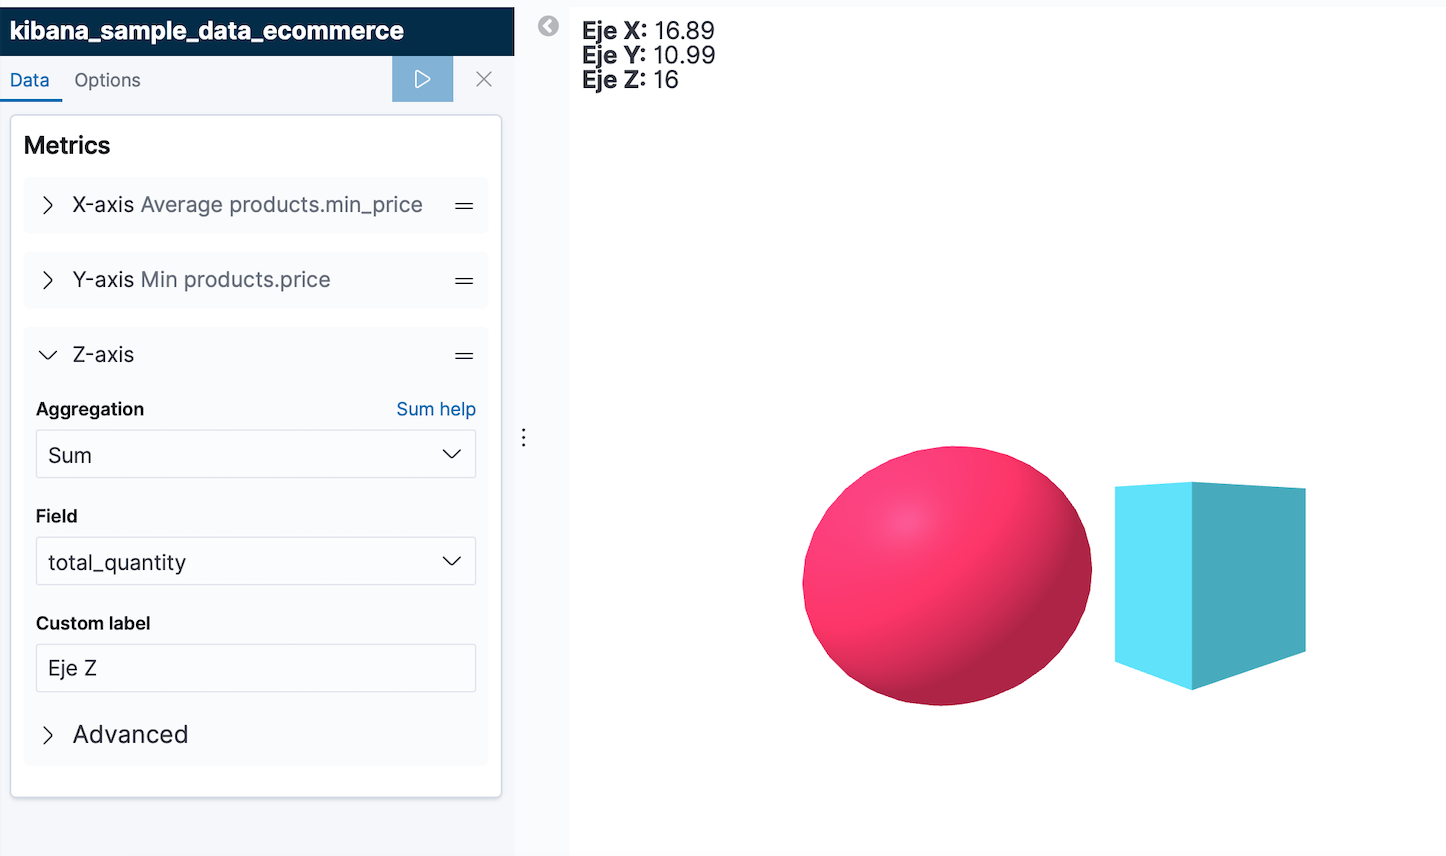
\includegraphics[width=16cm, keepaspectratio]{img/development/box_with_data.png}
  \caption{Resultado de integración de A-Frame con datos}
  \label{fig:boxwithdata}
\end{figure}


%%%%%%%%%%%
% SPRINT 3
%%%%%%%%%%%

\section{Sprint 3: Implementación de BabiaXR }
\label{sec:sprint3}

Tras haber completado toda la parte básica en cuanto a la creación de un plugin para kibana y la integración de gráficos VR usando A-frame, procederemos a integrar la biblioteca de BabiaXR. 

Como explicamos anteriormente (ver capítulo) BabiaXR es una biblioteca de componentes donde cada componente es un tipo de gráfica y por tanto será un tipo de visualización de nuestro plugin.

Para este sprint, cogereremos un solo componente de BabiaXR y lo integraremos en nuestro plugin. El componente elegido será “geopiechart” que nos creará un visualización que nos mostrará una gráfica de tipo pie. 

Al igual que hicimos en el anterior sprint, dividiremos el sprint en dos partes:

\begin{enumerate}
    \item Integraremos pie chart sin usar datos.
    \item Integraremos pie chart usando datos.
\end{enumerate}

\subsection{Visualización Pie Chart sin Datos}

Anteriormente estábamos trabajando con un plugin de prueba; pero como esta parte ya será parte del resultado final, crearemos un nuevo plugin, cogiendo como referencia nuestro plugin de prueba, y lo llamaremos “kbn\_aframe”.

Para empezar, introducimos el nombre de nuestro nuevo plugin, además de agregarle el nombre del autor y las dependencias que necesitaremos. Como lo hemos hecho anteriormente, este va dentro de “package.json”.

\begin{lstlisting}[frame=single]
{
  "name": "kbn_aframe",
  "version": "0.0.1",
  "kibana": {
    "version": "7.6.0"
  },
  "authors": [
    "Andrea Villaverde <camaratomoyo@gmail.com>"
  ],
  "dependencies": {
    "aframe": ">=1.0.0",
    "aframe-babia-components": ">=1.0.5",
    "aframe-extras": ">=6.1.0",
    "aframe-environment-component": ">=2.0.0",
  }
}
\end{lstlisting}

Dependencias que necesitamos:
\begin{itemize}
    \item \underline{aframe}: para que podamos crear componente hechas con a-frame.
    \item \underline{aframe-babia-components}: biblioteca de componentes de a-frame con las gráficas que vamos a implementar.
    \item \underline{aframe-extras}: componente de aframe que añade otros tipo de controles diferentes a los que vienen de base con a-frame.
    \item \underline{aframe-environment-component}: componente de a-frame que permite crear entornos visualmente más atractivos que el que viene de base en a-frame.
\end{itemize}

También añadiremos el directorio de nuestro nuevo fichero principal, al que llamaremos kbn\_aframe.js, dentro de “index.js”.

\begin{lstlisting}[frame=single]
export default function (kibana) {
  return new kibana.Plugin({
    uiExports: {
      visTypes: [
        'plugins/kbn_aframe/kbn_aframe'
      ]
    }
  });
}
\end{lstlisting}

Y declararemos nuestra nueva visualización para registrarla posteriormente.

\begin{lstlisting}[frame=single]
name: 'pie_chart',
title: 'VR Pie',
icon: 'visPie',
description: 'Compare parts of a whole (VR Chart).',
visualization: VisController,
editor: 'default'
\end{lstlisting}

Ahora nos vamos al controlador, que hemos llamado “kbn\_aframe\_controller.js”, y lo primero que haremos será importar las dependencias que hemos instalado anteriormente.

\begin{lstlisting}[frame=single]
import 'aframe';
import 'aframe-babia-components';
import 'aframe-environment-component';
import 'aframe-extras';
\end{lstlisting}

El siguiente paso es crear nuestra visualización dentro del render tomando como referencia el ejemplo que encontramos en la documentación de BabiaXR. Para ello, lo dividiremos en varias partes:

\begin{enumerate}
    \item Crearemos el entorno y le añadiremos las luces de la escena.
    \item Añadiremos los datos de forma manual, ya que en esta ocasión estamos trabajando sin datos.
    \item Añadiremos el componente “geopiechart” a la visualización.
    \item Añadiremos los controles y la cámara a la escena. 
\end{enumerate}

Comenzamos creando el escenario a-frame, añadiendo un tipo de entornos con aframe-environment-component; y le añadiremos las luces. Para no complicarnos mucho, le pondremos luces de tipo ambiente que iluminará la escena por completo.

\begin{lstlisting}[frame=single]
//Create a_scene
var escena = escena = document.createElement('a-scene');
escena.setAttribute('id', 'AframeScene');
escena.setAttribute('embedded', true);

// Environment
var environment = document.createElement('a-entity');
environment.setAttribute('environment', {
preset: 'contact',
skyType: 'gradient'
});
escena.appendChild(environment);

// LIGHT
var light = document.createElement('a-light');
light.setAttribute('type', 'ambient');
light.setAttribute('intensity', 1);
light.setAttribute('position', { x:10, y:20, z:30 });
escena.appendChild(light);
\end{lstlisting}

Atributos utilizados dentro del componente environment:

\begin{itemize}
    \item \underline{preset}: indicas el estilo del entorno que quieres usar. Aframe-environment-component muestra un catálogo de entornos para elegir al gusto.
    \item \underline{skyType}: indica el tipo de skybox que deseas poner. Aunque puedes elegir el entorno predeterminado, también se le puede personalizar sus elementos. Este es un ejemplo de ello, el cual te permite indicar si quieres que sea un solo color o con degradado, entre otros.
\end{itemize}

Ahora procedemos a añadir los datos que vamos a necesitar para construir el componente “geopiechart”. Estos datos irán en formato json y deben seguir la estructura que viene especificada en la documentación de babiaxr.

\begin{lstlisting}[frame=single]
[{"key":"kbn_network","size":10},
{"key":"Maria","size":5},
...
]
\end{lstlisting}

Según esto construiremos los datos de la siguiente manera:

\begin{lstlisting}[frame=single]
let data_json = [{"key":"URJC","size":5},{"key":"Andrea",
"size":18},{"key":"David","size":6},{"key":"Jesus","size":2},
{"key":"Aframe","size":22}]
\end{lstlisting}

Y procedemos a crear tal y como nos lo indica la documentación de babiaxr.

\begin{lstlisting}[frame=single]
var chart = document.createElement('a-entity');
chart.setAttribute('geopiechart', {
  legend: true,   // legend
  axis: true,       // axis
  data: data_json      // data
});
chart.setAttribute('position', { x: 0, y: 2, z: -4 });
chart.setAttribute('rotation', { x: 90, y: -20, z: 0 });
escena.appendChild(chart);
\end{lstlisting}


Los atributos utilizados:
\begin{itemize}
    \item \underline{legend}: si deseas que al pasar por encima del elemento nos muestre su valor.
    \item \underline{axis}: si deseamos que se muestre los ejes de la gráfica, aunque en este componente no se mostrarás porque no usa ejes.
    \item \underline{data}: introduces los datos que quieres mostrar en la gráfica.
\end{itemize}

Por último, añadiremos los controles (usando aframe-extras), para que también puedan usarse en un futuro con las gafas tipo oculus, entre otras; y la cámara indicando la posición en la que queremos empezar dentro de la escena.

\begin{lstlisting}[frame=single]
var controls = document.createElement('a-entity');
controls.setAttribute('movement-controls', {fly: true});

var camera = document.createElement('a-camera');
camera.setAttribute('position', { x: 0, y: 2.5, z: 1 });
controls.appendChild(camera);

var cursor = document.createElement('a-entity');
cursor.setAttribute('cursor', {rayOrigin: "mouse"});
controls.appendChild(cursor);

var laser = document.createElement('a-entity');
laser.setAttribute('laser-controls', {hand: "right"});
controls.appendChild(laser);

escena.appendChild(controls);
\end{lstlisting}

Una vez hemos añadido todo esto, pasamos a ver el resultado en kibana.

\begin{figure}[H]
  \centering
  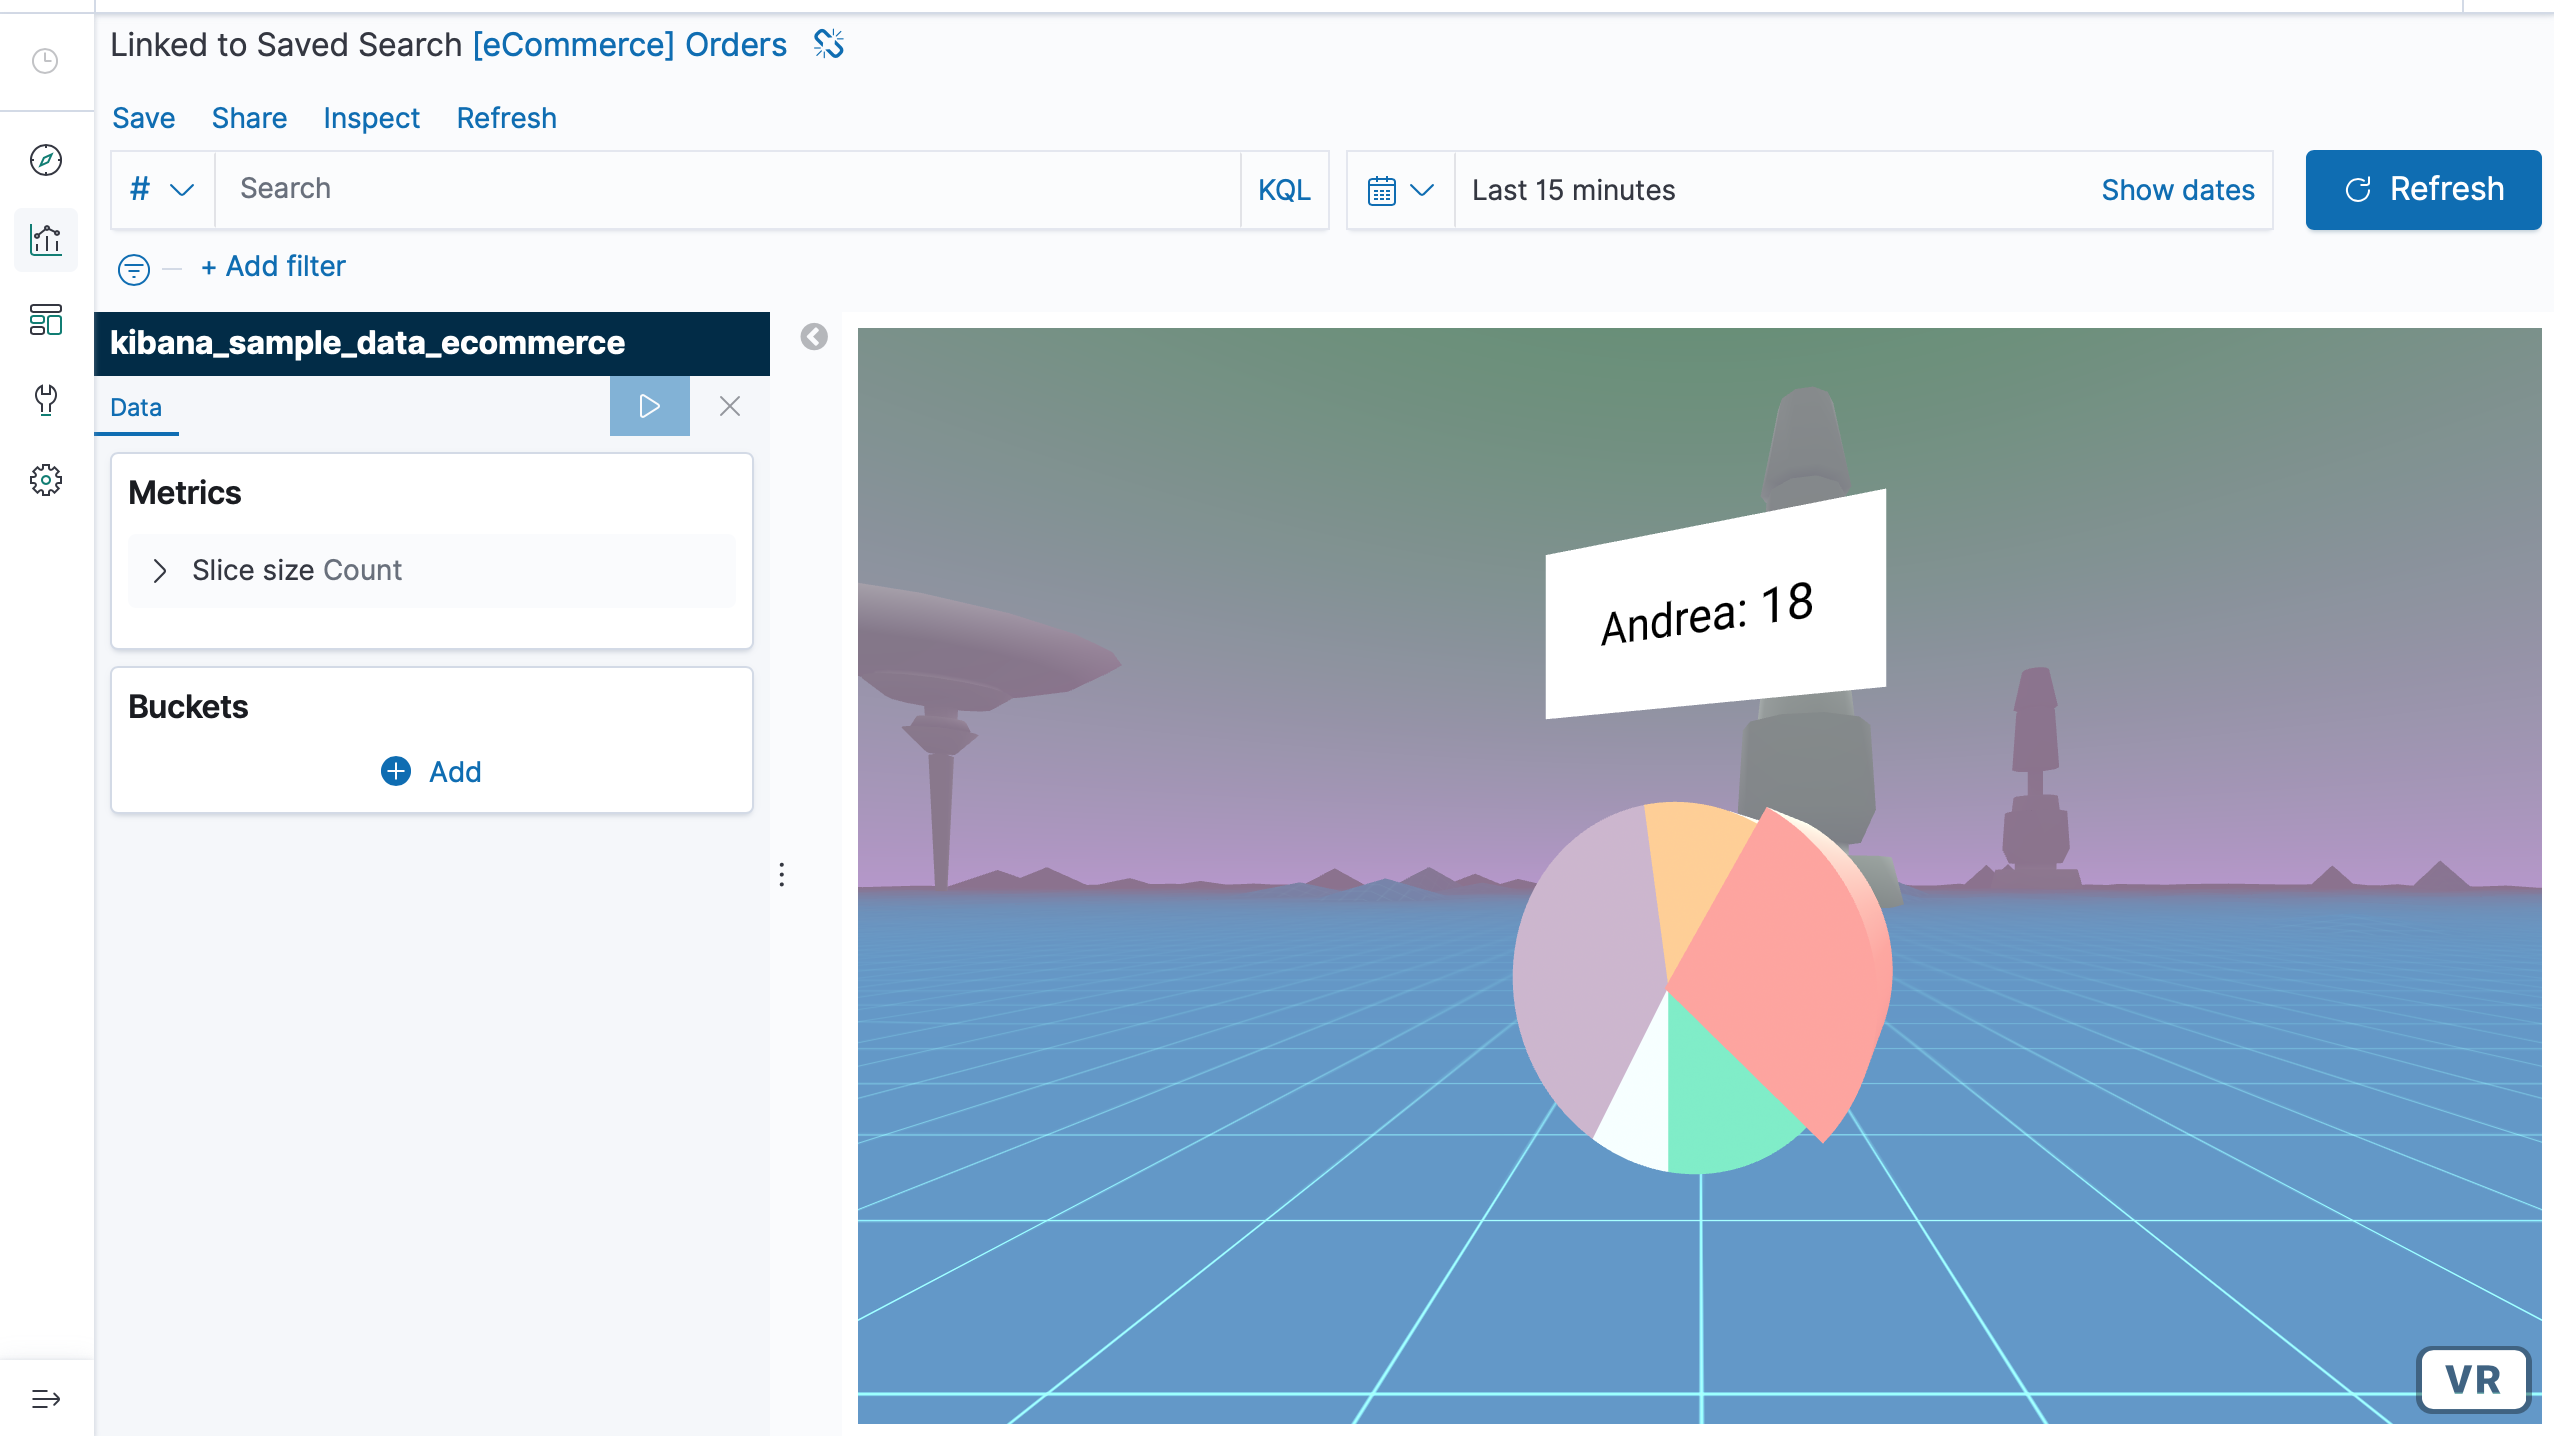
\includegraphics[width=12cm, keepaspectratio]{img/development/pie-sin-data.png}
  \caption{Resultado implementacion de geopiechart sin datos}
  \label{fig:piesindata}
\end{figure}

\subsection{Visualización Pie Chart con datos}

Ahora que ya sabemos que se puede implementar el componente de babiaxr; lo último que nos queda para terminar este sprint es hacer que se cree el componente “geopiechart” usando los datos que nos devuelve kibana de elasticsearch.

Lo primero será ver qué tipo de datos necesitaremos y lo indicaremos en el editor para que kibana pueda hacer su correspondiente.

Como trabajamos con un formato de key-size, utilizaremos un bucket que nos dará las keys y una metric que nos devolverá un valor por cada key. Una vez establecido esto, procedemos a configurar el editor, de la misma forma que lo hicimos en el sprint 2.

\begin{lstlisting}[frame=single]
editorConfig: {
  schemas: new Schemas([
    {
      group: AggGroupNames.Metrics,
      name: 'metric',
      title: 'Slice size',
      min: 1,
      max: 1,
      aggFilter: ['sum', 'count', 'cardinality', 'top_hits'],
      defaults: [{ schema: 'metric', type: 'count' }],
    },
    {
      group: AggGroupNames.Buckets,
      name: 'segment',
      title: 'Split slices',
      min: 0,
      max: 1,
      aggFilter: ['!geohash_grid', '!geotile_grid', '!filter'],
    },
  ]),
}
\end{lstlisting}

Tal y como vimos también anteriormente cuando creamos el cubo a partir de datos; tomaremos esa referencia para crear el data\_json según el formato que nos indica babiaxr.

Esta vez es la primera vez que trabajamos con un bucket, por lo que la forma de sacar las métricas será diferente, ya que ahora debemos trabajar con las keys del bucket y no solo con metrics. Es decir, en esta ocasión, meteremos en metrics los valores obtenidos en forma de diccionario.

\begin{lstlisting}[frame=single]
if ((!old_data)||(old_data != visData)){

  this.container.innerHTML = '';
  old_data = visData;
  const table = visData;
  const metrics = [];

  var id = [];
  //get metrics
  table.columns.forEach((column, i) => {
      var name = column.name;
      id.push(column.id);
   });

   table.rows.forEach(row => {
     let values = [];
     id.forEach(id => {
        if (row[id]){
           values.push(row[id]);
         };
      });
      // push metrics
      metrics.push({
         "key": values[0],
         "size": values[1]
      });
   });
}
\end{lstlisting}

Ahora nos encontramos con la situación de que el componente “geopiechart” necesita que le pasemos los datos en formato json, por lo que le damos ese formato usando la función “JSON.stringify()”.

\begin{lstlisting}[frame=single]
let data_json = JSON.stringify(metrics);
\end{lstlisting}

Con esto, hemos conseguido que a partir de ahora los datos que introducimos desde el editor sean mostrados en una gráfica tipo pie.

\begin{figure}[H]
  \centering
  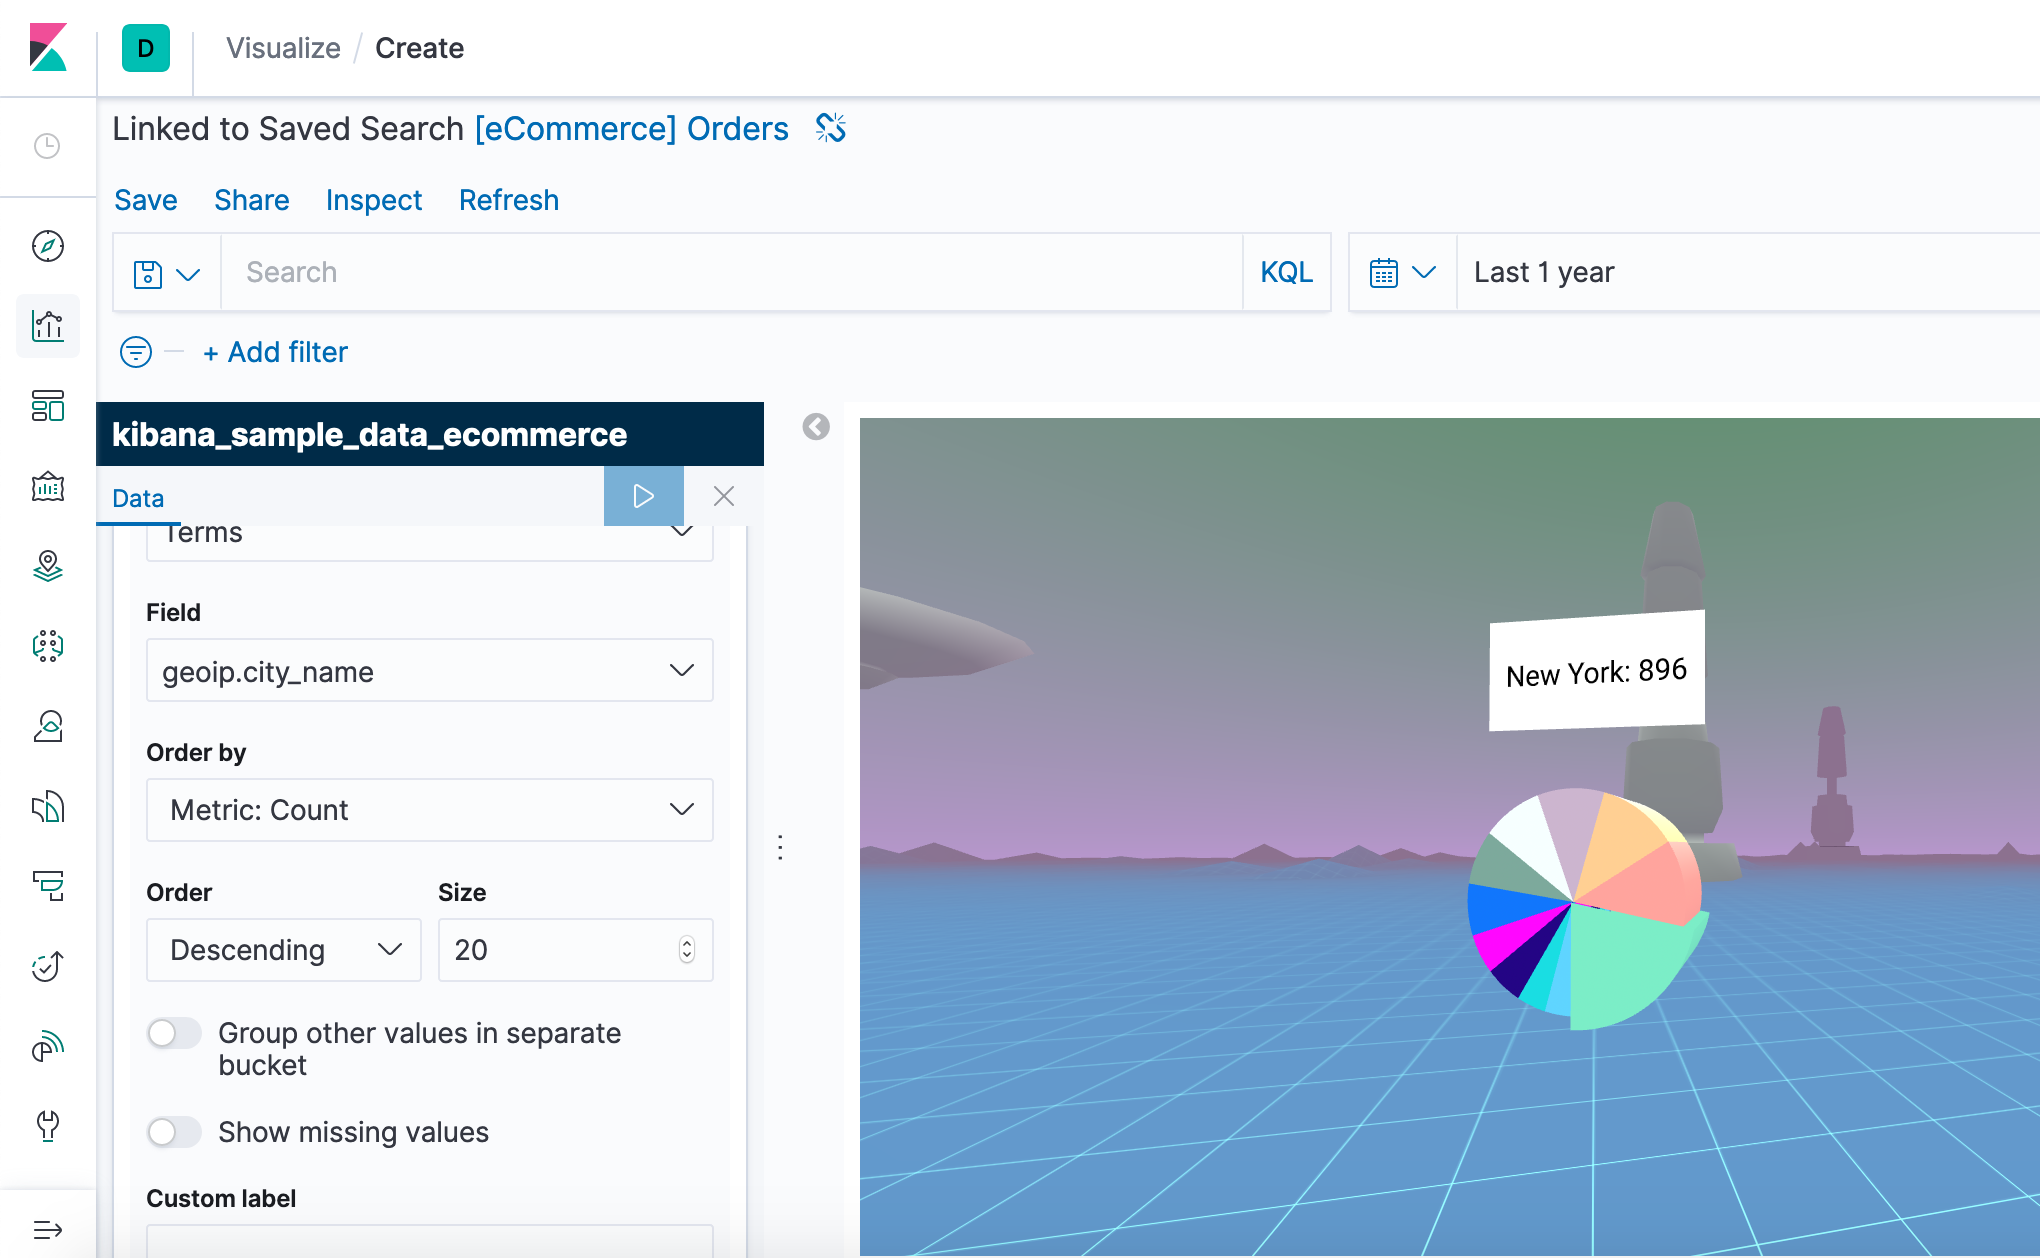
\includegraphics[width=12cm, keepaspectratio]{img/development/pie-con-data.png}
  \caption{Resultado de geopichart usando datos de Kibana}
  \label{fig:piecondata}
\end{figure}

Para obtener esta gráfica, le hemos pedido a kibana que nos muestre el número de ventas segmentadas por ciudad; y que solo nos muestre las 20 con más ventas.

%%%%%%%%%%%
% SPRINT 4
%%%%%%%%%%%

\section{Sprint 4: Nuevas Visualizaciones }
\label{sec:sprint4}

En este último sprint, incluiremos el resto de componentes que existen actualmente dentro del módulo de babiaxr. También aprovecharemos para optimizar el código y prepararlo en caso de querer añadir más características o más visualizaciones, como ocurrirá en este sprint.

Como cada componente utiliza diferentes tipos de formato a la hora de introducir los datos, iremos desde el más sencillo hasta el más complejo. Dicho esto, establecemos que las tareas de este sprint serán:

\begin{enumerate}
    \item Crear visualización con geosimplebarchart.
    \item Crear visualización con geo3dbarchart.
    \item Crear visualización con geobubblechart.
\end{enumerate}

\subsection{Visualización Simple Bar}
A primera vista parece que es muy sencillo de hacer, pero hay que tener un par de cosas en cuenta que antes no teníamos; pues esta es la primera vez que tenemos que registrar dos visualizaciones en un mismo plugin. Hasta ahora siempre habíamos trabajado con una sola visualización por plugin. 

En realidad esta parte es muy sencilla pues simplemente hay que crear otra constante con los parámetros de la visualización y registrarla. 

Analizando un poco cómo lo hacen los desarrolladores de kibana, vemos que crean las definiciones de las visualizaciones en archivos individuales que luego importan en el fichero principal y únicamente hay que registrar las visualizaciones en él. 

Por eso, comenzaremos trasladando el código con la definición de la visualización de piechart a otro fichero que llamaremos “pie.js”. 

Otro de los detalles a tener en cuenta es cómo el controlador va a saber que se trata de una gráficas u otras, ya que usaremos el mismo controlador para todas las visualizaciones que vamos a introducir. Para eso, existe un parámetros dentro de la definición de la visualización que permite pasar datos que luego recogeremos en “this.vis.params” dentro del controlador.

Este parámetros es “visConfig” y nos permite introducir datos por defecto desde la definición de la visualización o a través del editor en caso de crear una pestaña con opciones. 

Para nuestro caso, usaremos la opción por defecto y en ella le indicaremos que añada el tipo de gráfica de cada una de las visualizaciones. Esto hará que tengamos una variable que nos ayuda a identificar qué gráfica es y cómo proceder a la hora de coger las métricas y cómo construir la gráfica.

Así que, añadiremos esta líneas dentro de la definición de pie chart que ya se encuentra en “pie.js”.

\begin{lstlisting}[frame=single]
visConfig: {
  defaults: {
    type: 'pie',
  },
},
\end{lstlisting}

Al mismo tiempo, vamos a necesitar exportar la definición de la visualización de pie chart para poder importarla más adelante.

\begin{lstlisting}[frame=single]
export const pieDefinition = { 
    ...
    // definición de pie chart
};
\end{lstlisting}

Una vez que ya tenemos trasladada la definición de pie chart, crearemos otra definición para la nueva visualización. Anteriormente se mencionó que iríamos desde la más sencilla a la más compleja. Para esto analizamos el formato de cada uno de los componente que hay en kibana y los comparamos con el que ya tenemos implementado. A primera vista el componente “geosimplebarchart” es el más parecido al “geopiechart” pues su formato JSON son exactamente iguales.

Por tanto, procedemos a definir la nueva visualización en “simple\_bar.js”:

\begin{lstlisting}[frame=single]
export const simpleBarDefinition = {
    
    name: 'bar_chart',
    title: 'VR Vertical Bar',
    icon: 'visBarVertical',
    description: 'Assign a continuous variable to each axis 
                (VR Chart).',
    visualization: VisController,
    
    visConfig: {
      defaults: {
        type: 'simple_bar',
      },
    },
    
    editorConfig: {
      schemas: new Schemas([
        {
          group: AggGroupNames.Metrics,
          name: 'metric',
          title: 'Y-axis',
          min: 1,
          max: 1,
          aggFilter: ['sum', 'count', 'cardinality',
                    'top_hits'],
          defaults: [{ schema: 'metric', type: 'count' }],
        },
        {
          group: AggGroupNames.Buckets,
          name: 'segment',
          title: 'Split Chart',
          min: 0,
          max: 1,
          aggFilter: ['!geohash_grid', '!geotile_grid', 
                    '!filter'],
        },
      ]),
    }
};
\end{lstlisting}

Como se ve, hemos añadido también el “type” dentro de “visConfig” para indicarle que esta visualización es en la que queremos crear una gráfica usando el componente “geosimplebarchart”.

Lo que sigue es importar las definiciones, la que ya teníamos y la nueva, dentro de “kbn\_aframe.js”.


\begin{lstlisting}[frame=single]
import { pieDefinition } from './pie';
import { simpleBarDefinition } from './simple_bar';
\end{lstlisting}

Y registramos la nueva visualización:

\begin{lstlisting}[frame=single]
visualizations.types.createBaseVisualization
        (simpleBarDefinition);
\end{lstlisting}

Desde kibana ya se podrá ver que ya se puede crear un nuevo tipo de gráfica; pero antes haremos un par de modificaciones en la lógica de nuestro controlador; pues si lo dejamos tal cual dibujará también una gráfica tipo pie.

Para arreglar esto hemos creado el parámetro type en la definición de cada visualización. Esta se guarda dentro de la variable “this.vis.params.type” y con ella trabajamos para que cree la gráfica de forma correcta para cada caso.

\begin{lstlisting}[frame=single]
let type = this.vis.params.type
if ( type == 'pie') {
    chart.setAttribute('geopiechart', {
      legend: true,   // legend
      data: data      // data
    });
    chart.setAttribute('position', { x: 0, y: 2, z: -4 });
    chart.setAttribute('rotation', { x: 90, y: -20, z: 0 });
  } else if (type == 'simple_bar') {
    chart.setAttribute('geosimplebarchart', {
      legend: true,   // legend
      axis: true,     // axis
      data: data      // data
    });
    chart.setAttribute('position', { x: -2, y: 0, z: -5 });
    chart.setAttribute('rotation', { x: 0, y: 0, z: 0 });
}
\end{lstlisting}

Hasta esta parte, la nueva visualización funciona sin problemas; pero decidimos anteriormente que íbamos a optimizar un poco el código para que fuera un poco más fácil de comprender en caso de que alguien quiere contribuir más adelante.

Como primera parte de esta tarea pasaremos las partes que siempre será igual en todos los escenarios a otras funciones que irán en módulos a parte y que los incluiremos en el render con sus llamadas correspondientes. Estas partes serán la de creación del entorno y la de insertar la camara y controles. Lo haremos de esta manera porque una parte tiene más que ver con el aspecto estético de la escena y el otro más con la parte del manejo y controles sobre la escena.

Empezamos trasladando el código en el que creamos la escena, el entorno y las luces a un función “CreateScene()” que exportamos. Este fichero los nombramos “a\_scene.js”.

\begin{lstlisting}[frame=single]
function createScene (){
  //Create a_scene
  var escena = escena = document.createElement('a-scene');
  ...
  //añadimos environment y lights
  return escena;
}

export { createScene };
\end{lstlisting}

Hacemos lo mismo con la líneas correspondientes a la creación de los controles y la cámara; y lo metemos en la función “createControls()” dentro del nuevo fichero “a\_controls.js”.

\begin{lstlisting}[frame=single]
function createControls (){
 ...
  //añadimos controls y camera
  return controls;
}

export { createControls };
\end{lstlisting}

Hecho esto, importamos estas funciones en “kbn\_controller.js” y hacemos las llamadas correspondiente donde antes teníamos esa parte de código.

\begin{lstlisting}[frame=single]
import { createScene } from './a_scene';
import { createControls } from './a_controls';
...
          let escena = createScene();
          let controls = createControls();

          escena.appendChild(controls);
          escena.appendChild(chart);
          this.container.appendChild(escena);
\end{lstlisting}

Finalmente podemos irnos a Kibana para ver los resultados.

\begin{figure}[H]
  \centering
  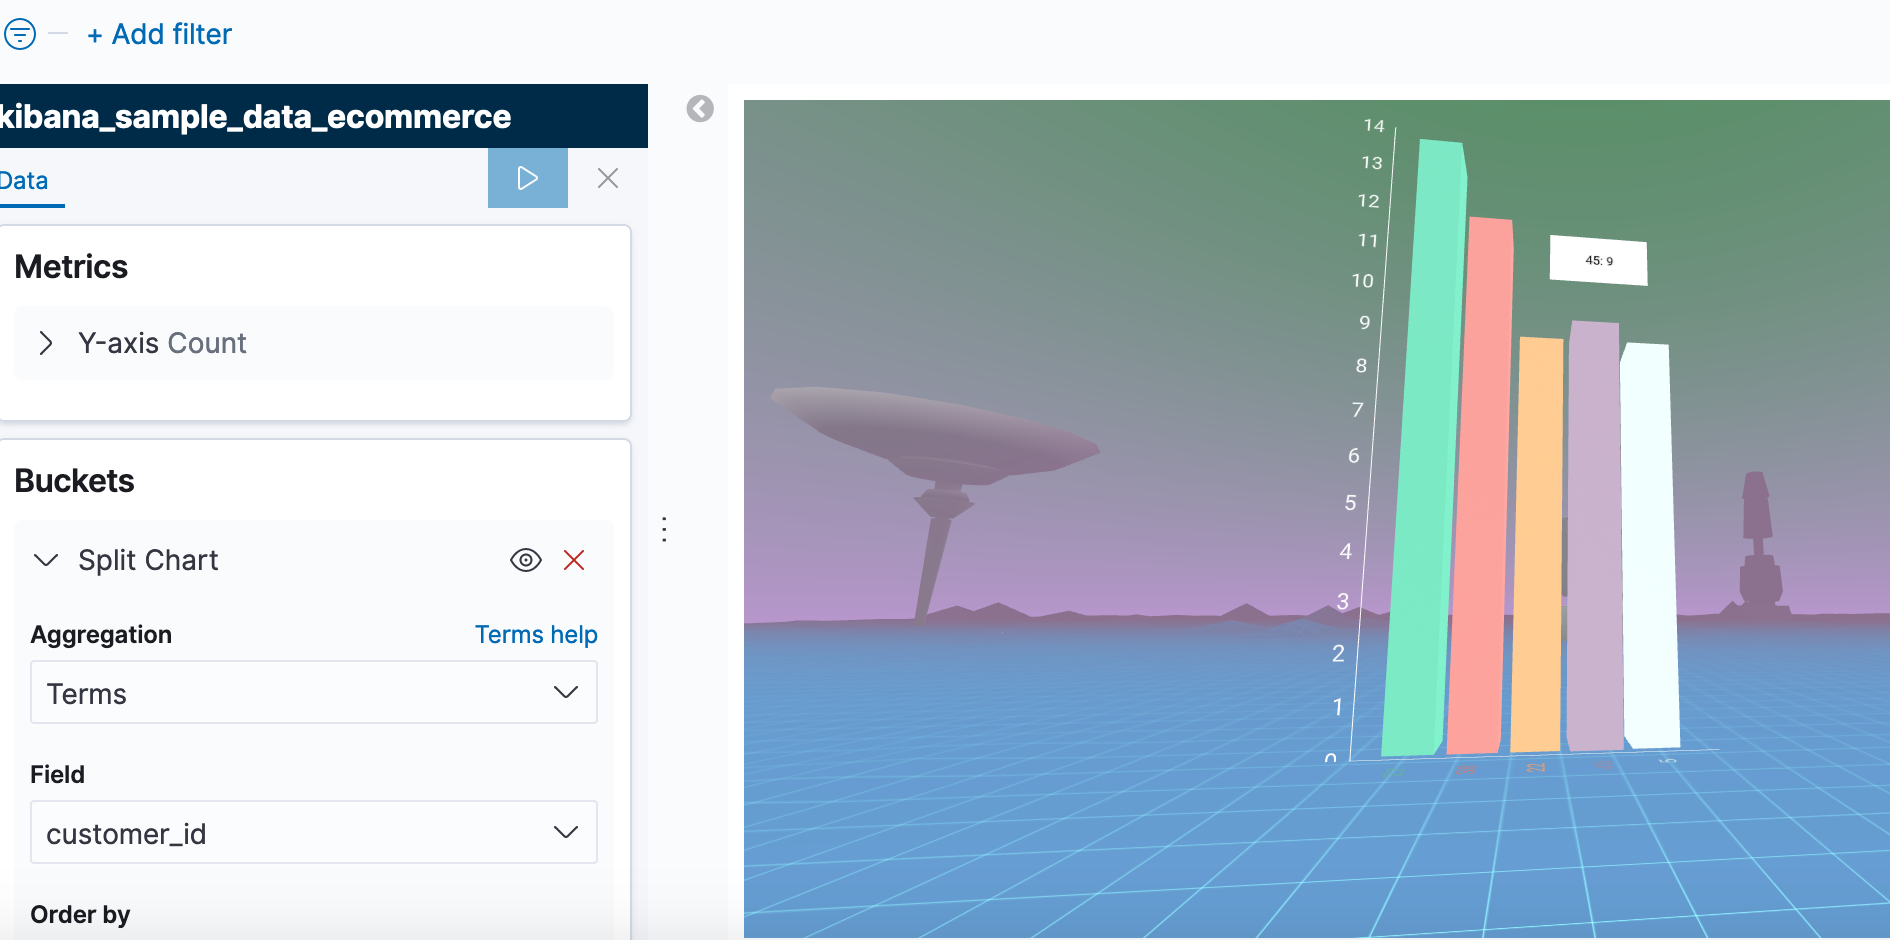
\includegraphics[width=12cm, keepaspectratio]{img/development/barchart.png}
  \caption{Resultado visualización Simple Bar Chart}
  \label{fig:simplebarchart}
\end{figure}

Para este ejemplo le hemos pedido que nos muestre lo usuarios que han hecho más compras durante un periodo de tiempo, se les etiqueta por id de usuario; y que nos muestre con la altura de la barra la cantidad de dichas compras.

\subsection{Visualización 3D Bars}

Seguimos incluyendo nuevas visualizaciones. En esta ocasión agregaremos una visualización que creará un gráfica de barras en 3D usando el componente “geo3dbarchart”. A partir de aquí, los componentes que añadamos no tendrán el mismo formato JSON como tenian “geopiechart” y “geosimplebarchart”.

\begin{lstlisting}[frame=single]
[{"key":"David","key2":"2019","size":9},
{"key":"David","key2":"2018","size":8},
...
]
\end{lstlisting}

Analizando el formato JSON de “geo3dbarchart”, vemos que en esta ocasión existe una nueva variable que es “key2”. Esta indica que, al igual que “key”, corresponde a una forma de etiquetar cada valor mostrado, en este caso serán dos etiquetas por valor. Esto. en términos visuales, lo que hará es etiquetar las barras en los ejes X y Z. 

Una vez hemos comprendido esto, ya podemos determinar como será nuestro editor. Trabajaremos con 2 claves y un valor, lo que en término del editor de kibana se traduce en 2 buckets y un metric. 

Determinado esto, procedemos a crear la definición de la nueva visualización en “3dbar.js”.

\begin{lstlisting}[frame=single]
export const geo3dBarDefinition = {

    name: '3dbar_chart',
    title: 'VR Vertical Bar 3D',
    icon: 'visBarVertical',
    description: 'Assign a continuous variable to each axis 
                (VR Chart).',
    visualization: VisController,

    visConfig: {
      defaults: {
        type: '3d_bar',
      },
    },

    editorConfig: {
      schemas: new Schemas([
        {
          group: AggGroupNames.Metrics,
          name: 'metric',
          title: 'Y-axis',
          min: 1,
          max: 1,
          aggFilter: ['sum', 'count', 'cardinality',
                    'top_hits'],
          defaults: [{ schema: 'metric', type: 'count' }],
        },
        {
          group: AggGroupNames.Buckets,
          name: 'segment',
          title: 'Split Chart',
          min: 2,
          max: 2,
          aggFilter: ['!geohash_grid', '!geotile_grid', 
                    '!filter'],
        },
      ]),
    }
 };
\end{lstlisting}

Como se ve en la configuración del editor, le estamos indicando que debe tener 2 buckets porque sino la gráfica no se dibujará.

Y procedemos a registrarla dentro en “kbn\_aframe”.

\begin{lstlisting}[frame=single]
import { geo3dBarDefinition } from './3d_bar';
...
visualizations.types.createBaseVisualization
    (geo3dBarDefinition);
\end{lstlisting}

Ahora que hemos registrado la visualización, pasamos a la parte del controlador. Empezando por la parte de la obtención de los datos que luego pasamos a JSON para luego crear su correspondiente gráfica. A cada caso que metemos, el código se vuelve más grande, por lo que se tomó la decisión de sacar de “render()” y crear una función “getMetrics()” para solo centrarnos en esa parte. 

Esta función se encontrará en un fichero “metrics.js”, donde le introduciremos los datos y el tipo de visualización para que nos devuelva sus correspondientes datos, perfectamente estructurados según el formato de cada tipo, para posteriormente convertirlos en JSON.

\begin{lstlisting}[frame=single]
function getMetrics (table, type){
  var metrics = [];
  var id = [];

  if (table.columns.length == 1){
    //only one
    var name = table.columns[0].name;
    var size = table.rows[0][table.columns[0].id];
    metrics.push({
      "key": name,
      "size": size
    });
  } else {
    table.columns.forEach((column, i) => {
      var name = column.name;
      id.push(column.id);
    });

    table.rows.forEach(row => {
      let values = [];
      id.forEach(id => {
        if (row[id]){
          values.push(row[id]);
        };
      });
      // push metrics
      if ( type == '3d_bar'){
        metrics.push({
          "key": values[0].toString(),
          "key2": values[1].toString(),
          "size": values[2],
        });
      } else if ((type == 'simple_bar')||(type == 'pie')) {
        metrics.push({
          "key": values[0].toString(),
          "size": values[1],
        });
      } ;
    });
  }
  return metrics;
}

export { getMetrics };
\end{lstlisting}

Una vez hemos trasladado el código con sus correspondientes modificaciones para el caso de la nueva visualización, procedemos a importar la función y llamarla donde antes teníamos las líneas para obtener las métricas.

\begin{lstlisting}[frame=single]
import { getMetrics } from './metrics';
...
let metrics = getMetrics(table, this.vis.params.type);
\end{lstlisting}

Por último nos faltaría añadir el caso del nuevo componente en la parte donde creamos las gráficas; pero ,al igual que con la obtención de métricas, nos encontramos que a cada caso nuevo que añadimos, el código se vuelve más complejo. Por lo que los sacaremos también y lo metemos en una nueva función “createChart()” dentro de un nuevo fichero “a\_charts.js”.

A esta función se le pasar los datos, ya en JSON, y el tipo de visualización en la que estamos; y nos devolverá la entidad que contiene la gráfica correspondiente para luego añadirla a la escena.

A esto, le añadimos también las nuevas líneas con el caso para crear una gráfica con el componente “geo3dbarchart”.

\begin{lstlisting}[frame=single]
function createChart (type, data) {
  var chart = document.createElement('a-entity');

  if ( type == 'pie') {
    chart.setAttribute('geopiechart', {
      legend: true,   // legend
      data: data      // data
    });
    chart.setAttribute('position', { x: 0, y: 2, z: -4 });
    chart.setAttribute('rotation', { x: 90, y: -20, z: 0 });
  } else if (type == 'simple_bar') {
    chart.setAttribute('geosimplebarchart', {
      legend: true,   // legend
      axis: true,     // axis
      data: data      // data
    });
    chart.setAttribute('position', { x: -2, y: 0, z: -5 });
    chart.setAttribute('rotation', { x: 0, y: 0, z: 0 });
  } else if (type == '3d_bar') {
    chart.setAttribute('geo3dbarchart', {
      legend: true,   // legend
      data: data      // data
    });
    chart.setAttribute('position', { x: 0, y: 0, z: -15 });
    chart.setAttribute('rotation', { x: 0, y: 0, z: 0 });
  };
  return chart;
}

export { createChart };
\end{lstlisting}

Y por último, importamos al función al controlador y hacemos la llamada donde corresponde.

\begin{lstlisting}[frame=single]
import { createChart } from './a_charts';
...
let chart = createChart(this.vis.params.type, data_json);
\end{lstlisting}

Con esto obtenemos la siguiente visualización en Kibana.

\begin{figure}[H]
  \centering
  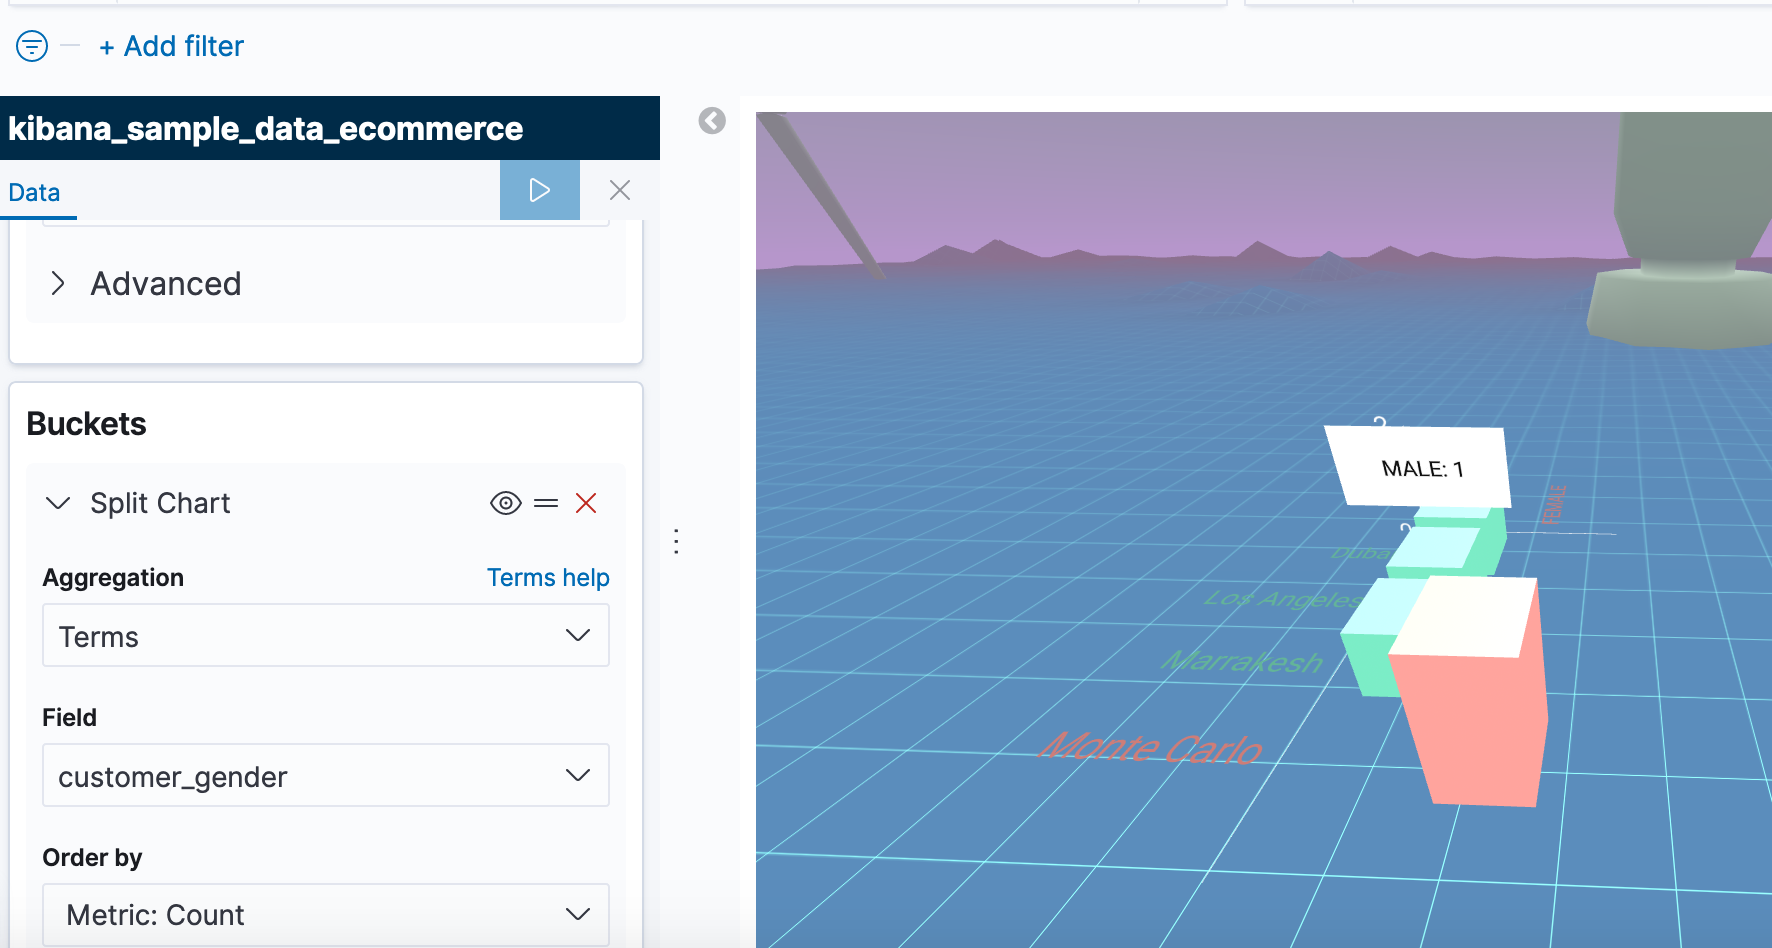
\includegraphics[width=12cm, keepaspectratio]{img/development/3d-bar-chart.png}
  \caption{Resultado Visualización 3D Bars Chart.}
  \label{fig:3dbarchart}
\end{figure}

Para este ejemplo, le hemos pedido que nos muestre las ventas que se han realizado en función del género de comprador y la ciudad donde se ha realizado la compra.

\subsection{Visualización Bubbles}

Por último, sólo nos queda crear la visualización de tipo bubbles. A partir de aquí será más sencillo pues al haber reestructurado el código, según van apareciendo nuevos casos, únicamente habrá que añadir las líneas correspondientes a dicho caso.

Al igual que hemos hecho anteriormente con el resto de visualizaciones, empezaremos determinando cómo vamos a tratar los datos.

Según la documentación de BabiaXR para el componente “geobubblechart”, el formato de nuestro JSON deberá ser el siguiente:

\begin{lstlisting}[frame=single]
[{"key":"David","key2":"2019","height":1,"radius":9},
{"key":"David","key2":"2018","height":2,"radius":8},
...
]
\end{lstlisting}

Como vemos, en esta ocasión vamos a trabajar con dos claves: “key” y “key2”; con dos valores: “height” y “radius. Esto, en términos del editor de kibana, lo traducimos en dos buckets y dos metrics. Una vez determinado esto, procedemos a crear la definición de esta nueva visualización en “bubble.js”.

\begin{lstlisting}[frame=single]
export const bubbleDefinition = {

    name: 'bubble_chart',
    title: 'VR Bubble 3D',
    icon: 'heatmap',
    description: 'Bubbles with data (VR Chart).',
    visualization: VisController,

    visConfig: {
      defaults: {
        type: 'bubble',
      },
    },

    editorConfig: {
      schemas: new Schemas([
        {
          group: AggGroupNames.Metrics,
          name: 'metric',
          title: 'Y-axis',
          min: 2,
          max: 2,
          aggFilter: ['sum', 'count', 'cardinality', 
                    'top_hits'],
          defaults: [{ schema: 'metric', type: 'count' }],
        },
        {
          group: AggGroupNames.Buckets,
          name: 'segment',
          title: 'Split Chart',
          min: 2,
          max: 2,
          aggFilter: ['!geohash_grid', '!geotile_grid', 
                    '!filter'],
        },

      ]),
    }
};
\end{lstlisting}

Y, al igual que hicimos con las anteriores visualizaciones, lo importamos a “kbn\_aframe.js” y registramos la visualización.

\begin{lstlisting}[frame=single]
import { bubbleDefinition } from './bubble';
...
visualizations.types.createBaseVisualization(bubbleDefinition);
\end{lstlisting}

Nos vamos a la parte del controlador; pero en esta ocasión directamente editaremos sobre las funciones de “getMetrics()” y “createChart()” que se encuentran en “metrics.js” y “a\_charts.js” correspondientemente.

Siguiendo los pasos que seguimos con las otras visualización, añadimos las nuevas líneas correspondientes para estructurar los datos obtenidos de elasticsearch al formato que necesitamos para poder crear el componente en la función “getMetrics()”.

\begin{lstlisting}[frame=single]
} else if (type == 'bubble'){
        metrics.push({
          "key": values[0].toString(),
          "key2": values[1].toString(),
          "height": values[2],
          "radius": values[3],
        });
};
\end{lstlisting}

Y por último, añadir el caso de esta nueva visualización y que nos cree el componente “geobubblechart”.

Obteniendo en kibana una visualización resultado con una gráfica de tipo bubble.

\begin{figure}[H]
  \centering
  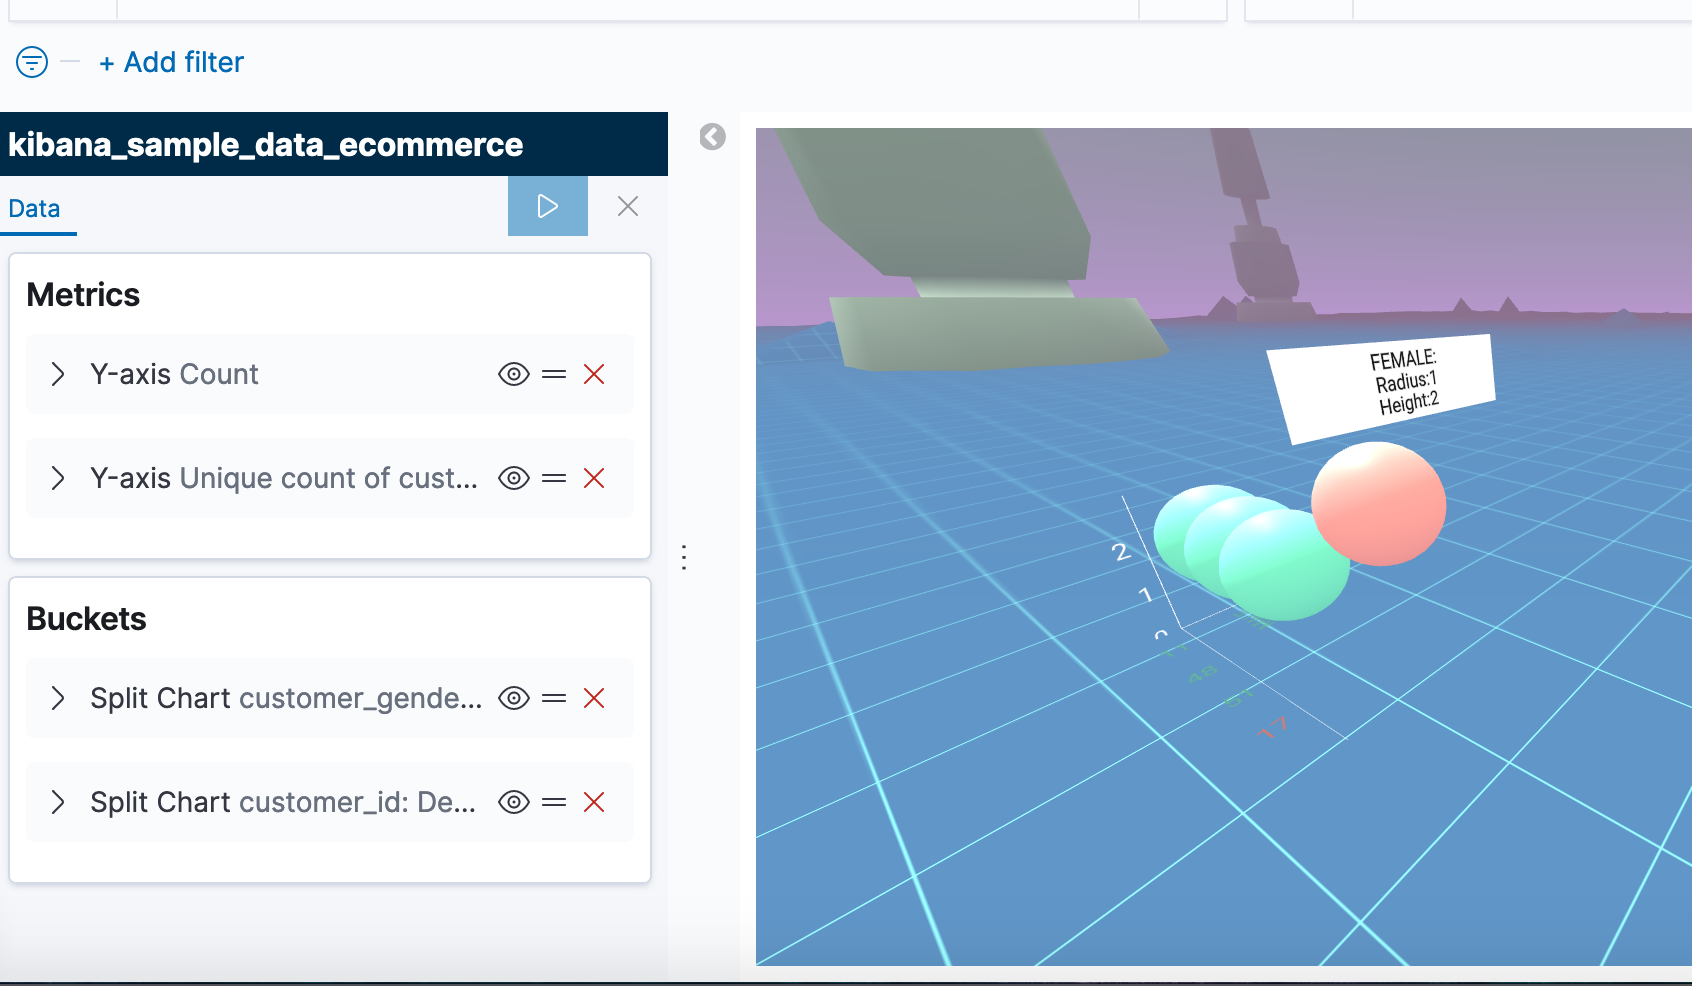
\includegraphics[width=12cm, keepaspectratio]{img/development/bubbles-chart.png}
  \caption{Resultado Visualización Bubble Chart}
  \label{fig:bubblechart}
\end{figure}

Para este ejemplo hemos tomado el número de ventas para determinar la altura, el contador uno por cada comprador y que nos los clasifique por id de usuario y según sexo.

Y tras haber añadido el último de los componente que hay actualmente en BabiaXR, damos por finalizado este sprint y con ello, finalizamos la parte de desarrollo de este proyecto.



%\begin{lstlisting}[frame=single]
%\end{lstlisting}

%\begin{figure}[H]
 % \centering
  %\includegraphics[width=16cm, keepaspectratio]{img/development/}
  %\caption{}
  %\label{fig:}
%\end{figure}


% Esto va al final de todo.
\end{document}